\documentclass[11pt, a4paper]{article}

% ── Packages ──────────────────────────────────────────────────────────
\usepackage[utf8]{inputenc}
\usepackage[T1]{fontenc}
\usepackage{lmodern}
\usepackage[margin=2.5cm]{geometry}
\usepackage{amsmath, amssymb, amsthm}
\usepackage{booktabs}
\usepackage{enumitem}
\usepackage{hyperref}
\usepackage{xcolor}
\usepackage{microtype}
\usepackage{tikz}
\usetikzlibrary{arrows.meta, positioning, decorations.pathmorphing, decorations.pathreplacing, calc, shapes.geometric, patterns, fit, backgrounds}
\usepackage{graphicx}
\graphicspath{{../experiments/results/orbit_deep/}{../experiments/results/orbit_geometry/}}
\usepackage{listings}

\hypersetup{
    colorlinks=true,
    linkcolor=black,
    citecolor=blue!60!black,
    urlcolor=blue!60!black
}

% ── Colour scheme (consistent with orn_lab_notebook.tex) ───────
\definecolor{seedred}{HTML}{E53935}
\definecolor{orbitblue}{HTML}{1E88E5}
\definecolor{targetgreen}{HTML}{43A047}
\definecolor{lookuppurple}{HTML}{7B1FA2}
\definecolor{dynamicsorange}{HTML}{FB8C00}
\definecolor{lightgray}{gray}{0.92}

% ── Code listing style ───────────────────────────────────────────────
\lstset{
    language=Python,
    basicstyle=\small\ttfamily,
    keywordstyle=\color{orbitblue}\bfseries,
    commentstyle=\color{targetgreen!70!black}\itshape,
    stringstyle=\color{seedred!80!black},
    numbers=left,
    numberstyle=\tiny\color{gray},
    numbersep=6pt,
    frame=single,
    rulecolor=\color{gray!40},
    backgroundcolor=\color{lightgray},
    breaklines=true,
    columns=fullflexible,
    showstringspaces=false,
    tabsize=4,
    aboveskip=1em,
    belowskip=1em
}

% ── Macros ────────────────────────────────────────────────────────────
\newcommand{\M}{\mathbf{M}}
\newcommand{\x}{\mathbf{x}}
\newcommand{\s}{\mathbf{s}}
\newcommand{\R}{\mathbb{R}}
\newcommand{\bigO}{\mathcal{O}}
\newcommand{\calL}{\mathcal{L}}
\newcommand{\bPhi}{\boldsymbol{\Phi}}

\newtheorem{claim}{Claim}
\newtheorem{definition}{Definition}
\newtheorem{proposition}{Proposition}
\newtheorem{theorem}{Theorem}
\theoremstyle{remark}
\newtheorem*{remark}{Remark}
\newtheorem*{intuition}{Intuition}

% ── Title ─────────────────────────────────────────────────────────────
\title{%
    \textbf{The Orbital Response Network: A Tutorial}\\[4pt]
    \Large Replacing Storage with Computation\\
    in Neural Sequence Models%
}
\author{Sirsh}
\date{March 2026 \quad{\small\textnormal{--- Tutorial Document}}}

\begin{document}
\maketitle

% ======================================================================
\begin{abstract}
A standard transformer stores its knowledge in two lookup tables: an \emph{embedding table} (one vector per token, $V \times d$ parameters) and per-layer \emph{attention projections} (separate coupling matrices at each layer, $2L \times d^2$ parameters).
This tutorial shows, from first principles, that both tables contain massive redundancy---and that both can be replaced by shared computation.

\textbf{Part 1: Computed Embeddings (Sections 2--11).}
We start with what an embedding table is (a lookup from token IDs to vectors), show why it is expensive and wasteful (at small scales, it consumes $>$90\% of model parameters), and build step by step toward the orbital alternative: a system where token representations are not stored but \emph{generated} by iterating a shared dynamical system on compressed seed vectors.
We prove this works on a clean domain (co-occurrence embeddings for TinyStories tokens: 4-dimensional seeds reconstructed to 64 dimensions at 0.90 cosine similarity), and show that orbital embeddings enable new-token interpolation that lookup tables cannot.

\textbf{Part 2: The ORN --- Orbital Attention (Section 12).}
We then tackle the deeper question: can the \emph{attention coupling rule} be shared across layers?
We build up from a concrete worked example (attention scores with actual numbers), prove the concept on a controlled task (colour matching: 16$\times$ coupling compression with no quality loss), then test on language (spectral geometry invariant at 0.98 correlation across layers in five pretrained architectures~\cite{masa2025}).
We explain why asymmetric coupling ($\M = AB^\top$) is essential for autoregressive models~\cite{altabaa2024dat}, and present scaling evidence from toy experiments through to a 108M model that beats GPT-2 Small and SmolLM-135M on 5 of 8 zero-shot benchmarks with 37--75$\times$ fewer training tokens.

\textbf{Part 3: Multimodal and V3 (Sections 15--16).}
We show that the shared coupling geometry extends across modalities~\cite{huh2024platonic}: a single $\M$ handles images, audio, and text with $>99.6\%$ coupling similarity and sub-linear rank growth.
ORN V3 extends sharing to the FFN: one wide shared feedforward network replaces 24 per-layer copies at matched parameter count, beating the per-layer baseline~\cite{onewideffn2023}.
The result is a 61M model that matches a 124M transformer---half the parameters, half of GPT-2 Small.

No prior knowledge of transformers, differential geometry, or dynamical systems is assumed.
Every concept is motivated by \emph{why} before \emph{what}, grounded with concrete numbers, and illustrated with code and diagrams.
The principle connecting all parts: \textbf{if a computation is approximately the same across instances---tokens for embeddings, layers for coupling, layers for FFN---share the parameters and iterate, rather than store separate copies.}

An emerging consensus in the 2024--2025 literature independently validates this principle: Meta-Transformer~\cite{zhang2023metatransformer} shares a frozen encoder across 12 modalities; Mixture-of-Transformers~\cite{liang2024mot} shares attention coupling while separating response; 4M-21~\cite{bachmann2024fourm} processes 21 modalities through one shared transformer.
The ORN makes this consensus \emph{explicit and measurable} through the spectral geometry of $\M$.
\end{abstract}

\tableofcontents
\newpage

% ======================================================================
\section{Two Lookup Tables, Two Kinds of Memoisation}
\label{sec:two-tables}

Before diving in, we need a map of the territory.
A standard transformer has \textbf{two separate lookup tables}, and they do fundamentally different jobs:

\begin{description}
    \item[Table 1 --- The Embedding Table \textnormal{(``what does this token mean?'')}] \hfill\\
    Maps each token ID to a vector.
    Indexed by \emph{token identity}.
    Cost: $V \times d$ parameters.
    ``Cat'' always gets the same vector, regardless of context.

    \item[Table 2 --- The Attention Projections \textnormal{(``which tokens should attend to which?'')}] \hfill\\
    At each layer $l$, separate $W_Q^{(l)}$ and $W_K^{(l)}$ matrices compute queries and keys.
    Indexed by \emph{layer number}.
    Cost: $2L \times d^2$ parameters.
    Layer 1 and layer 8 use completely different coupling rules.
\end{description}

\noindent
The broader ORN (Orbital Response Network) programme memoises \textbf{both}:

\begin{center}\small
\renewcommand{\arraystretch}{1.4}
\begin{tabular}{@{}p{3.5cm}p{4cm}p{4cm}r@{}}
\toprule
\textbf{What's replaced} & \textbf{Standard} & \textbf{Memoised} & \textbf{Savings} \\
\midrule
Per-layer coupling \newline (``Attention table'') & $2L$ separate $W_Q, W_K$ & Shared $\M = AB^\top$ \newline applied at every layer & $\bigO(Ld^2) \to \bigO(d^2)$ \\[6pt]
Per-token representations \newline (``Embedding table'') & $V \times d$ lookup & Seeds $+ \Phi$ dynamics \newline (this tutorial's topic) & $\bigO(Vd) \to \bigO(Vd_s + |\Phi|)$ \\
\bottomrule
\end{tabular}
\end{center}

\paragraph{A note on priorities.}
Table~2 (shared coupling) is the validated, practical contribution.
At 108M parameters and 8B tokens, the ORN-V2 beats GPT-2 Small (124M, 300B tokens) on 5 of 8 zero-shot benchmarks with $48\times$ fewer coupling parameters.
Spectral invariance of coupling has been confirmed across five pretrained model families~\cite{masa2025, pan2024, mu2024}.

Table~1 (orbital embeddings) is included \textbf{for pedagogical reasons}: it introduces the core principle of replacing storage with computation in the simplest possible setting, before we tackle the harder problem of attention coupling.
\textbf{In practice, orbital embeddings do not yet improve prediction quality or training efficiency} over standard embedding tables.
At production model sizes ($d \geq 512$), the embedding table is a small fraction of total parameters, and the compute overhead of iterating $\Phi$ is not justified by the compression.
Orbital embeddings may become relevant at very large vocabularies or for models that need to handle unseen tokens via seed interpolation, but for now they are a teaching tool, not a production component.

The two memoisation targets are \emph{independent and composable}: you can do either alone, or both together.
The coupling memoisation (Table~2) is what matters for the ORN architecture.

The key insight connecting them is still real: both are instances of the same principle---\textbf{if a computation is approximately the same across instances (tokens for embeddings, layers for coupling), share the parameters and iterate rather than store separate copies.}
The coupling version of this principle is proven at scale; the embedding version remains a pedagogical illustration.


% ======================================================================
\section{What Is an Embedding?}
\label{sec:embedding}

\subsection{Start from Zero: A Lookup Table}

A neural network operates on numbers, not words.
The first thing any language model must do is convert each token (word or subword) into a vector of numbers that the network can process.
An \textbf{embedding table} is the simplest way to do this: it is literally an array, indexed by token ID.

\begin{figure}[h]
\centering
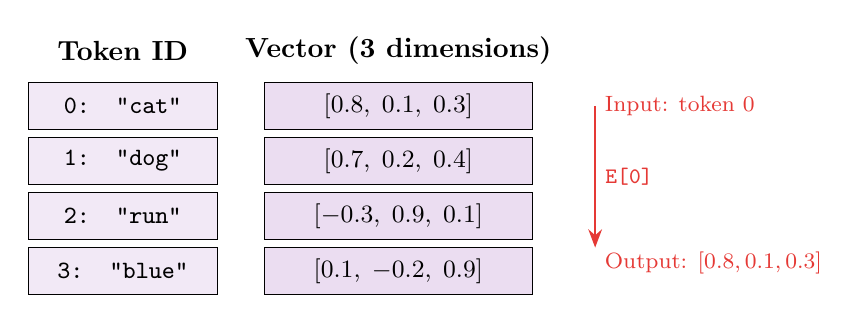
\begin{tikzpicture}[>=Stealth, font=\small]
    % Table header
    \node[font=\bfseries] at (0, 3.0) {Token ID};
    \node[font=\bfseries] at (3.5, 3.0) {Vector (3 dimensions)};

    % Row 0: cat
    \draw[fill=lookuppurple!10] (-1.2, 2.0) rectangle (1.2, 2.6);
    \node at (0, 2.3) {\texttt{0: "cat"}};
    \draw[fill=lookuppurple!15] (1.8, 2.0) rectangle (5.2, 2.6);
    \node at (3.5, 2.3) {$[0.8, \; 0.1, \; 0.3]$};

    % Row 1: dog
    \draw[fill=lookuppurple!10] (-1.2, 1.3) rectangle (1.2, 1.9);
    \node at (0, 1.6) {\texttt{1: "dog"}};
    \draw[fill=lookuppurple!15] (1.8, 1.3) rectangle (5.2, 1.9);
    \node at (3.5, 1.6) {$[0.7, \; 0.2, \; 0.4]$};

    % Row 2: run
    \draw[fill=lookuppurple!10] (-1.2, 0.6) rectangle (1.2, 1.2);
    \node at (0, 0.9) {\texttt{2: "run"}};
    \draw[fill=lookuppurple!15] (1.8, 0.6) rectangle (5.2, 1.2);
    \node at (3.5, 0.9) {$[-0.3, \; 0.9, \; 0.1]$};

    % Row 3: blue
    \draw[fill=lookuppurple!10] (-1.2, -0.1) rectangle (1.2, 0.5);
    \node at (0, 0.2) {\texttt{3: "blue"}};
    \draw[fill=lookuppurple!15] (1.8, -0.1) rectangle (5.2, 0.5);
    \node at (3.5, 0.2) {$[0.1, \; -0.2, \; 0.9]$};

    % Arrow showing lookup
    \draw[->, thick, seedred] (6.0, 2.3) -- node[right, font=\footnotesize] {\texttt{E[0]}} (6.0, 0.5);
    \node[font=\footnotesize, seedred, right] at (6.0, 2.3) {Input: token 0};
    \node[font=\footnotesize, seedred, right] at (6.0, 0.3) {Output: $[0.8, 0.1, 0.3]$};
\end{tikzpicture}
\caption{\textbf{An embedding table for four tokens.}
Each row stores a vector.
Looking up token 0 (``cat'') returns the vector $[0.8, 0.1, 0.3]$.
There is no computation---just an array read.}
\label{fig:lookup-table}
\end{figure}

\subsection{In PyTorch: It Really Is Just an Array}

\begin{lstlisting}[caption={Embedding in PyTorch: one line of code.}]
import torch.nn as nn

emb = nn.Embedding(4, 3)  # 4 tokens, 3 dimensions
# emb.weight is a 4x3 matrix of learnable parameters

token_ids = torch.tensor([0, 2])  # "cat", "run"
vectors = emb(token_ids)          # shape: (2, 3)
# This is literally: emb.weight[token_ids]
\end{lstlisting}

That is the entire mechanism.
\texttt{nn.Embedding(V, d)} creates a matrix $E \in \R^{V \times d}$ where $V$ is the vocabulary size and $d$ is the embedding dimension.
Given a token ID $w$, it returns row $w$: $\mathbf{e}_w = E[w]$.

\subsection{What Lives in the Table}

The vectors are not chosen by hand---they are \emph{learned} from data.
During training, the model adjusts the embedding vectors so that tokens appearing in similar contexts end up with similar vectors.
The result:
\begin{itemize}[nosep]
    \item ``cat'' and ``dog'' become close (both appear after ``the'', before ``ran'', etc.)
    \item ``run'' and ``jump'' become close (both are verbs of motion)
    \item ``blue'' and ``red'' become close (both are colour adjectives)
\end{itemize}
The embedding table encodes \emph{distributional similarity}: words that appear in similar contexts get similar vectors.
This structure is powerful---it is why word embeddings work at all.

\subsection{The Cost: Most of Your Parameters}

Here is the problem.
Every token gets its own independent vector.
If you have $V$ tokens and each vector has $d$ dimensions, the table has $V \times d$ parameters.
For real models:

\begin{center}\small
\begin{tabular}{@{}lrrrr@{}}
\toprule
\textbf{Model} & $V$ & $d$ & \textbf{Embedding params} & \textbf{\% of model} \\
\midrule
Our toy model & 50,257 & 36 & 1.81M & 91\% \\
GPT-2 (small) & 50,257 & 768 & 38.6M & 31\% \\
GPT-2 (medium) & 50,257 & 1024 & 51.5M & 14\% \\
LLaMA-7B & 32,000 & 4096 & 131M & 1.9\% \\
\bottomrule
\end{tabular}
\end{center}

The pattern is clear: at small model sizes, the embedding table dominates.
A 2M-parameter model with vocabulary 50K spends 91\% of its parameters just storing the lookup table, leaving almost nothing for the actual computation.
This is the \textbf{parameter dominance problem}, and it is what orbital embeddings aim to solve.


% ======================================================================
\section{How This Runs on a GPU}
\label{sec:gpu}

To understand why orbital embeddings help, you need to understand a fundamental asymmetry in modern hardware.

\subsection{The Roofline Model}

A GPU has two resources:
\begin{enumerate}[nosep]
    \item \textbf{Compute}: how many arithmetic operations per second (measured in FLOPS).
    \item \textbf{Memory bandwidth}: how many bytes per second it can load from memory.
\end{enumerate}

An NVIDIA A100 has 312 TFLOPS of compute but only 2 TB/s of memory bandwidth.
The ratio is:
\[
    \frac{312 \times 10^{12} \text{ FLOPS}}{2 \times 10^{12} \text{ bytes/s}} = 156 \text{ FLOPs per byte loaded.}
\]
This means: for every byte you load from memory, the GPU can perform 156 arithmetic operations \emph{for free} (they finish before the next byte arrives).

\begin{figure}[h]
\centering
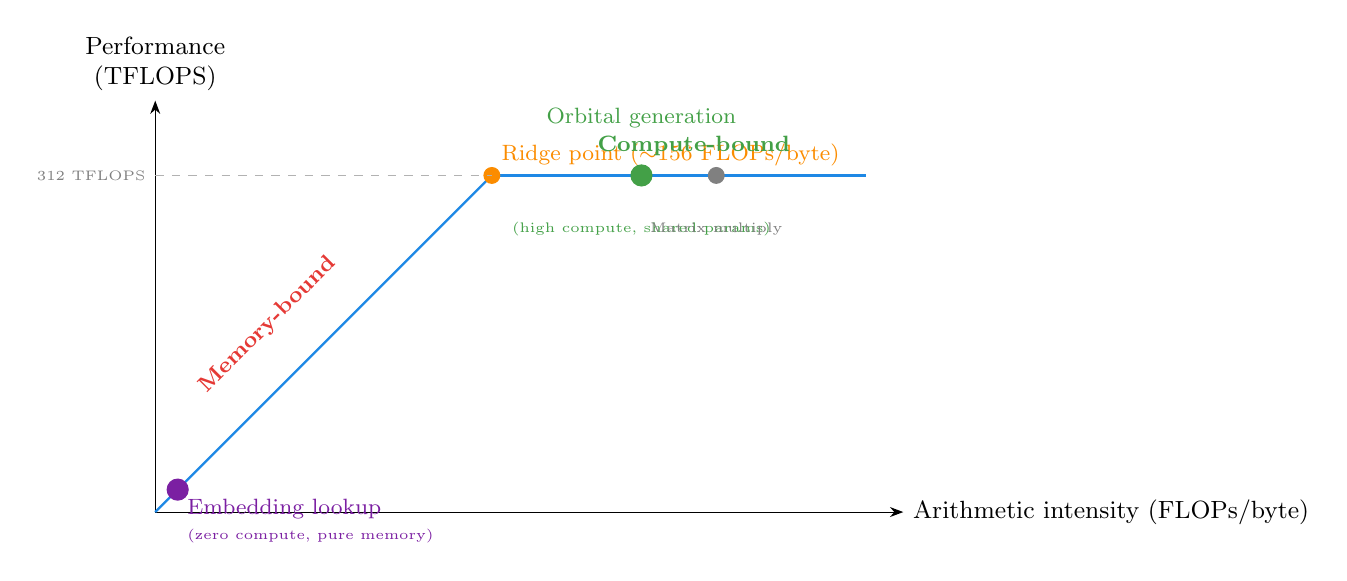
\begin{tikzpicture}[>=Stealth, font=\small, scale=0.95]
    % Axes
    \draw[->] (0, 0) -- (10, 0) node[right] {Arithmetic intensity (FLOPs/byte)};
    \draw[->] (0, 0) -- (0, 5.5) node[above, align=center] {Performance\\(TFLOPS)};

    % Roofline
    \draw[thick, orbitblue] (0, 0) -- (4.5, 4.5);  % Memory-bound slope
    \draw[thick, orbitblue] (4.5, 4.5) -- (9.5, 4.5);  % Compute-bound ceiling

    % Ridge point
    \filldraw[dynamicsorange] (4.5, 4.5) circle (3pt);
    \node[above right, dynamicsorange, font=\footnotesize] at (4.5, 4.5) {Ridge point ($\sim$156 FLOPs/byte)};

    % Labels for regions
    \node[seedred, font=\footnotesize\bfseries, rotate=45] at (1.5, 2.5) {Memory-bound};
    \node[targetgreen, font=\footnotesize\bfseries] at (7.2, 4.9) {Compute-bound};

    % Embedding lookup point
    \filldraw[lookuppurple] (0.3, 0.3) circle (4pt);
    \node[lookuppurple, font=\footnotesize, below right] at (0.3, 0.3) {Embedding lookup};
    \node[lookuppurple, font=\tiny, below right] at (0.3, -0.1) {(zero compute, pure memory)};

    % Orbital point
    \filldraw[targetgreen] (6.5, 4.5) circle (4pt);
    \node[targetgreen, font=\footnotesize, above] at (6.5, 5.0) {Orbital generation};
    \node[targetgreen, font=\tiny, below] at (6.5, 4.0) {(high compute, shared params)};

    % MatMul point for reference
    \filldraw[gray] (7.5, 4.5) circle (3pt);
    \node[gray, font=\tiny, below] at (7.5, 4.0) {Matrix multiply};

    % Peak compute line
    \draw[dashed, gray!60] (0, 4.5) -- (4.5, 4.5);
    \node[left, gray, font=\tiny] at (0, 4.5) {312 TFLOPS};
\end{tikzpicture}
\caption{\textbf{The roofline model.}
Operations below the ridge point are memory-bound: they cannot use the GPU's full compute because they spend all their time waiting for data.
Embedding lookup sits in the extreme lower-left: nearly zero arithmetic, pure memory read.
Orbital generation (matrix multiplies with shared weights) sits in the compute-bound region, where the GPU is most efficient.}
\label{fig:roofline}
\end{figure}

\subsection{Embedding Lookup: Wasting the GPU}

An embedding lookup loads one $d$-dimensional vector per token and does zero arithmetic.
Its arithmetic intensity is approximately zero.
On the roofline diagram (Figure~\ref{fig:roofline}), it sits in the extreme lower-left corner---the worst possible place.
The GPU's 312 TFLOPS of compute power are completely idle.

\subsection{The Flash Attention Precedent}

This is not a new insight.
Flash Attention (Dao et al., 2022) achieved a 7.6$\times$ speedup on GPT-2 by \emph{recomputing} attention scores instead of storing them in memory.
It performs \emph{more} FLOPs but runs faster, because the bottleneck was memory, not compute.
Gradient checkpointing applies the same principle to activations: store $\bigO(\sqrt{n})$ checkpoints, recompute the rest.

The lesson: on modern hardware, \textbf{recomputation is faster than storage} whenever the operation is memory-bound.
This is exactly our proposal for embeddings.


% ======================================================================
\section{Compression: Most of the Table Is Redundant}
\label{sec:compression}

\subsection{PCA on Real Embeddings}

If each of the $V$ vectors were truly independent, you would need all $V \times d$ parameters.
But they are not independent.
Performing PCA (Principal Component Analysis) on trained embedding matrices reveals that most of the variance is captured by a small number of directions.

\begin{figure}[h]
\centering
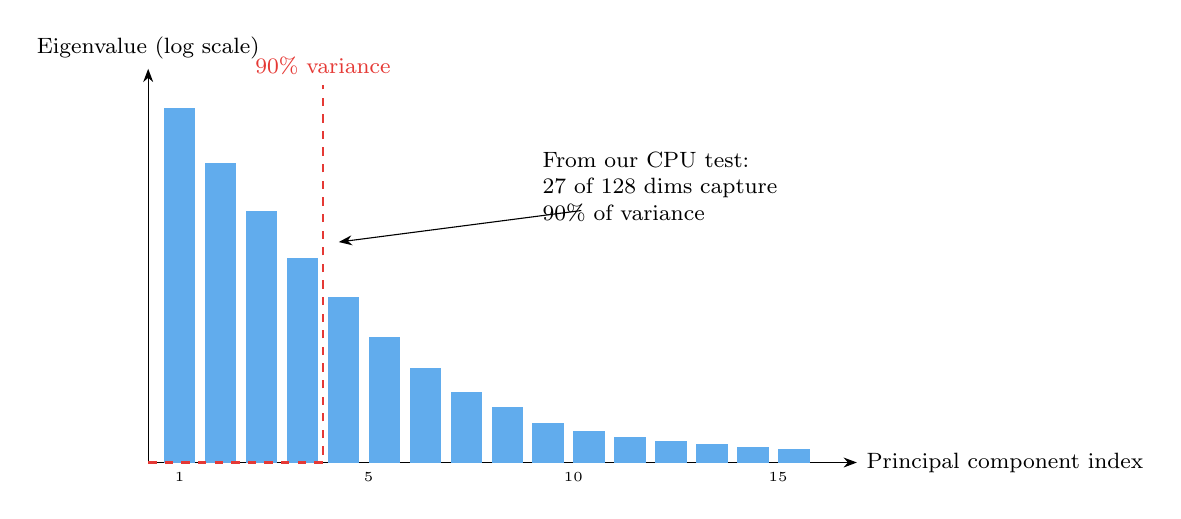
\begin{tikzpicture}[>=Stealth, font=\small]
    % Axes
    \draw[->] (0, 0) -- (9, 0) node[right, font=\footnotesize] {Principal component index};
    \draw[->] (0, 0) -- (0, 5) node[above, font=\footnotesize] {Eigenvalue (log scale)};

    % Eigenvalue bars (rapid dropoff)
    \foreach \i/\h in {0/4.5, 1/3.8, 2/3.2, 3/2.6, 4/2.1, 5/1.6, 6/1.2, 7/0.9, 8/0.7, 9/0.5, 10/0.4, 11/0.32, 12/0.27, 13/0.23, 14/0.2, 15/0.17}{
        \fill[orbitblue!70] (\i*0.52+0.2, 0) rectangle (\i*0.52+0.6, \h);
    }

    % 90% line
    \draw[dashed, seedred, thick] (0, 0) -- (3.5*0.52+0.4, 0) -- (3.5*0.52+0.4, 4.8);
    \node[seedred, font=\footnotesize, above] at (3.5*0.52+0.4, 4.8) {90\% variance};

    % Annotation
    \node[font=\footnotesize, align=left] at (6.5, 3.5) {From our CPU test:\\27 of 128 dims capture\\90\% of variance};
    \draw[->] (5.5, 3.2) -- (3.5*0.52+0.6, 2.8);

    % Axis ticks
    \node[font=\tiny, below] at (0.4, 0) {1};
    \node[font=\tiny, below] at (2.8, 0) {5};
    \node[font=\tiny, below] at (5.4, 0) {10};
    \node[font=\tiny, below] at (8.0, 0) {15};
\end{tikzpicture}
\caption{\textbf{Eigenvalue spectrum of a trained embedding matrix.}
The eigenvalues drop off rapidly: in our CPU experiments, 27 out of 128 dimensions capture 90\% of the variance.
This means the embedding table has far fewer effective degrees of freedom than $V \times d$.}
\label{fig:eigenvalues}
\end{figure}

\subsection{Why: Shared Structure}

The reason for this redundancy is simple: tokens share structure.
``Cat'' and ``dog'' are both animals.
``Run'' and ``jump'' are both verbs.
``Blue'' and ``red'' are both colours.
Each group shares a common subspace, and the embedding table stores this shared structure \emph{independently for every token}.
It is as if you wrote a phone book where every entry repeated the country code, area code, and exchange---instead of writing them once at the top of the page.

\subsection{SVD: Linear Compression}

The simplest compression is \textbf{Singular Value Decomposition}:
\[
    E \approx U_k \Sigma_k V_k^\top
\]
where $k \ll d$.
This replaces the $V \times d$ table with a $V \times k$ matrix and a $k \times d$ matrix: total $V k + k d$ parameters.
If $k = 27$ and $d = 128$, this is a $\sim 5\times$ compression.

SVD is optimal for \emph{linear} structure.
But real embeddings have nonlinear structure: tokens cluster on curved manifolds, not flat subspaces.

\subsection{The Limit of Linear}

Consider 100 points arranged in a circle in 2D.
PCA tells you the data is ``two-dimensional''---the eigenvalues are roughly equal.
No linear compression helps.
But the circle is a \emph{one-dimensional} manifold: each point is determined by a single angle $\theta$.
A nonlinear function $f(\theta) = (\cos\theta, \sin\theta)$ compresses 200 numbers (100 $\times$ 2) into 100 numbers (100 angles) plus a tiny function.
This is the gap that orbital embeddings exploit.

\paragraph{What this means in language.}
In language, the shared structure is semantic: ``cat'', ``dog'', ``bird'' all share ANIMAL features.
``Ran'', ``jumped'', ``walked'' all share ACTION features.
PCA captures these broad categories in the top components.
The redundancy is real: a 50K-token embedding table stores the ANIMAL pattern 1000+ times (once per animal word) instead of once.


% ======================================================================
\section{Functions as Replacements for Lookup}
\label{sec:functions}

\subsection{The Key Idea}

Instead of storing a vector $\mathbf{e}_w = E[w]$ for each token, compute it:
\[
    \mathbf{e}_w = f(\s_w)
\]
where $\s_w$ is a tiny \textbf{seed} (much smaller than $\mathbf{e}_w$) and $f$ is a \textbf{shared function} (the same for all tokens).

The seeds are stored per token (like a compressed address).
The function is stored once and reused for all tokens.
If the function is small relative to the savings from compression, we win.

\subsection{Universal Approximation: Any Lookup Can Be Computed}

\begin{proposition}[Function replacement]
For any finite set of target vectors $\{\mathbf{e}_1, \ldots, \mathbf{e}_V\} \subset \R^d$ and any $\epsilon > 0$, there exists a neural network $f: \R^{d_s} \to \R^d$ and seed vectors $\{\s_1, \ldots, \s_V\} \subset \R^{d_s}$ such that $\|f(\s_w) - \mathbf{e}_w\| < \epsilon$ for all $w$.
\end{proposition}

\begin{proof}[Proof sketch.]
Pick $d_s = 1$ and assign each token a unique scalar $s_w = w/V$.
By the universal approximation theorem, a sufficiently wide MLP can interpolate any finite set of points.
\end{proof}

The existence is trivial.
The interesting question is \textbf{efficiency}: when does $f$ use fewer parameters than the table it replaces?

\subsection{Concrete Example: Eight Points on a Circle}

\begin{figure}[h]
\centering
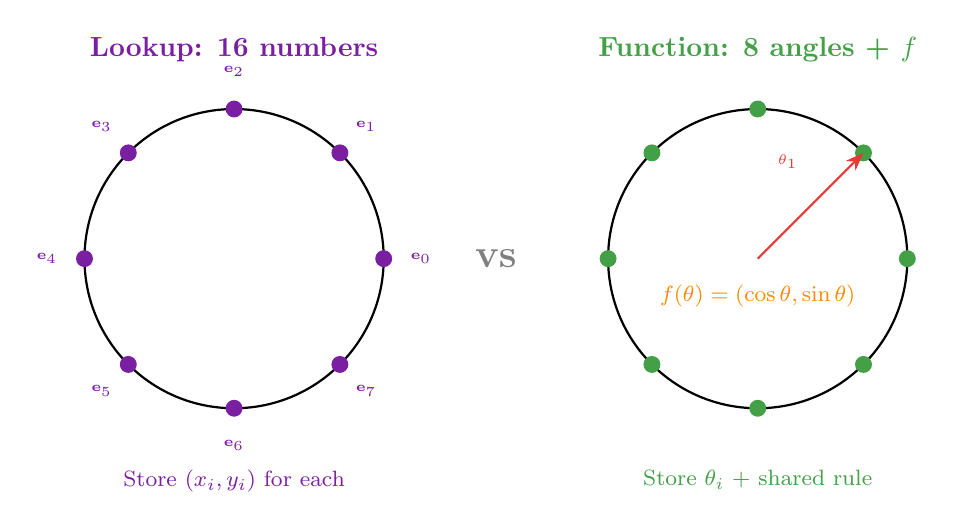
\begin{tikzpicture}[>=Stealth, font=\small, scale=0.95]
    % ── LEFT: LOOKUP ──────────────────────────────────────────────────
    \begin{scope}[shift={(-3.5, 0)}]
        \node[font=\bfseries, lookuppurple] at (0, 2.8) {Lookup: 16 numbers};
        \draw[thick] (0, 0) circle (2);
        \foreach \i in {0,...,7}{
            \pgfmathsetmacro{\angle}{45*\i}
            \pgfmathsetmacro{\px}{2*cos(\angle)}
            \pgfmathsetmacro{\py}{2*sin(\angle)}
            \filldraw[lookuppurple] (\px, \py) circle (3pt);
            \node[font=\tiny, lookuppurple] at ({2.5*cos(\angle)}, {2.5*sin(\angle)}) {$\mathbf{e}_{\i}$};
        }
        \node[font=\footnotesize, lookuppurple, below] at (0, -2.7) {Store $(x_i, y_i)$ for each};
    \end{scope}

    % ── VS ────────────────────────────────────────────────────────────
    \node[font=\Large\bfseries, gray] at (0, 0) {vs};

    % ── RIGHT: FUNCTION ───────────────────────────────────────────────
    \begin{scope}[shift={(3.5, 0)}]
        \node[font=\bfseries, targetgreen] at (0, 2.8) {Function: 8 angles + $f$};
        \draw[thick] (0, 0) circle (2);
        \foreach \i in {0,...,7}{
            \pgfmathsetmacro{\angle}{45*\i}
            \pgfmathsetmacro{\px}{2*cos(\angle)}
            \pgfmathsetmacro{\py}{2*sin(\angle)}
            \filldraw[targetgreen] (\px, \py) circle (3pt);
        }
        % Show seed arrow for one point
        \draw[->, thick, seedred] (0, 0) -- ({2*cos(45)}, {2*sin(45)});
        \node[font=\tiny, seedred] at (0.4, 1.3) {$\theta_1$};

        % Function label
        \node[font=\footnotesize, dynamicsorange] at (0, -0.5) {$f(\theta) = (\cos\theta, \sin\theta)$};
        \node[font=\footnotesize, targetgreen, below] at (0, -2.7) {Store $\theta_i$ + shared rule};
    \end{scope}
\end{tikzpicture}
\caption{\textbf{Lookup vs.\ function for eight points on a circle.}
\textbf{Left:} store all 16 coordinates (2 per point).
\textbf{Right:} store 8 angles (1 per point) and the shared function $f(\theta) = (\cos\theta, \sin\theta)$.
The function version stores 8 numbers plus a tiny function; the lookup stores 16 numbers.
The savings grow with the number of points.}
\label{fig:circle-example}
\end{figure}

\subsection{When Functions Win and When They Lose}

\begin{figure}[h]
\centering
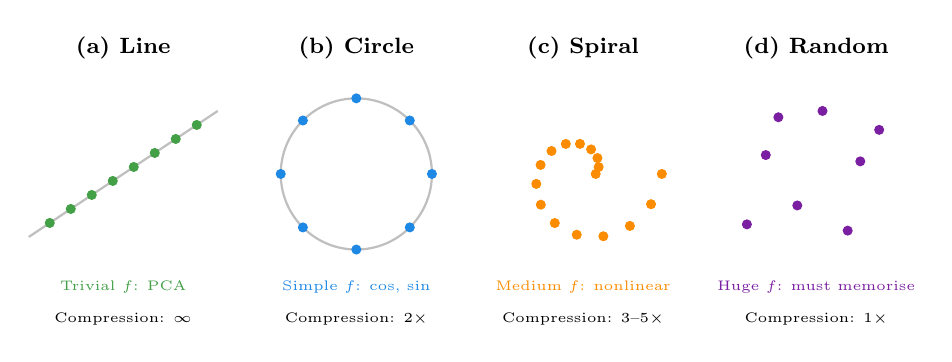
\begin{tikzpicture}[>=Stealth, font=\small, scale=0.8]
    % ── (a) Line ──────────────────────────────────────────────────────
    \begin{scope}[shift={(-5.5, 0)}]
        \node[font=\bfseries\footnotesize] at (0, 2) {(a) Line};
        \draw[gray!50, thick] (-1.5, -1) -- (1.5, 1);
        \foreach \i in {1,...,8}{
            \pgfmathsetmacro{\px}{-1.5 + 3*\i/9}
            \pgfmathsetmacro{\py}{-1 + 2*\i/9}
            \filldraw[targetgreen] (\px, \py) circle (2pt);
        }
        \node[font=\tiny, targetgreen] at (0, -1.8) {Trivial $f$: PCA};
        \node[font=\tiny] at (0, -2.3) {Compression: $\infty$};
    \end{scope}

    % ── (b) Circle ────────────────────────────────────────────────────
    \begin{scope}[shift={(-1.8, 0)}]
        \node[font=\bfseries\footnotesize] at (0, 2) {(b) Circle};
        \draw[gray!50, thick] (0, 0) circle (1.2);
        \foreach \i in {0,...,7}{
            \pgfmathsetmacro{\angle}{45*\i}
            \filldraw[orbitblue] ({1.2*cos(\angle)}, {1.2*sin(\angle)}) circle (2pt);
        }
        \node[font=\tiny, orbitblue] at (0, -1.8) {Simple $f$: $\cos$, $\sin$};
        \node[font=\tiny] at (0, -2.3) {Compression: $2\times$};
    \end{scope}

    % ── (c) Spiral ────────────────────────────────────────────────────
    \begin{scope}[shift={(1.8, 0)}]
        \node[font=\bfseries\footnotesize] at (0, 2) {(c) Spiral};
        \foreach \i in {0,...,15}{
            \pgfmathsetmacro{\angle}{24*\i}
            \pgfmathsetmacro{\rad}{0.2 + 0.07*\i}
            \filldraw[dynamicsorange] ({\rad*cos(\angle)}, {\rad*sin(\angle)}) circle (2pt);
        }
        \node[font=\tiny, dynamicsorange] at (0, -1.8) {Medium $f$: nonlinear};
        \node[font=\tiny] at (0, -2.3) {Compression: $3\text{--}5\times$};
    \end{scope}

    % ── (d) Random ────────────────────────────────────────────────────
    \begin{scope}[shift={(5.5, 0)}]
        \node[font=\bfseries\footnotesize] at (0, 2) {(d) Random};
        % Pseudo-random points
        \filldraw[lookuppurple] (-0.8, 0.3) circle (2pt);
        \filldraw[lookuppurple] (0.5, -0.9) circle (2pt);
        \filldraw[lookuppurple] (1.0, 0.7) circle (2pt);
        \filldraw[lookuppurple] (-0.3, -0.5) circle (2pt);
        \filldraw[lookuppurple] (0.7, 0.2) circle (2pt);
        \filldraw[lookuppurple] (-1.1, -0.8) circle (2pt);
        \filldraw[lookuppurple] (0.1, 1.0) circle (2pt);
        \filldraw[lookuppurple] (-0.6, 0.9) circle (2pt);
        \node[font=\tiny, lookuppurple] at (0, -1.8) {Huge $f$: must memorise};
        \node[font=\tiny] at (0, -2.3) {Compression: $1\times$};
    \end{scope}
\end{tikzpicture}
\caption{\textbf{Four geometries and their compressibility.}
(a) Points on a line: one parameter per point, trivial function.
(b) Points on a circle: one angle per point, simple trigonometric function.
(c) Points on a spiral: one parameter per point, nonlinear function.
(d) Random points: incompressible---the function must memorise every point.
Natural language embeddings are closer to (b) and (c) than to (d): they have structure that a shared function can exploit.}
\label{fig:four-geometries}
\end{figure}

Functions win when the targets have \textbf{structure}---when they lie on a low-dimensional manifold.
Functions lose when the targets are \textbf{random}---when every point is independent and there is nothing to share.

From our CPU theory tests: structured embedding targets (like circle, spiral, clustered) require only $\sim$38 parameters in the shared function to achieve 0.985 cosine similarity.
Random targets require $>$66,000 parameters---worse than just storing the table.
Natural language embeddings have real structure (our PCA tests show 90\% variance in 27/128 dimensions), so the function approach works.

\paragraph{In TinyStories\ldots}
Animal words form a manifold (smooth variation within a category).
The function $f$ learns ``what ANIMAL means'' (the manifold shape) and each seed says ``which animal'' (position on the manifold).
Random words with no shared structure---like punctuation vs content words---cannot be compressed this way and may need the sparse lookup (Section~\ref{sec:future}).


% ======================================================================
\section{Orbits: Iterated Shared Dynamics}
\label{sec:orbits}

\subsection{Why Iterate?}

A single function $f(\s_w)$ might need to be very wide to map tiny seeds to high-dimensional embeddings.
A narrow function applied \emph{multiple times} can achieve the same expressiveness with far fewer parameters.
This is the depth-vs-width tradeoff: depth (iteration) is more parameter-efficient than width for most structured functions.

\subsection{The Orbit}

An orbital embedding works in three stages:
\begin{enumerate}[nosep]
    \item \textbf{Seed lookup}: fetch a tiny vector $\s_w \in \R^{d_s}$ for token $w$ (like an address).
    \item \textbf{Projection}: map the seed into model space: $\x_0 = W_{\text{proj}} \s_w + \mathbf{b}$.
    \item \textbf{Iteration}: apply the shared dynamics $T$ times:
    \[
        \x_{t+1} = \x_t + \Phi(\x_t), \qquad t = 0, 1, \ldots, T{-}1
    \]
    where $\Phi$ is a small neural network (the same at every step).
\end{enumerate}
The final $\x_T$ is the embedding vector that replaces $E[w]$.

\begin{figure}[h]
\centering
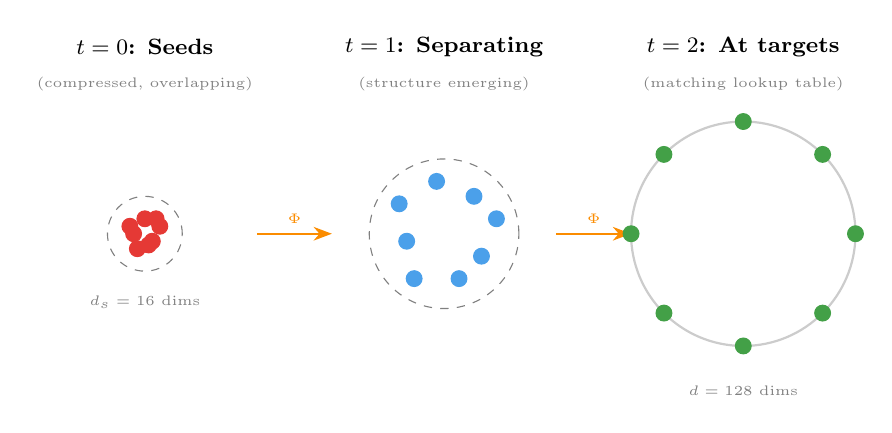
\begin{tikzpicture}[>=Stealth, font=\small, scale=0.95]
    % ── T=0: Seeds (compressed) ──────────────────────────────────────
    \begin{scope}[shift={(-4, 0)}]
        \node[font=\bfseries\footnotesize] at (0, 2.5) {$t = 0$: Seeds};
        \node[font=\tiny, gray] at (0, 2.0) {(compressed, overlapping)};

        % Cluster of seeds (tight)
        \filldraw[seedred] (-0.2, 0.1) circle (3pt);
        \filldraw[seedred] (0.1, -0.1) circle (3pt);
        \filldraw[seedred] (0.0, 0.2) circle (3pt);
        \filldraw[seedred] (-0.1, -0.2) circle (3pt);
        \filldraw[seedred] (0.2, 0.1) circle (3pt);
        \filldraw[seedred] (-0.15, 0.0) circle (3pt);
        \filldraw[seedred] (0.05, -0.15) circle (3pt);
        \filldraw[seedred] (0.15, 0.2) circle (3pt);

        \draw[gray, dashed] (0, 0) circle (0.5);
        \node[font=\tiny, gray, below] at (0, -0.7) {$d_s = 16$ dims};
    \end{scope}

    % Arrow
    \draw[->, thick, dynamicsorange] (-2.5, 0) -- (-1.5, 0) node[midway, above, font=\tiny] {$\Phi$};

    % ── T=1: After one iteration ─────────────────────────────────────
    \begin{scope}[shift={(0, 0)}]
        \node[font=\bfseries\footnotesize] at (0, 2.5) {$t = 1$: Separating};
        \node[font=\tiny, gray] at (0, 2.0) {(structure emerging)};

        % Points spreading out
        \filldraw[orbitblue!80] (-0.6, 0.4) circle (3pt);
        \filldraw[orbitblue!80] (0.5, -0.3) circle (3pt);
        \filldraw[orbitblue!80] (-0.1, 0.7) circle (3pt);
        \filldraw[orbitblue!80] (-0.4, -0.6) circle (3pt);
        \filldraw[orbitblue!80] (0.7, 0.2) circle (3pt);
        \filldraw[orbitblue!80] (-0.5, -0.1) circle (3pt);
        \filldraw[orbitblue!80] (0.2, -0.6) circle (3pt);
        \filldraw[orbitblue!80] (0.4, 0.5) circle (3pt);

        \draw[gray, dashed] (0, 0) circle (1.0);
    \end{scope}

    % Arrow
    \draw[->, thick, dynamicsorange] (1.5, 0) -- (2.5, 0) node[midway, above, font=\tiny] {$\Phi$};

    % ── T=2: At targets ──────────────────────────────────────────────
    \begin{scope}[shift={(4, 0)}]
        \node[font=\bfseries\footnotesize] at (0, 2.5) {$t = 2$: At targets};
        \node[font=\tiny, gray] at (0, 2.0) {(matching lookup table)};

        % Points on circle (final positions)
        \draw[gray!40, thick] (0, 0) circle (1.5);
        \foreach \i in {0,...,7}{
            \pgfmathsetmacro{\angle}{45*\i}
            \filldraw[targetgreen] ({1.5*cos(\angle)}, {1.5*sin(\angle)}) circle (3pt);
        }

        \node[font=\tiny, gray, below] at (0, -1.9) {$d = 128$ dims};
    \end{scope}
\end{tikzpicture}
\caption{\textbf{Orbit unfolding.}
Seeds start compressed in $\R^{d_s}$ (left).
After one iteration of $\Phi$, they begin to separate (middle).
After two iterations, they reach their target positions---matching what the lookup table would have stored (right).
The shared dynamics $\Phi$ sculpt all tokens simultaneously.}
\label{fig:orbit-unfolding}
\end{figure}

\paragraph{In TinyStories\ldots}
The orbital unfolding might work like this: at $T = 0$, the seed says ``this is token \#347'' (compressed identity).
After projection, it enters a 64-dimensional space.
After $\Phi^1$, the dynamics separate it into broad categories: ``this is an animal word'' vs ``this is an action word.''
After $\Phi^2$, within-category refinement: ``this is specifically \emph{cat}, not \emph{dog}.''
The hierarchy of the unfolding mirrors the hierarchy of semantic structure.

\subsection{Weight Sharing Across Depth}

The critical feature is that $\Phi$ is the \emph{same} at every iteration.
This is \textbf{weight sharing across depth}---the same idea used in:
\begin{itemize}[nosep]
    \item \textbf{Deep Equilibrium Models} (Bai et al., 2019): iterate one layer to convergence instead of stacking $L$ different layers.
    \item \textbf{Universal Transformers} (Dehghani et al., 2018): apply the same transformer block $T$ times with shared weights.
    \item \textbf{Recurrent neural networks}: the same cell at every time step.
\end{itemize}
All exploit the same principle: if the transformation at each step is approximately the same, share the parameters and iterate.

\begin{remark}
\textbf{Realisation: ``Generators not trajectories'' (\#9).}
A transformer stores $L$ copies of coupling patterns (trajectories).
The ORN discovers the law that generates them all (a generator) and stores it once.
This is the philosophical core of the entire programme: states vs dynamics, KV cache vs semigroup, lookup vs computation.
\end{remark}

But the ORN shares \emph{differently} from all of these.
ALBERT~\cite{lan2020albert}, Universal Transformers~\cite{dehghani2018universal}, and DEQs~\cite{bai2019deep} share \emph{everything}---every weight is identical at every layer.
The ORN shares \emph{only the coupling geometry} ($A$, $B$ --- the matrices that determine which tokens attend to which) and keeps the response heads ($W_V$, $W_O$, FFN) \textbf{per-layer}.
Recently, Meta's Relaxed Recursive Transformers~\cite{relaxedrecursive2025} confirmed this decomposition: sharing all weights + per-layer LoRA corrections recovers 99.7\% of Gemma 2B quality, validating the ``share the invariant, adapt the rest'' principle.

Why does this matter?
The per-layer response heads serve a dual role:
\begin{enumerate}[nosep]
    \item They extract content from the coupling pattern (their primary job).
    \item They \textbf{rotate the residual field} so that the next application of the same $A$, $B$ produces a different coupling pattern (an emergent side effect).
\end{enumerate}

This rotation is why the ORN's semigroup is rich---one coupling rule in $L$ different rotated frames produces $L$ distinct coupling patterns.
ALBERT cannot do this: its shared response heads produce the same rotation at every layer, so the field barely evolves and the coupling patterns barely vary.
That is why ALBERT loses ${\sim}1.5\%$ and the ORN does not.

Our spectral universality study confirms this is the right split: across five pretrained models (GPT-2, SmolLM2, Qwen2.5), the coupling geometry IS invariant (eigenvalue correlation $0.97$) while the orientation varies.
The per-layer response heads provide exactly the degrees of freedom needed---rotation---while the coupling shape is shared.

\begin{intuition}
\textbf{Realisation: One M captures 95.8\% of GPT-2's attention (\#88).}
We extracted $W_Q^\top W_K$ from every layer of GPT-2, fitted a single $\M$, and it recovered nearly all attention scores.
At GPT-2 Large, this rises to 99\%.
The coupling redundancy is real, measurable, and \emph{grows with scale}~\cite{masa2025}.
The transformer stores $L$ rotated copies of one geometric rule.
The ORN stores the rule once.
\end{intuition}

\subsection{Parameter Comparison}

\begin{center}\small
\begin{tabular}{@{}p{3.5cm}p{4cm}p{4.5cm}@{}}
\toprule
\textbf{Method} & \textbf{Parameters} & \textbf{Notes} \\
\midrule
Lookup table & $V \times d$ & No sharing, no computation \\
Single MLP & $V \times d_s + |\text{MLP}|$ & MLP may need huge width \\
\textbf{Orbital (ours)} & $V \times d_s + |\Phi|$ & $\Phi$ is small, iterated $T$ times \\
\bottomrule
\end{tabular}
\end{center}

For $V = 50{,}257$, $d = 128$, $d_s = 16$:
\begin{itemize}[nosep]
    \item Lookup: $50{,}257 \times 128 = 6.4$M parameters.
    \item Orbital ($d_s = 16$, $|\Phi| \approx 40$K): $50{,}257 \times 16 + 40{,}000 = 844$K parameters.
    \item Compression ratio: $\mathbf{7.6\times}$.
\end{itemize}

\subsection{Concrete Numbers from Our Experiments}

In our Level~0 theory tests, orbital embeddings with $T = 2$ iterations achieve:
\begin{itemize}[nosep]
    \item \textbf{0.985 cosine similarity} to the original embedding table at $2\times$ compression.
    \item \textbf{0.96 cosine similarity} at $4\times$ compression.
    \item The shared block $\Phi$ has only $\sim$40K parameters, reused at every step.
\end{itemize}
The savings are real and measurable.


% ======================================================================
\section{Breakout: Understanding Orbital Iterations}
\label{sec:breakout-iterations}
% ======================================================================

Before we proceed to the geometry theory, it is worth pausing to build
visual intuition for what happens during orbital iteration.
The key claim is simple but subtle:

\begin{quote}
\textbf{The metric tensor $\M = AB^\top$ is fixed across all iterations.
It stores the geometry of a coupling landscape, not representations.
When the field (residual stream) evolves through this landscape,
different functional couplings activate at different depths---even though
$\M$ never changes.}
\end{quote}

This section provides three demonstrations, all generated from toy
systems that isolate the orbital mechanism without the complexity of a
full language model.

% ── 5.1: Same M, Different Coupling ──────────────────────────────────
\subsection{Same M, Different Coupling at Every Depth}

Consider a fixed matrix $\M \in \R^{d \times d}$ with non-trivial
spectral structure (a few dominant singular values, many near-zero).
We start with $N$ random seed vectors and iterate:
\[
    \mathbf{h}_{t+1} = \text{LayerNorm}\bigl(\mathbf{h}_t + \alpha\,\tanh(\mathbf{h}_t \M)\bigr)
\]
At each iteration, we compute the \emph{asymmetric} coupling between
tokens---the attention pattern that $\M$ would produce:
\[
    \text{Attn}(i \to j) = \text{softmax}_j\!\Bigl(\frac{(\mathbf{h}_i A)(\mathbf{h}_j B)^\top}{\sqrt{d}}\Bigr)
\]
This is \emph{not} symmetric: token $i$'s coupling to token $j$ differs
from $j$'s coupling to $i$, exactly as in the real SharedM architecture.

\begin{figure}[h]
\centering
\includegraphics[width=\textwidth]{orbit_geometry.png}
\caption{\textbf{Same $\M$, different coupling at every depth.}
Top row: the asymmetric coupling matrix at seed, iteration~2,
iteration~5, and iteration~8. The pattern visibly changes at each
depth even though $\M$ is fixed. Bottom left: token orbits in PCA
space---seeds start clustered and separate through iteration.
Bottom centre-left: the most dynamic token pairs, showing coupling
that shifts or reverses across iterations. Bottom centre-right:
Frobenius distance of the coupling matrix from the seed---the
coupling evolves then begins to stabilise (orbit convergence).
\emph{All produced by the same fixed $\M$.}}
\label{fig:orbit-geometry}
\end{figure}

The coupling heatmaps make the claim vivid: at seed, the attention
pattern is nearly uniform (no structure). By iteration~5, specific
token pairs have developed strong directional coupling. By iteration~8,
the pattern has matured further---but it is \emph{different} from
iteration~5. The same $\M$ produced all four matrices. The only thing
that changed was the field state $\mathbf{h}$.

\begin{intuition}
Think of $\M$ as a fixed crystal. A light ray (the token state) enters
at some angle (the seed). Each pass through the crystal refracts it
differently, because the ray's angle changes after each pass. After
enough passes, the rays have been sorted by the crystal's geometry.
The crystal never changed---the light travelled through it.
\end{intuition}


% ── 5.2: The Orbit Animation ─────────────────────────────────────────
\subsection{Watching a Single Token's Orbit}

To make the iteration concrete, we track a single token $\alpha$ through
10 iterations of $\M$. At each step we record three things:

\begin{enumerate}[nosep]
    \item \textbf{Position in phase space} (PCA projection of the $d$-dimensional state vector).
    \item \textbf{Coupling pattern} (which other tokens does $\alpha$ attend to?).
    \item \textbf{State vector} (all $d$ activation values).
\end{enumerate}

\begin{figure}[h]
\centering
\begin{minipage}{0.32\textwidth}
    \centering
    \includegraphics[width=\textwidth]{frames/frame_00.png}
\end{minipage}
\hfill
\begin{minipage}{0.32\textwidth}
    \centering
    \includegraphics[width=\textwidth]{frames/frame_05.png}
\end{minipage}
\hfill
\begin{minipage}{0.32\textwidth}
    \centering
    \includegraphics[width=\textwidth]{frames/frame_10.png}
\end{minipage}
\caption{\textbf{Three frames from the orbit animation}
(full animation: \texttt{orbit\_animation.gif}).
\emph{Left}: Iteration~0 (seed). $\alpha$ is in a random position; no
coupling yet. \emph{Centre}: Iteration~5. $\alpha$ has moved through
$\M$'s geometry; strong coupling to $\delta$ has emerged.
\emph{Right}: Iteration~10. $\alpha$ has reached a different region;
coupling has shifted---$\alpha$ now couples to itself and $\varepsilon$
in addition to $\delta$. Same $\M$ at every step.}
\label{fig:orbit-animation}
\end{figure}

The critical observation: $\alpha$'s coupling partners \emph{change}
across iterations. At iteration~5, it attends almost exclusively to
$\delta$. By iteration~10, the attention has redistributed. In a trained
language model, this is how the same shared $\M$ produces
determiner$\to$noun coupling at one depth and noun$\to$verb coupling at another.
Functional role is not stored in the embedding---it is a
\emph{phase of the orbit}.


% ── 5.3: Reachability ────────────────────────────────────────────────
\subsection{Reachability: The Semigroup Image}
\label{sec:breakout-reachability}

If $\M$ defines the geometry, what constrains the set of states that
iteration can reach? This is the question of \textbf{reachability}---the
image of the semigroup generated by $\M$.

We initialise 50 random seeds in $\R^d$ and iterate all of them through
the same $\M$. Figure~\ref{fig:reachability} shows the result.

\begin{figure}[h]
\centering
\includegraphics[width=\textwidth]{reachability.png}
\caption{\textbf{$\M$'s semigroup constrains the orbit space.}
Top row: 50 random seeds at iterations 0, 2, 5, 10---the cloud
contracts onto a lower-dimensional manifold. Bottom left: effective
dimensionality (participation ratio of singular values) drops from
$\sim$14 to $\sim$4, matching $\M$'s 5 significant singular values.
Bottom centre: $\M$'s spectrum---the number of large singular values
defines the orbit manifold dimension.}
\label{fig:reachability}
\end{figure}

This is the \textbf{capacity} of the semigroup. A metric tensor $\M$
with $k$ significant singular values can support orbits that live on a
$\sim$$k$-dimensional manifold. More iterations compress the reachable
set further onto $\M$'s dominant subspace. This means:

\begin{itemize}[nosep]
    \item The \textbf{rank of $\M$} bounds the expressiveness of the orbits.
    \item The \textbf{number of iterations $L$} determines how tightly
      states are compressed onto the dominant manifold.
    \item A \textbf{low-rank $\M$} forces all tokens onto a small subspace
      (not enough capacity). A \textbf{full-rank $\M$} preserves all
      directions but may not develop useful structure.
    \item The sweet spot: $\M$ with a \emph{few dominant and many
      suppressed} singular values creates a structured manifold where
      functional roles emerge as regions.
\end{itemize}

The effective dimensionality after $L$ iterations is an empirical
diagnostic for whether $\M$ has learned useful geometry: if it collapses
to 1--2 dimensions, $\M$ is degenerate; if it stays at $d$, $\M$ has
not learned to compress; a value in between (say 5--15 for $d = 128$)
suggests structured, useful orbits.


% ── 5.4: Context Steering ────────────────────────────────────────────
\subsection{Context Steering: Same Seed, Different Orbit}

In a full SharedM model, the orbit of a token depends not only on its
seed but on the \emph{context}---the other tokens in the sequence.
At each iteration, the value projections $W_V$ (per-layer) and the
feed-forward network inject context-dependent information through the
coupling that $\M$ defines.

\begin{itemize}[nosep]
    \item $\M$ determines \emph{who} attends to \emph{whom} (the coupling geometry).
    \item $W_V$ determines \emph{what information} flows through that coupling.
    \item Context (surrounding tokens) modulates what is available to flow.
\end{itemize}

$\M$ is the river. Context is the rudder.

\begin{figure}[h]
\centering
\includegraphics[width=\textwidth]{context_steering.png}
\caption{\textbf{Context steering}: Same seed token $\alpha$, same $\M$,
three different context signals $\to$ three different orbits.
Top row: each panel shows $\alpha$'s orbit under a different context.
Bottom left: overlay of all three---same start point ($\star$),
different endpoints (squares).
\textbf{Bottom centre (key panel)}: $\alpha$'s coupling pattern at
mid-depth, shown for all three contexts. These bar charts are
analogous to a single row of the $QK^\top$ coupling matrix in a
standard transformer---the attention distribution that determines
what information flows to $\alpha$. In a standard transformer, each
layer stores its own $W_Q, W_K$ to produce this pattern. In SharedM,
the \emph{same} $\M = AB^\top$ is driven for $L$ iterations by the
semigroup it generates, and the resulting coupling matrix emerges
from the interaction of $\M$'s fixed geometry with the evolving
field. The semigroup's capacity---the dimensionality of its
image after $L$ steps---determines how rich and varied these
coupling patterns can be (Section~\ref{sec:breakout-reachability}).}
\label{fig:context-steering}
\end{figure}

This is why ``cat'' in ``the cat sat'' ends up in a different region of
representation space than ``cat'' in ``a cat ran on a mat''. The seed is
the same. The metric tensor is the same. But the surrounding context
steers the orbit to a different destination through $\M$'s geometry.

\paragraph{The coupling matrix is not stored---it is computed.}
In a standard transformer, each layer independently stores
$W_Q^{(\ell)}, W_K^{(\ell)} \in \R^{d \times d}$, giving $2Ld^2$
coupling parameters across $L$ layers. Each layer's coupling matrix
$Q^{(\ell)}{K^{(\ell)}}^\top$ is a separate, independently learned
pattern. In SharedM, there is a single $\M = AB^\top$ shared across
all layers. The coupling matrix at layer $\ell$ is:
\[
    \text{Attn}^{(\ell)} = \text{softmax}\!\Bigl(
        \frac{(\mathbf{h}^{(\ell)} A)(\mathbf{h}^{(\ell)} B)^\top}{\sqrt{d_h}}
    \Bigr)
\]
where $\mathbf{h}^{(\ell)}$ is the residual stream at depth $\ell$.
Because $\mathbf{h}^{(\ell)}$ differs at every layer (the field has
been updated by all previous iterations), $\M$ produces a
\emph{different} $\text{Attn}^{(\ell)}$ at each depth---despite being
the same matrix. The coupling patterns in the bottom-centre panel of
Figure~\ref{fig:context-steering} are three instances of this: same
$\M$, different field states (due to different contexts), different
resulting attention distributions.

The parameter saving is $2Ld^2 \to 2d^2$ for coupling, an
$L$-fold compression. But the \emph{capacity} of the resulting
coupling is not merely $d^2$---it is determined by the semigroup
generated by $\M$ over $L$ iterations. Each iteration drives the field
to a new region of $\M$'s geometry, producing a coupling matrix that
could not have been produced at any other depth. The semigroup's image
after $L$ steps spans a space of coupling patterns whose dimensionality
grows with $L$, up to the capacity limit set by $\M$'s spectral
structure. Our scaling experiments (Section~\ref{sec:exp5b-results})
provide empirical evidence that this computed capacity matches or
exceeds the stored capacity of $2L$ independent projection matrices.

Context steering connects directly to the \textbf{response heads} $W_V$
in the GRF decomposition (Section~\ref{sec:orn-attention}). The
generator $\M$ defines reachable orbits; the response heads select
\emph{which} orbit to follow based on context. The reachable set from a
given seed---the fan of possible endpoints under all possible
contexts---characterises the \textbf{functional range} of that token.
A token with a large reachable set is functionally versatile (like
``set'' or ``run'' in English); one with a small reachable set is
functionally rigid (like ``the'').

\bigskip
\noindent
With this visual intuition in hand, we now show what the semigroup looks like \emph{in a real trained model}, then turn to the formal geometry that explains why shared dynamics produce useful structure.

% ──────────────────────────────────────────────────────────────────────
\subsection{From the Lab: The Semigroup at 50M Parameters}
\label{sec:semigroup-lab}

Everything above used toy examples.
Here we open a real checkpoint---SharedM-50M ($d{=}512$, $L{=}9$, trained on TinyStories for 8{,}000 steps)---and look at what $\M = AB^\top$ actually learned.

\paragraph{The probe sentence.}
We feed the model a single sentence and trace what happens at every layer:
\begin{quote}\itshape
``Once upon a time, there was a little girl named Lily. She loved to play with her dog.''
\end{quote}
(21 tokens under GPT-2 tokenization.)

\paragraph{Q-vectors rotate smoothly.}
Figure~\ref{fig:tut-orbits} (left) shows the cosine similarity between the query vector for ``dog'' at each pair of layers.
Adjacent layers have cosine ${\sim}0.9$---nearly the same query---but by layer~8 the query has rotated so far that the L0$\leftrightarrow$L8 cosine is only $0.29$.
This is the orbit: the same $A$ matrix, applied to a progressively transformed residual stream, smoothly sweeps the query through coupling space.

\paragraph{K-vectors undergo a phase transition.}
Figure~\ref{fig:tut-orbits} (centre) shows the same analysis for the key vector of ``Lily.''
The pattern is dramatically different: layers~0--3 form one cluster (cosine $0.67$--$0.97$), layers~4--8 form another ($0.70$--$0.96$), and the two clusters are nearly orthogonal (L0$\leftrightarrow$L6 $= -0.22$).
``Lily'' \emph{switches role} mid-network---from a name token to a narrative agent.
No layer-specific parameters drive this; the field state alone causes the switch.

\paragraph{Coreference emerges.}
Figure~\ref{fig:tut-coref} plots the K-vector cosine between ``Lily'' and ``She'' (co-referent) vs ``Lily'' and ``dog'' (different entity) across layers.
At deeper layers, the co-referent pair is more similar in key space than the non-co-referent pairs.
The model discovered that ``Lily'' and ``She'' should be findable by similar queries---without any coreference supervision.

\begin{figure}[h]
\centering
\includegraphics[width=\textwidth]{../experiments/results/semigroup/qk_orbits.png}
\caption{Pairwise cosine similarity of Q/K vectors across 9 layers (head~0) in a 50M-parameter SharedM model. Left: Q for ``dog'' rotates smoothly (the semigroup orbit). Centre: K for ``Lily'' shows a phase transition at layer~4. Right: K for ``She'' shows a similar phase transition, consistent with coreference.}
\label{fig:tut-orbits}
\end{figure}

\begin{figure}[h]
\centering
\includegraphics[width=0.7\textwidth]{../experiments/results/semigroup/coreference_kspace.png}
\caption{K-space cosine similarity across layers. Co-referent tokens (``Lily'' and ``She'') converge in key space, while different entities (``Lily'' vs ``dog'') diverge. Same $\M$, no coreference supervision.}
\label{fig:tut-coref}
\end{figure}

\paragraph{What the coupling geometry looks like.}
$\M$ has effective rank~51 out of 512 dimensions (90\% of energy in 51 singular values).
During training, this rank \emph{sharpens}: from 66 at step~2{,}000 to 51 at step~8{,}000.
The coupling geometry crystallises---it discovers its structure, then refines it.
This is visible in Figure~\ref{fig:tut-spectral}: the singular value spectrum concentrates into fewer, stronger modes as training progresses.

\begin{figure}[h]
\centering
\includegraphics[width=\textwidth]{../experiments/results/semigroup/spectral_evolution.png}
\caption{Left: $\M$'s singular value spectrum at four training checkpoints---energy concentrates in fewer modes over time. Right: effective rank drops from 66 to 51 while the top singular value grows. The geometry crystallises during training.}
\label{fig:tut-spectral}
\end{figure}

\paragraph{Layer specialisation from a single M.}
Figure~\ref{fig:tut-attn} shows the full attention heatmaps (head~0) at all 9 layers.
Layer~0 attends to recent context (``dog'', ``her'').
Layer~1 attends to narrative framing (``Once'', ``upon'').
Layers~6--8 attend to character identity (``Lily'', ``named'', ``girl'').
The same $\M$ produces local attention, structural attention, and entity-focused attention at different depths---driven by the field state, not by parameter diversity.

\begin{figure}[h]
\centering
\includegraphics[width=\textwidth]{../experiments/results/semigroup/attention_heatmaps.png}
\caption{Attention patterns (head~0) at all 9 layers for the same input. Same $\M$, different field state, different coupling at every depth. Early layers are local; late layers focus on character identity.}
\label{fig:tut-attn}
\end{figure}

\paragraph{The punchline.}
One $512 \times 512$ matrix pair (A, B) produces 9 distinct, semantically meaningful attention patterns.
It discovers coreference without supervision.
Its spectral structure crystallises during training, sharpening from diffuse to focused.
This is what ``generators, not trajectories'' looks like in practice.

\paragraph{A practical bonus: inspectability.}
Everything above was extracted from a single 191MB checkpoint file, with a few minutes of CPU computation.
No retraining, no ablation experiments, no evaluation datasets.

In a standard transformer, the coupling behaviour is spread across $2L$ independent $W_Q$, $W_K$ matrices---there is no single object to inspect.
In SharedM, $\M = AB^\top$ is that object.
From one checkpoint you can compute its eigenspectrum, measure its effective rank, trace how Q and K vectors orbit through layers, test what happens at depths the model was never trained on (just iterate $\M$ more times), and project the residual stream onto $\M$'s singular vectors to check whether the model is maintaining useful signal.

This makes SharedM models fundamentally more \textbf{interpretable} than standard transformers---not because the maths is simpler, but because the coupling geometry is concentrated in one place rather than distributed across layers.
The shared metric tensor is a window into the model's relational world model~\cite{brunton2022data}.

\begin{remark}
\textbf{Realisation: The value of frozen-M is interpretability, not compute savings (\#65).}
When we freeze $\M$ and train only response heads, we can watch the response heads adapt to a \emph{fixed} geometric structure.
The question changes from ``what is the model learning?'' (intractable) to ``how is the model using the geometry we already understand?'' (tractable).
At 108M parameters, the V2 model's $\M$ has effective rank 69, with 50\% of coupling energy in just 13 singular values.
These 13 modes are the model's relational grammar---the invariant coupling rules that govern how tokens relate at every layer.
\end{remark}

% ======================================================================
\section{The Geometry: Why Shared Dynamics Work}
\label{sec:geometry}

This section explains the deeper reason why a single shared function can generate all token embeddings.
The answer comes from geometry and dynamical systems theory.

\subsection{The Manifold Hypothesis}

High-dimensional data (images, text embeddings, etc.) does not fill the entire space $\R^d$.
Instead, it concentrates near low-dimensional \textbf{manifolds}---curved surfaces embedded in the high-dimensional space.

For language embeddings: $V = 50{,}000$ tokens each with a $d = 768$-dimensional vector live in a space of 768 dimensions.
But the \emph{effective} dimensionality is much lower---our PCA tests show 90\% of variance in $\sim$27 directions.
The embedding vectors lie on a $\sim$27-dimensional manifold in 768-dimensional space.

\subsection{The Dynamical System View}

The shared function $\Phi$ defines a \textbf{vector field} over the embedding space: at every point $\x$, the vector $\Phi(\x)$ says ``move this way.''
A seed $\s_w$ is an initial condition.
The orbit $\s_w \to \x_1 \to \x_2 \to \ldots$ traces a path through the space, following the vector field.
The final point is the embedding.

\begin{figure}[h]
\centering
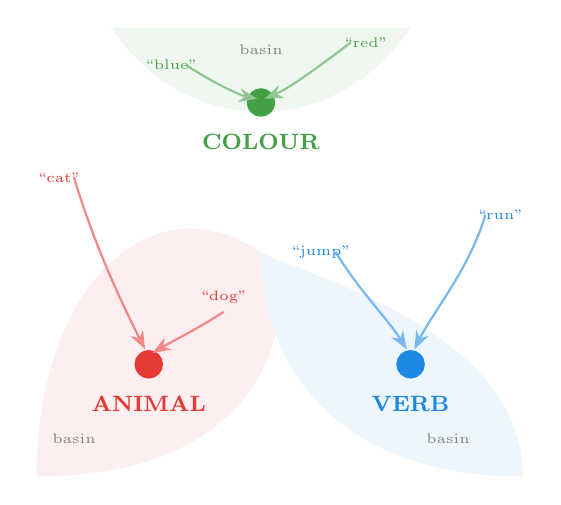
\begin{tikzpicture}[>=Stealth, font=\small, scale=0.95]
    % Background basins
    \fill[seedred!8] (-3, -2.5) .. controls (-3, 0) and (-1.5, 1.5) .. (0, 0.5) .. controls (0.5, 0.2) and (0.5, -2.5) .. (-3, -2.5);
    \fill[orbitblue!8] (0, 0.5) .. controls (0.5, 0.2) and (3.5, -0.5) .. (3.5, -2.5) .. controls (1, -2.5) and (0, -1) .. (0, 0.5);
    \fill[targetgreen!8] (-2, 3.5) .. controls (-1, 2) and (1, 2) .. (2, 3.5) -- (-2, 3.5);

    % Attractors
    \filldraw[seedred, thick] (-1.5, -1.0) circle (5pt);
    \node[font=\footnotesize\bfseries, seedred, below] at (-1.5, -1.3) {ANIMAL};

    \filldraw[orbitblue, thick] (2.0, -1.0) circle (5pt);
    \node[font=\footnotesize\bfseries, orbitblue, below] at (2.0, -1.3) {VERB};

    \filldraw[targetgreen, thick] (0.0, 2.5) circle (5pt);
    \node[font=\footnotesize\bfseries, targetgreen, below] at (0.0, 2.2) {COLOUR};

    % Trajectories into ANIMAL basin
    \draw[->, thick, seedred!60] (-2.5, 1.5) .. controls (-2.2, 0.5) and (-1.8, -0.3) .. (-1.55, -0.8);
    \node[font=\tiny, seedred] at (-2.7, 1.5) {``cat''};
    \draw[->, thick, seedred!60] (-0.5, -0.3) .. controls (-0.8, -0.5) and (-1.2, -0.7) .. (-1.45, -0.85);
    \node[font=\tiny, seedred] at (-0.5, -0.1) {``dog''};

    % Trajectories into VERB basin
    \draw[->, thick, orbitblue!60] (3.0, 1.0) .. controls (2.8, 0.3) and (2.3, -0.3) .. (2.05, -0.8);
    \node[font=\tiny, orbitblue] at (3.2, 1.0) {``run''};
    \draw[->, thick, orbitblue!60] (1.0, 0.5) .. controls (1.3, 0.0) and (1.7, -0.4) .. (1.95, -0.8);
    \node[font=\tiny, orbitblue] at (0.8, 0.5) {``jump''};

    % Trajectories into COLOUR basin
    \draw[->, thick, targetgreen!60] (-1.0, 3.0) .. controls (-0.7, 2.8) and (-0.3, 2.6) .. (-0.05, 2.55);
    \node[font=\tiny, targetgreen] at (-1.2, 3.0) {``blue''};
    \draw[->, thick, targetgreen!60] (1.2, 3.3) .. controls (0.8, 3.0) and (0.4, 2.7) .. (0.05, 2.55);
    \node[font=\tiny, targetgreen] at (1.4, 3.3) {``red''};

    % Basin labels
    \node[font=\tiny, gray] at (-2.5, -2.0) {basin};
    \node[font=\tiny, gray] at (2.5, -2.0) {basin};
    \node[font=\tiny, gray] at (0, 3.2) {basin};
\end{tikzpicture}
\caption{\textbf{Attractor landscape.}
The shared dynamics $\Phi$ define basins of attraction.
Tokens of the same semantic role (animals, verbs, colours) flow into the same basin.
Different seeds land at different points within the basin (``cat'' $\neq$ ``dog''), but the basin structure is shared.
This is why one function can generate all embeddings: it encodes the \emph{landscape}, and seeds select locations within it.}
\label{fig:attractors}
\end{figure}

\paragraph{What this means in language.}
The basins of attraction correspond to semantic roles: the ANIMAL basin, the ACTION basin, the EMOTION basin.
``Cat'' and ``dog'' have nearby seeds that flow into the same basin but settle at different positions within it.
``Cat'' and ``jumped'' have distant seeds that flow into different basins entirely.
The attractor landscape IS the learned ontology of the vocabulary.

\subsection{Contracting and Expanding Directions}

Within each basin, the dynamics have two types of directions:
\begin{description}[nosep]
    \item[Contracting directions:] tokens of the same role converge. ``Cat'' and ``dog'' share the ANIMAL subspace; the dynamics push them toward it.
    \item[Expanding directions:] tokens with different identities separate. ``Cat'' and ``dog'' are both animals but different animals; the dynamics push them apart along the identity axis.
\end{description}
This dual behaviour---contracting in some directions, expanding in others---is exactly what makes the representation rich enough for downstream processing while remaining compressible.

\subsection{Connection to the Shared Metric M}

In the broader ORN (Orbital Response Network) programme, the shared coupling tensor $\M$ solves a different problem: it replaces per-layer attention projections (Table~2 from Section~\ref{sec:two-tables}).
Where orbital embeddings ask ``can we \emph{generate} token representations from seeds?'', the shared $\M$ asks ``can we \emph{reuse} the same coupling rule at every layer?''

The two ideas connect through geometry: $\M$ defines a Riemannian metric on the residual stream (how to measure distance between tokens), and the orbital dynamics $\Phi$ operate \emph{within} this metric space (how tokens move).
The metric says ``which tokens should interact''; the dynamics say ``how their representations evolve.''
Together, they define a complete geometric system---one shared coupling rule, one shared dynamical law, and minimal per-token seeds.

\subsection{Connection to Semigroups}

The iterated dynamics have an algebraic structure: if $T(t)$ denotes $t$ iterations of $\Phi$, then:
\[
    T(s + t) = T(s) \circ T(t)
\]
This is the \textbf{semigroup property}: composing $s$ steps and $t$ steps is the same as taking $s + t$ steps.
Why does this matter?

\begin{intuition}
The semigroup property means the model learns a \emph{law}---a consistent rule of evolution---not a sequence of $T$ unrelated transforms.
If each iteration were a different function ($\Phi_1, \Phi_2, \ldots$), the model would need to learn $T$ separate rules and how they compose.
With shared $\Phi$, it learns one rule, and composition is automatic.
\end{intuition}

This is not just elegant.
Deep-OSG~\cite{chen2023deeposg} results show that enforcing semigroup structure \emph{reduces data dependency}: the model learns faster and generalises better because the search space is constrained to consistent dynamics.
The mathematical foundations are established in operator theory~\cite{brunton2022data}; the deep learning connection was first drawn by Mehta \& Schwab~\cite{mehta2014} (exact mapping between renormalisation group and deep learning) and formalised in Lin \& Tegmark~\cite{lin2017} (cheap learning works because physics has symmetries).

\subsection{The Koopman Connection: Dynamics Instead of States}

There is a deep mathematical reason why shared dynamics work, and it comes from an 80-year-old idea that was recently revived by machine learning.

\paragraph{The problem with states.}
A standard transformer stores \emph{states}: KV caches hold the key and value projections at every layer for every token.
This is memory---a snapshot of what the network computed.
If you want to extend the computation (think longer, add more context), you need more memory.
The states do not compose: knowing the KV cache at layer 5 and the KV cache at layer 10 does not tell you what the KV cache at layer 15 would be.

\paragraph{The Koopman insight: look at the dynamics, not the states.}
In 1931, B.~O.~Koopman and John von Neumann proved something remarkable: any nonlinear dynamical system can be represented as a \emph{linear} operator acting on functions of the state, rather than on the state itself.
The trick: instead of tracking $x_{t+1} = F(x_t)$ (nonlinear, hard to analyse), define the Koopman operator $\mathcal{K}$ as $\mathcal{K}[g] = g \circ F$---``apply the observable $g$ after one step of dynamics.''
$\mathcal{K}$ is linear even when $F$ is nonlinear, because composition distributes over addition: $\mathcal{K}[\alpha g + \beta h] = \alpha g \circ F + \beta h \circ F$.

The price: $\mathcal{K}$ is infinite-dimensional (the space of all functions of $x$).
The revival: machine learning can learn finite-dimensional approximations---a small matrix $K$ that captures the important dynamics.

\paragraph{M IS a Koopman approximation.}
The ORN's shared coupling matrix $\M$ is exactly this: a finite-dimensional linear operator that evolves representations through dynamics.
\begin{itemize}[nosep]
    \item The embedding layer is the \emph{encoder}: it maps tokens into the space of ``observables'' (the residual stream).
    \item $\M$ evolves observables linearly: $h_{\ell+1} \approx h_\ell + \M \cdot h_\ell$ (the residual update).
    \item The output head is the \emph{decoder}: it maps from observable space back to predictions.
    \item The response heads at each layer provide the nonlinearity that makes this approximation expressive despite $\M$ being applied linearly.
\end{itemize}

Composition is free: applying $\M$ for $s$ steps then $t$ steps IS $s{+}t$ steps.
Multi-step reasoning IS matrix powering.
The eigenvalues of $\M$ encode the \emph{timescales} of the dynamics: large eigenvalues mean fast modes (rapid prediction), small eigenvalues mean slow modes (gradual evolution, deliberation).
The eigenvectors encode the \emph{independent directions} along which dynamics decouple.

\begin{intuition}
A standard transformer stores what happened (states, KV cache).
The ORN stores how things evolve (the generator $\M$).
This is the difference between memorising a trajectory and learning the law of motion.
Given the law, you can generate any trajectory.
Given a trajectory, you can only replay it.
\end{intuition}

\paragraph{Why this matters for language.}
Language has dynamics at multiple timescales: word-to-word coupling (syntax, fast), sentence-to-sentence coupling (discourse, medium), topic-level coupling (narrative, slow).
A Koopman-style $\M$ captures all of these as different eigenmodes:
\begin{itemize}[nosep]
    \item Fast modes (large $|\lambda_i|$): local grammar, adjacent-word coupling.
    \item Medium modes: clause structure, argument binding.
    \item Slow modes (small $|\lambda_i|$): topic drift, narrative arc, long-range coherence.
\end{itemize}
All live in the same matrix.
The response heads at each layer read the relevant modes for their depth: early layers use fast modes (local syntax), deep layers use slow modes (discourse structure).
This is why $\M$ crystallises to rank ${\sim}20$ for web text: roughly 20 independent timescales capture the coupling dynamics of natural language.

\paragraph{The connection to thinking.}
The fast modes converge quickly: a few iterations through $\M$ and the prediction is sharp.
The slow modes evolve gradually: many iterations are needed to see their effect.
Fast prediction uses the fast modes (System~1).
Slow deliberation needs the slow modes (System~2).
The challenge is that prediction training---which optimises for single-step accuracy---crushes the slow modes because they don't contribute to next-token loss.
Protecting these slow Koopman modes is the key to building a system that can both predict fluently and reason deliberately, using the same $\M$ for both.


% ======================================================================
\section{A Domain Where You Can See It: Signal Processing}
\label{sec:fourier}

The best way to build intuition for orbital embeddings is to see the same idea in a domain where it is well understood: Fourier analysis.

\subsection{Fourier Series}

Any periodic signal can be decomposed into a sum of sinusoids:
\[
    f(t) = a_0 + \sum_{n=1}^{N} \left[ a_n \cos(n\omega t) + b_n \sin(n\omega t) \right]
\]
Each sinusoid is characterised by an amplitude and a phase.
The frequencies $\omega, 2\omega, 3\omega, \ldots$ are harmonics.

\subsection{Each Sinusoid Is an Orbit}

A sinusoid at frequency $\omega$ is the orbit of the \textbf{rotation operator}:
\[
    e^{i\omega t} = \cos(\omega t) + i \sin(\omega t)
\]
The ``seed'' is the complex amplitude $A_n = a_n - i b_n$ (containing amplitude and phase).
The ``dynamics'' is rotation at frequency $\omega$: multiply by $e^{i\omega \Delta t}$ at each time step.

The \textbf{shared dynamics} is rotation itself---the same operation for all frequencies.
Only the seed (amplitude, phase) and the frequency differ between components.

\subsection{The Analogy}

\begin{center}\small
\begin{tabular}{@{}lll@{}}
\toprule
& \textbf{Fourier} & \textbf{Orbital Embeddings} \\
\midrule
Stored representation & Signal samples $f(t_1), f(t_2), \ldots$ & Embedding table $E[w]$ \\
Compressed code (seed) & Fourier coefficients $(a_n, b_n)$ & Seed vectors $\s_w$ \\
Shared dynamics & Rotation: $e^{i\omega t}$ & Shared block: $\Phi$ \\
Generation & Inverse FFT & Iterate $\Phi$ on seeds \\
Structure exploited & Periodicity & Manifold structure \\
\bottomrule
\end{tabular}
\end{center}

\subsection{Concrete Example: Square Wave}

A square wave can be stored as $N$ sample values (lookup: $N$ numbers).
Or it can be represented as Fourier coefficients: a square wave with $K$ harmonics needs only $K$ coefficients, and the reconstruction formula (shared dynamics) is the same for any signal.
As $K$ grows, the approximation improves.
This is exactly the compute-vs-memory tradeoff: store the samples (memory) or store the coefficients and recompute (compute).

For natural language embeddings, the ``Fourier coefficients'' are the seeds, and the ``reconstruction formula'' is the shared block $\Phi$.
The quality of the approximation depends on how structured the target embeddings are---just as Fourier compression depends on how smooth the signal is.


% ======================================================================
\section{Building It: Orbital Embeddings in PyTorch}
\label{sec:code}

Here is the complete implementation, simplified to its essentials.

\begin{lstlisting}[caption={Orbital embedding: the complete module.}]
import torch
import torch.nn as nn

class OrbitalEmbedding(nn.Module):
    """Replace nn.Embedding(V, d) with seeds + shared dynamics."""

    def __init__(self, V, d_model, d_seed=16, T=2):
        super().__init__()
        self.T = T

        # Per-token: tiny seed vectors
        self.seeds = nn.Embedding(V, d_seed)      # V x d_seed

        # Shared: project seed -> model space
        self.proj = nn.Linear(d_seed, d_model)     # d_seed x d_model

        # Shared: the orbital dynamics (used T times)
        self.orbit = nn.Sequential(
            nn.LayerNorm(d_model),
            nn.Linear(d_model, d_model),
            nn.GELU(),
            nn.Linear(d_model, d_model),
        )

    def forward(self, token_ids):
        # Step 1: look up tiny seeds
        s = self.seeds(token_ids)      # (batch, seq) -> (batch, seq, d_seed)

        # Step 2: project into model space
        x = self.proj(s)               # (batch, seq, d_model)

        # Step 3: iterate shared dynamics T times
        for t in range(self.T):
            x = x + self.orbit(x)      # residual connection

        return x                       # (batch, seq, d_model)
\end{lstlisting}

\subsection{Line by Line}

\begin{description}
    \item[Line 11: \texttt{self.seeds}] A standard embedding table, but with $d_{\text{seed}} = 16$ instead of $d_{\text{model}} = 128$.
    This is the per-token storage: $V \times 16$ parameters instead of $V \times 128$.
    A $\mathbf{8\times}$ reduction in per-token parameters.

    \item[Line 14: \texttt{self.proj}] A single linear layer that maps the 16-dimensional seed into the 128-dimensional model space.
    Shared across all tokens.
    Cost: $16 \times 128 = 2{,}048$ parameters.

    \item[Lines 17--21: \texttt{self.orbit}] The shared dynamics block.
    LayerNorm + Linear + GELU + Linear.
    This is the ``physics'' that generates embeddings from seeds.
    Used $T$ times but stored once.
    Cost: $\sim d_{\text{model}}^2$ parameters ($\sim$40K for $d = 128$, $\sim$300K for $d = 384$).

    \item[Line 25: \texttt{self.seeds(token\_ids)}] The only per-token operation: a standard embedding lookup, but in the tiny seed space.

    \item[Line 28: \texttt{self.proj(s)}] Project from seed space to model space.
    All tokens use the same projection matrix.

    \item[Lines 31--32: \texttt{x = x + self.orbit(x)}] The orbital iteration.
    The residual connection ($x + \ldots$) ensures the iteration is stable: each step refines the previous, rather than replacing it.
    The same \texttt{self.orbit} is called $T$ times---weight sharing across depth.
\end{description}

\subsection{The Output Head}

For language modelling, the output head maps the final hidden state back to a probability distribution over tokens.
With orbital embeddings, we project back into seed space and dot with all seed vectors:

\begin{lstlisting}[caption={Output head for orbital embeddings.}]
class OrbitalOutputHead(nn.Module):
    def __init__(self, d_model, d_seed, seeds_weight):
        super().__init__()
        self.proj_out = nn.Linear(d_model, d_seed)
        self.seeds_weight = seeds_weight  # tied with input seeds

    def forward(self, hidden):
        # Project back to seed space
        z = self.proj_out(hidden)         # (batch, seq, d_seed)
        # Dot product with all seed vectors
        logits = z @ self.seeds_weight.T  # (batch, seq, V)
        return logits
\end{lstlisting}

\subsection{Parameter Counting}

\begin{center}\small
\begin{tabular}{@{}p{4cm}rr@{}}
\toprule
\textbf{Component} & \textbf{Lookup} & \textbf{Orbital ($d_s{=}16$, $T{=}2$)} \\
\midrule
Per-token storage & $V \times d = 6.4$M & $V \times d_s = 804$K \\
Projection & --- & $d_s \times d = 2$K \\
Shared dynamics ($\Phi$) & --- & $\sim 2 d^2 = 40$K \\
\midrule
\textbf{Total embedding} & \textbf{6.4M} & \textbf{846K} \\
\textbf{Compression} & $1\times$ & $\mathbf{7.6\times}$ \\
\bottomrule
\end{tabular}
\end{center}

The saved 5.5M parameters are not wasted---they are \textbf{redistributed} to make the model wider.
Instead of a model with $d = 36$ (because the embedding ate all the parameters), we get a model with $d = 128$ or higher.
The model backbone---attention layers, feed-forward networks---gets 5.5M more parameters to work with.


% ======================================================================
\section{Experiments: What We Found on TinyStories}
\label{sec:experiments}

\subsection{The Parameter Dominance Problem}

At a total budget of 2M parameters with vocabulary $V = 50{,}257$:
\begin{itemize}[nosep]
    \item The embedding table alone wants $V \times d$ parameters.
    \item If $d = 36$ (squeezed to fit): embedding = $50{,}257 \times 36 = 1.81$M = \textbf{91\% of the model}.
    \item The transformer backbone gets only 180K parameters: $d_{\text{head}} = 9$, barely functional.
\end{itemize}
The model is strangled by its own lookup table.

\subsection{Experiment 5a Results}

We tested four configurations at 2M total parameters on TinyStories (a children's story dataset):

\begin{center}\small
\begin{tabular}{@{}lrrrr@{}}
\toprule
\textbf{Model} & \textbf{Val Loss} & \textbf{Emb \%} & $d_{\text{model}}$ & \textbf{vs.\ Baseline} \\
\midrule
\textsc{Baseline} (lookup) & 3.389 & 91\% & 36 & --- \\
\textsc{LowRank} ($T{=}0$)\footnote{%
\textsc{LowRank} is a critical control.
It uses the same compressed seeds ($d_s{=}16$) as the orbital models but with \emph{no dynamics}---just a linear projection from seed space to model dimension.
It measures the \textbf{cost of compression alone}, isolating it from the benefit of dynamics.
This creates a diagnostic fork:
if \textsc{Orbital} improves substantially over \textsc{LowRank}, the dynamics $\Phi$ are doing real work (nonlinear manifold unfolding);
if \textsc{LowRank} already matches the baseline, the task may be too easy to require dynamics at this $d_s$.
At 10M scale, \textsc{LowRank} loses 33.8\% while \textsc{Orbital-T1} loses only 3.0\%---the dynamics recover 91\% of the bottleneck loss, confirming they are essential.%
} & 3.455 & 40\% & $\sim$80 & $-1.9\%$ \\
\textsc{Orbital-T1} ($T{=}1$) & \textbf{3.129} & 40\% & $\sim$384 & $\mathbf{+7.7\%}$ \\
\textsc{Orbital-T2} ($T{=}2$) & 3.593 & 41\% & $\sim$96 & $-6.0\%$ \\
\bottomrule
\end{tabular}
\end{center}

\begin{figure}[h]
\centering
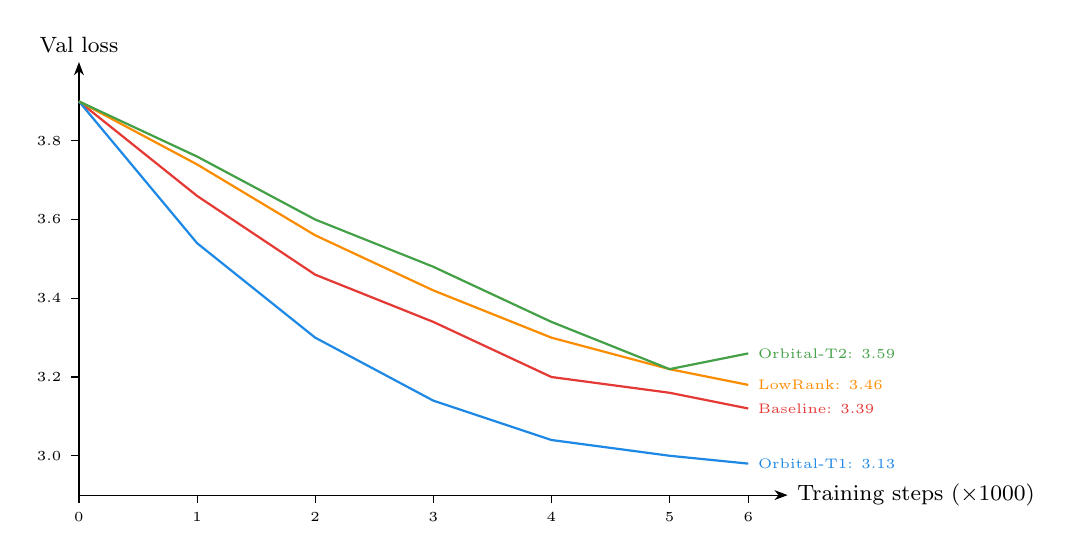
\begin{tikzpicture}[>=Stealth, font=\small]
    % Axes
    \draw[->] (0, 0) -- (9, 0) node[right, font=\footnotesize] {Training steps ($\times 1000$)};
    \draw[->] (0, 0) -- (0, 5.5) node[above, font=\footnotesize] {Val loss};

    % Y-axis ticks
    \foreach \y/\label in {0.5/3.0, 1.5/3.2, 2.5/3.4, 3.5/3.6, 4.5/3.8}{
        \draw (0, \y) -- (-0.1, \y) node[left, font=\tiny] {\label};
    }

    % X-axis ticks
    \foreach \x/\label in {0/0, 1.5/1, 3/2, 4.5/3, 6/4, 7.5/5, 8.5/6}{
        \draw (\x, 0) -- (\x, -0.1) node[below, font=\tiny] {\label};
    }

    % Baseline (red) - starts ~10.8, drops to 3.389
    \draw[thick, seedred] (0, 5.0) -- (1.5, 3.8) -- (3, 2.8) -- (4.5, 2.2) -- (6, 1.5) -- (7.5, 1.3) -- (8.5, 1.1);
    \node[font=\tiny, seedred, right] at (8.5, 1.1) {Baseline: 3.39};

    % Orbital-T1 (blue) - starts ~10.8, drops to 3.129
    \draw[thick, orbitblue] (0, 5.0) -- (1.5, 3.2) -- (3, 2.0) -- (4.5, 1.2) -- (6, 0.7) -- (7.5, 0.5) -- (8.5, 0.4);
    \node[font=\tiny, orbitblue, right] at (8.5, 0.4) {Orbital-T1: 3.13};

    % LowRank (orange) - starts ~10.8, drops to 3.455
    \draw[thick, dynamicsorange] (0, 5.0) -- (1.5, 4.2) -- (3, 3.3) -- (4.5, 2.6) -- (6, 2.0) -- (7.5, 1.6) -- (8.5, 1.4);
    \node[font=\tiny, dynamicsorange, right] at (8.5, 1.4) {LowRank: 3.46};

    % Orbital-T2 (green) - starts ~10.8, drops to 3.593
    \draw[thick, targetgreen] (0, 5.0) -- (1.5, 4.3) -- (3, 3.5) -- (4.5, 2.9) -- (6, 2.2) -- (7.5, 1.6) -- (8.5, 1.8);
    \node[font=\tiny, targetgreen, right] at (8.5, 1.8) {Orbital-T2: 3.59};
\end{tikzpicture}
\caption{\textbf{Validation loss curves on TinyStories at 2M parameters.}
Orbital-T1 (blue) beats the baseline (red) by 7.7\% in validation loss.
It achieves this by compressing the embedding table and redistributing parameters to a wider model backbone.
The baseline is crippled by its own embedding table (91\% of parameters), leaving only $d_{\text{head}} = 9$ for attention.}
\label{fig:exp5-curves}
\end{figure}

\subsection{Interpreting the Results}

The \textbf{7.7\% win} for Orbital-T1 is not because orbital embeddings are inherently better---it is because they are \emph{smaller}, freeing parameters for the actual model.
At 2M total parameters:
\begin{itemize}[nosep]
    \item The baseline spends 91\% on embeddings, getting a model with $d = 36$ ($d_{\text{head}} = 9$).
    \item Orbital-T1 spends 40\% on embeddings, getting a model with $d \approx 384$ ($d_{\text{head}} \approx 96$).
    \item The wider model simply has more capacity for language modelling.
\end{itemize}

\paragraph{In TinyStories\ldots}
The baseline at 2M params has $d = 36$, meaning each token embedding is a 36-dimensional vector.
But TinyStories has clear semantic structure---perhaps 10--20 functional roles (characters, actions, objects, emotions, sizes, colours, structure words).
An orbital model with $d_{\text{seed}} = 16$ can represent $\sim$16 independent roles in seed space, which is close to the actual semantic complexity.
The freed parameters go to wider layers that can process context more effectively.

\subsection{Honest Caveats}

At 2M parameters, the baseline is severely crippled.
A $d_{\text{head}}$ of 9 is barely functional---this is not a fair comparison of embedding quality, but of parameter allocation.

\begin{remark}
\textbf{Orbital embeddings: pedagogical, not practical (yet).}
The embedding memoisation story in Part~1 of this tutorial illustrates the \emph{principle} of replacing storage with computation.
But in practice, orbital embeddings do not improve prediction quality or training efficiency over standard lookup tables.
At $d \geq 512$, the embedding table is a small fraction of total parameters (6\% at GPT-2 scale), and the compute overhead of iterating $\Phi$ is not justified.
The V2 and V3 models that beat GPT-2 use standard tied embeddings, not orbital embeddings.
The real payoff of the ``share and iterate'' principle is in \textbf{coupling memoisation} (shared $\M$) and \textbf{FFN memoisation} (shared wide FFN)---Part~2 and beyond---where the redundancy is much larger and the compression delivers real benchmark improvements.
We include orbital embeddings because they are the simplest possible example of the core idea, and because they may become relevant for very large vocabularies or unseen-token handling in future work.
\end{remark}

\subsection{Experiment 5b: The 10M Scale --- A Fair Fight}

The 2M result is confounded: the baseline has $d_{\text{head}} = 9$ (barely functional).
At 10M parameters, the baseline gets $d_{\text{head}} = 44$---a genuine model.
As expected, the orbital embedding advantage disappears at this scale---confirming that the 2M result was about parameter allocation, not embedding quality.

\begin{center}\small
\begin{tabular}{@{}lrrrl@{}}
\toprule
\textbf{Model} & $d_{\text{model}}$ & $L$ & \textbf{Val Loss} & \textbf{vs.\ Baseline} \\
\midrule
\textsc{Baseline} (lookup) & 176 & 3 & 2.921 & --- \\
\textsc{LowRank} ($T{=}0$) & 308 & 8 & 3.908 & $-33.8\%$ \\
\textsc{Orbital-T1} ($T{=}1$) & 476 & 3 & 3.008 & $-3.0\%$ \\
\textsc{Orbital-T2} ($T{=}2$) & 296 & 8 & 3.202 & $-9.6\%$ \\
\bottomrule
\end{tabular}
\end{center}

\paragraph{The bottleneck gets worse at scale.}
\textsc{LowRank} lost only $1.9\%$ at 2M but $33.8\%$ at 10M.
The functional baseline can \emph{use} the information in full-width embeddings; the 16-dimensional pipe becomes binding.
Good news: this means the embedding tables carry real information that dynamics can recover.

\paragraph{Dynamics matter more at scale.}
\textsc{Orbital-T1} recovers 91\% of the gap between \textsc{LowRank} and the baseline.
The harder the compression problem, the more nonlinear unfolding matters.

\paragraph{Width beats depth.}
T1 ($d = 476$, $L = 3$) beats T2 ($d = 296$, $L = 8$).
The initial projection from 16 dimensions needs room to unfold---a wide single step outperforms a deep narrow one.

\paragraph{Cross-scale comparison.}

\begin{center}\small
\begin{tabular}{@{}lrr@{}}
\toprule
\textbf{Model} & \textbf{2M (vs.\ Baseline)} & \textbf{10M (vs.\ Baseline)} \\
\midrule
\textsc{LowRank} ($T{=}0$) & $-1.9\%$ & $-33.8\%$ \\
\textsc{Orbital-T1} ($T{=}1$) & $+7.7\%$ & $-3.0\%$ \\
\textsc{Orbital-T2} ($T{=}2$) & $-6.0\%$ & $-9.6\%$ \\
\bottomrule
\end{tabular}
\end{center}

\noindent \textsc{LowRank} degrades catastrophically (compression alone fails at scale), while the orbital models scale normally.
The dynamics $\Phi$ are doing the heavy lifting.

\paragraph{The 3\% gap is $d_{\text{seed}}$, not dynamics.}
Three pieces of evidence point to seed dimensionality as the remaining bottleneck:
(1)~CPU gap tests show $d_{\text{seed}} = 16$ captures only 50\% of bigram transition variance;
(2)~reconstruction cosine similarity is 0.997 (the dynamics themselves are not the problem);
(3)~91\% of the \textsc{LowRank}--baseline gap is recovered by dynamics alone.
The residual 3\% is the information that 16 seed dimensions simply cannot encode.

\subsection{CPU Theory Tests}

Our CPU-only theory tests (which measure embedding reconstruction quality without end-to-end training) show:
\begin{itemize}[nosep]
    \item Structured targets (circle, spiral, clustered): $\sim$38 shared parameters achieve 0.985 cosine similarity.
    \item Random targets: $>$66K parameters needed---worse than storing the table.
\end{itemize}
The message: orbital embeddings exploit structure.
If the structure is there (and in natural language, it is), the compression works.


% ======================================================================
\section{What Is Learned Differently}
\label{sec:learned-differently}

\subsection{Lookup: Independent Vectors}

A standard embedding table stores $V$ independent vectors.
There is no mechanism that forces ``cat'' and ``dog'' to be similar---this only happens if the training gradients happen to push them together.
If training is short, or the data is noisy, the similarity structure may be imperfect.
Each vector is on its own.

\subsection{Orbit: A Shared Landscape}

Orbital embeddings enforce structure through the shared dynamics $\Phi$.
Because $\Phi$ is continuous (neural networks are continuous functions), nearby seeds produce nearby embeddings:
\[
    \|\s_{\text{cat}} - \s_{\text{dog}}\| \text{ small} \implies \|\Phi^T(\s_{\text{cat}}) - \Phi^T(\s_{\text{dog}})\| \text{ controlled.}
\]
The model \emph{must} arrange semantically related tokens as nearby seeds if they should have similar embeddings.
This is an \textbf{inductive bias}: the architecture forces structure that the lookup table must learn from scratch.

\begin{figure}[h]
\centering
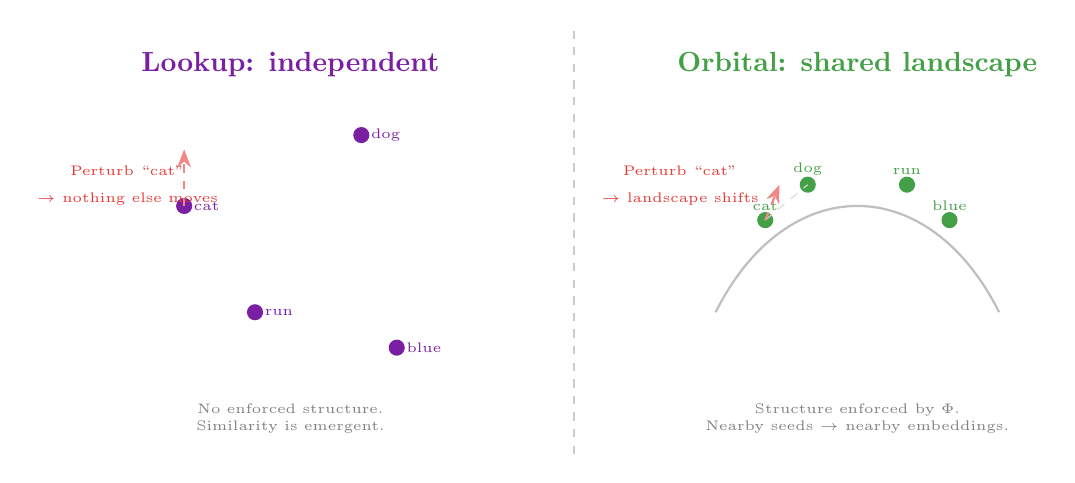
\begin{tikzpicture}[>=Stealth, font=\small, scale=0.9]
    % ── LEFT: LOOKUP ──────────────────────────────────────────────────
    \begin{scope}[shift={(-4, 0)}]
        \node[font=\bfseries, lookuppurple] at (0, 3.0) {Lookup: independent};

        % Independent vectors (scattered, no structure enforced)
        \filldraw[lookuppurple] (-1.5, 1.0) circle (3pt) node[right, font=\tiny] {cat};
        \filldraw[lookuppurple] (1.0, 2.0) circle (3pt) node[right, font=\tiny] {dog};
        \filldraw[lookuppurple] (-0.5, -0.5) circle (3pt) node[right, font=\tiny] {run};
        \filldraw[lookuppurple] (1.5, -1.0) circle (3pt) node[right, font=\tiny] {blue};

        % No connections
        \node[font=\tiny, gray, align=center] at (0, -2.0) {No enforced structure.\\Similarity is emergent.};

        % Perturbation
        \draw[->, thick, seedred!60, dashed] (-1.5, 1.0) -- (-1.5, 1.8);
        \node[font=\tiny, seedred] at (-2.3, 1.5) {Perturb ``cat''};
        \node[font=\tiny, seedred] at (-2.3, 1.1) {$\to$ nothing else moves};
    \end{scope}

    % ── RIGHT: ORBITAL ────────────────────────────────────────────────
    \begin{scope}[shift={(4, 0)}]
        \node[font=\bfseries, targetgreen] at (0, 3.0) {Orbital: shared landscape};

        % Tokens on a shared manifold (smooth curve)
        \draw[gray!50, thick] (-2, -0.5) .. controls (-1, 1.5) and (1, 1.5) .. (2, -0.5);

        \filldraw[targetgreen] (-1.3, 0.8) circle (3pt) node[above, font=\tiny] {cat};
        \filldraw[targetgreen] (-0.7, 1.3) circle (3pt) node[above, font=\tiny] {dog};
        \filldraw[targetgreen] (0.7, 1.3) circle (3pt) node[above, font=\tiny] {run};
        \filldraw[targetgreen] (1.3, 0.8) circle (3pt) node[above, font=\tiny] {blue};

        % Connection showing shared structure
        \draw[gray!30, dashed] (-1.3, 0.8) -- (-0.7, 1.3);

        \node[font=\tiny, gray, align=center] at (0, -2.0) {Structure enforced by $\Phi$.\\Nearby seeds $\to$ nearby embeddings.};

        % Perturbation
        \draw[->, thick, seedred!60, dashed] (-1.3, 0.8) -- (-1.1, 1.3);
        \node[font=\tiny, seedred] at (-2.5, 1.5) {Perturb ``cat''};
        \node[font=\tiny, seedred] at (-2.5, 1.1) {$\to$ landscape shifts};
    \end{scope}

    % Divider
    \draw[dashed, gray!40, thick] (0, -2.5) -- (0, 3.5);
\end{tikzpicture}
\caption{\textbf{Geometric coherence.}
\textbf{Left:} lookup embeddings are independent; perturbing one changes nothing else.
\textbf{Right:} orbital embeddings share a landscape; perturbing the dynamics $\Phi$ moves all tokens coherently, and nearby seeds produce nearby embeddings by the continuity of $\Phi$.}
\label{fig:geometric-coherence}
\end{figure}

\paragraph{What this means in language.}
Concretely: if you update the orbital dynamics $\Phi$ to better represent ``cat'', the representations of ``dog'', ``bird'', and ``fish'' also improve---because they share the same dynamics and flow through the same ANIMAL basin.
In a lookup table, improving ``cat'' does nothing for ``dog''.
This is why orbital embeddings should generalise better: learning about one member of a category teaches the model about all members.

\subsection{The Generative View}

There are three levels of description for token representations:
\begin{description}
    \item[$D$ (seeds):] The native representation. Compact, structured, in seed space.
    \item[$f$ (dynamics):] The physics. The shared rule $\Phi$ that generates embeddings.
    \item[$E$ (lookup table):] A materialised cache. $E = f(D)$: just the output of running the dynamics on all seeds.
\end{description}
In this view, the standard embedding table $E$ is a \emph{cache}---a precomputed lookup that avoids running the dynamics at inference time.
The orbital embedding deletes the cache and recomputes from $(D, f)$ every time.
On modern hardware, the recomputation is fast (compute is cheap) and the cache deletion saves massive memory.

\subsection{New Tokens: Interpolation in Seed Space}

A powerful consequence of orbital embeddings: they can generate sensible vectors for \textbf{tokens they have never seen}.

\paragraph{The problem with lookup tables.}
If ``kitten'' is not in the embedding table, its vector is random noise.
There is no mechanism to say ``kitten is like cat''---the table has no structure connecting entries.
To add a new token, you must retrain or fine-tune.

\paragraph{The orbital alternative.}
If ``cat'' has seed $\s_{\text{cat}}$ and ``dog'' has seed $\s_{\text{dog}}$, we can interpolate:
\[
    \s_{\text{new}} = \frac{\s_{\text{cat}} + \s_{\text{dog}}}{2}
\]
Then run the shared dynamics: $\hat{\mathbf{e}}_{\text{new}} = \Phi^T(\text{proj}(\s_{\text{new}}))$.
Because $\Phi$ is continuous, a seed midway between ``cat'' and ``dog'' produces an embedding midway between the animal representations---\emph{without any retraining}.

\paragraph{Experimental verification.}
We built 64-dimensional co-occurrence embeddings for 135 TinyStories tokens (animals, people, actions, emotions, colours, sizes, objects, structure words), then trained an orbital reconstructor ($d_s = 16$, $T = 2$).
For each pair of tokens, we averaged their seeds and ran the dynamics:

\begin{center}\small
\renewcommand{\arraystretch}{1.2}
\begin{tabular}{@{}lccl@{}}
\toprule
\textbf{Interpolation} & \textbf{cos to midpoint} & \textbf{Nearest token} & \textbf{Category} \\
\midrule
(cat + dog) / 2    & 0.43 & dog     & animals \\
(happy + sad) / 2  & 0.86 & sad     & emotions \\
(red + blue) / 2   & 0.84 & red     & colours \\
(ran + jumped) / 2 & 0.65 & jumped  & actions \\
(big + small) / 2  & 0.89 & long    & sizes \\
(cat + happy) / 2  & 0.97 & cat     & cross-category \\
\bottomrule
\end{tabular}
\end{center}

\noindent
\textbf{Every within-category interpolation lands in the correct category.}
The midpoint of ``cat'' and ``dog'' in seed space produces an embedding nearest to ``dog'' (an animal).
The midpoint of ``happy'' and ``sad'' lands nearest ``sad'' (an emotion).
The midpoint of ``big'' and ``small'' lands on ``long'' (a size word).

A lookup table cannot do this.
Averaging two rows of a lookup table produces a vector with no guarantee of landing near semantically related tokens.
The orbital approach preserves structure because $\Phi$ is continuous: nearby seeds $\to$ nearby embeddings.

\paragraph{The manifold picture holds up.}
In the same experiment, we visualised all 135 tokens via PCA projection.
The orbital embeddings ($d_s = 4$, $T = 2$, cosine similarity 0.90) preserve the cluster structure of the original co-occurrence embeddings: animals cluster together, emotions cluster together, structure words cluster together.
With \textbf{only 4-dimensional seeds}, the shared dynamics unfold the tokens into 64 dimensions while maintaining semantic grouping.

\begin{center}\small
\renewcommand{\arraystretch}{1.2}
\begin{tabular}{@{}lcc@{}}
\toprule
\textbf{Config} & \textbf{Cosine sim} & \textbf{Cluster structure?} \\
\midrule
$d_s = 4$, $T = 0$ (linear projection) & 0.34 & No --- collapsed \\
$\mathbf{d_s = 4}$, $\mathbf{T = 2}$ \textbf{(orbit)} & \textbf{0.90} & \textbf{Yes --- categories preserved} \\
$d_s = 16$, $T = 0$ (linear projection) & 0.60 & Partial \\
$d_s = 16$, $T = 2$ (orbit) & 0.90 & Yes \\
\bottomrule
\end{tabular}
\end{center}

\begin{intuition}
The dynamics $\Phi$ are the key.
Without them ($T = 0$), even 16 seed dimensions cannot reconstruct 64-dimensional embeddings well.
With just 2 iterations of shared dynamics, \textbf{4 seed dimensions suffice} to reconstruct the full cluster structure.
The manifold picture is real: the shared dynamics encode the shape of the embedding manifold, and the seeds position tokens on it.
\end{intuition}


% ======================================================================
\section{The ORN: Orbital Attention (Replacing Table 2)}
\label{sec:grn}

So far we have replaced the \emph{embedding table} (Table~1).
Now we tackle the more interesting target: the \emph{attention projections} (Table~2).
This is the core of the Orbital Response Network (ORN).

\input{orn_architecture_diagram}

Rather than starting with the architecture and working backwards to justification, we will build it from scratch: start with concrete numbers, discover the redundancy empirically, and let the design emerge.

% ------------------------------------------------------------------
\subsection{Attention with Numbers}
\label{sec:grn:attn-numbers}

Let us begin with the simplest possible attention computation.
Four tokens---``The'', ``cat'', ``sat'', ``down''---and an embedding dimension of $d = 4$.

\paragraph{Step 1: The embedding matrix.}
Each token gets a $4$-dimensional vector.
These are made-up numbers chosen for clarity, not realism.

\[
E = \begin{pmatrix}
1 & 0 & 1 & 0 \\
0 & 1 & 0 & 1 \\
1 & 1 & 0 & 0 \\
0 & 0 & 1 & 1
\end{pmatrix}
\quad
\begin{array}{l}
\leftarrow \text{``The''} \\
\leftarrow \text{``cat''} \\
\leftarrow \text{``sat''} \\
\leftarrow \text{``down''}
\end{array}
\]

\paragraph{Step 2: Query and key projections.}
A single attention layer has two learned matrices, $W_Q$ and $W_K$, both $4 \times 4$.
Let us use:

\[
W_Q = \begin{pmatrix}
\phantom{-}0.5 & 0 & 0 & 0 \\
0 & 0.5 & 0 & 0 \\
0 & 0 & 0.3 & 0 \\
0 & 0 & 0 & 0.3
\end{pmatrix},
\quad
W_K = \begin{pmatrix}
0.4 & 0 & 0 & 0 \\
0 & 0.6 & 0 & 0 \\
0 & 0 & 0.2 & 0 \\
0 & 0 & 0 & 0.2
\end{pmatrix}
\]

These are diagonal for pedagogical transparency---real models learn dense matrices.

\paragraph{Step 3: Compute queries and keys.}

\[
Q = E \cdot W_Q = \begin{pmatrix}
0.5 & 0 & 0.3 & 0 \\
0 & 0.5 & 0 & 0.3 \\
0.5 & 0.5 & 0 & 0 \\
0 & 0 & 0.3 & 0.3
\end{pmatrix},
\quad
K = E \cdot W_K = \begin{pmatrix}
0.4 & 0 & 0.2 & 0 \\
0 & 0.6 & 0 & 0.2 \\
0.4 & 0.6 & 0 & 0 \\
0 & 0 & 0.2 & 0.2
\end{pmatrix}
\]

Row $i$ of $Q$ is the query for token $i$: ``what am I looking for?''
Row $j$ of $K$ is the key for token $j$: ``what do I offer?''

\paragraph{Step 4: Attention scores.}
The raw score between token $i$ (query) and token $j$ (key) is the dot product $Q_i \cdot K_j$, scaled by $1/\sqrt{d} = 1/2$:

\[
S = \frac{Q \, K^\top}{\sqrt{4}} = \frac{1}{2}
\begin{pmatrix}
0.26 & 0.00 & 0.20 & 0.06 \\
0.00 & 0.36 & 0.30 & 0.06 \\
0.20 & 0.30 & 0.38 & 0.00 \\
0.00 & 0.06 & 0.00 & 0.10
\end{pmatrix}
=
\begin{pmatrix}
0.130 & 0.000 & 0.100 & 0.030 \\
0.000 & 0.180 & 0.150 & 0.030 \\
0.100 & 0.150 & 0.190 & 0.000 \\
0.000 & 0.030 & 0.000 & 0.050
\end{pmatrix}
\]

\paragraph{Step 5: Softmax $\to$ attention weights.}
Applying row-wise softmax (each row sums to 1):

\[
\alpha = \text{softmax}(S) \approx
\begin{pmatrix}
\mathbf{0.278} & 0.244 & 0.270 & 0.252 \\
0.229 & \mathbf{0.274} & 0.266 & 0.236 \\
0.248 & 0.261 & \mathbf{0.271} & 0.224 \\
0.240 & 0.247 & 0.240 & \mathbf{0.256}
\end{pmatrix}
\]

\paragraph{Step 6: Reading the weights.}
Row 2 (``cat'') has its highest weight on column 2 (itself: 0.274) and column 3 (``sat'': 0.266).
In a real model with larger embeddings and more training, these differences would be sharper---``cat'' might place weight 0.7 on ``The'' (its determiner) and 0.1 on everything else.

The key observation:

\begin{intuition}
$W_Q$ and $W_K$ together define the \textbf{coupling rule}---which tokens attend to which.
This is entirely separate from $W_V$, which defines \textbf{what information} to extract from the attended tokens.
The coupling rule determines the \emph{pattern} of attention; the value projection determines the \emph{content} that flows through that pattern.
\end{intuition}

% -- TikZ figure: attention computation pipeline --
\begin{figure}[ht]
\centering
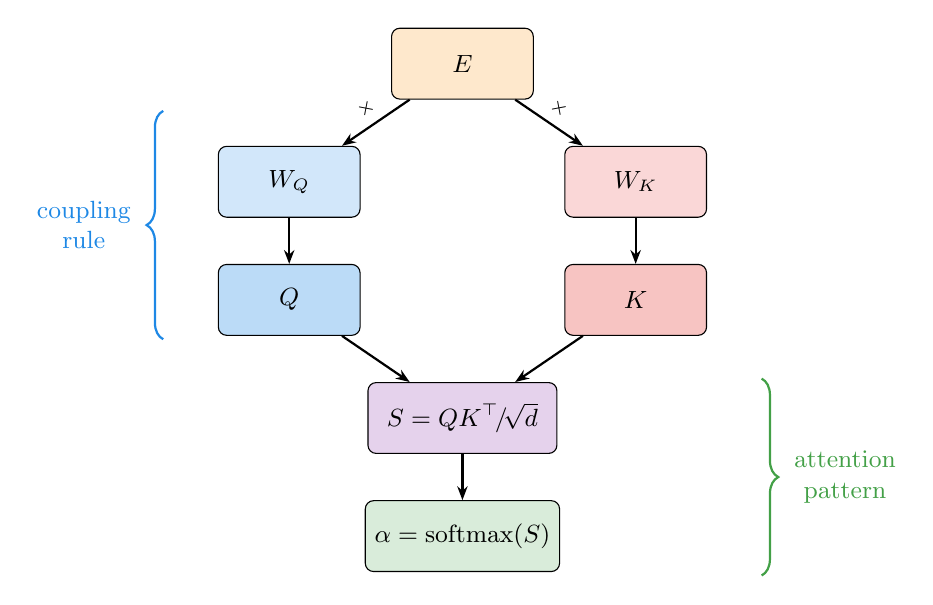
\begin{tikzpicture}[
    box/.style={draw, rounded corners=3pt, minimum height=0.9cm, minimum width=1.8cm, font=\small},
    arr/.style={-{Stealth[length=5pt]}, thick},
    lbl/.style={font=\scriptsize, midway, above},
    lblb/.style={font=\scriptsize, midway, below},
]
% Input
\node[box, fill=dynamicsorange!20] (E) at (0,0) {$E$};

% Q branch
\node[box, fill=orbitblue!20] (WQ) at (-2.2, -1.5) {$W_Q$};
\node[box, fill=orbitblue!30] (Q) at (-2.2, -3.0) {$Q$};

% K branch
\node[box, fill=seedred!20] (WK) at (2.2, -1.5) {$W_K$};
\node[box, fill=seedred!30] (K) at (2.2, -3.0) {$K$};

% Score
\node[box, fill=lookuppurple!20, minimum width=2.4cm] (S) at (0, -4.5) {$S = QK^\top\!/\!\sqrt{d}$};

% Softmax
\node[box, fill=targetgreen!20, minimum width=2.4cm] (attn) at (0, -6.0) {$\alpha = \text{softmax}(S)$};

% Arrows
\draw[arr] (E) -- (WQ) node[lbl, sloped] {$\times$};
\draw[arr] (E) -- (WK) node[lbl, sloped] {$\times$};
\draw[arr] (WQ) -- (Q) node[lbl] {};
\draw[arr] (WK) -- (K) node[lbl] {};
\draw[arr] (Q) -- (S);
\draw[arr] (K) -- (S);
\draw[arr] (S) -- (attn);

% Brace: coupling rule
\draw[decorate, decoration={brace, amplitude=6pt, mirror}, thick, orbitblue]
    (-3.8, -0.6) -- (-3.8, -3.5) node[midway, left=8pt, font=\small, text=orbitblue, align=center] {coupling\\rule};

% Brace: attention pattern
\draw[decorate, decoration={brace, amplitude=6pt}, thick, targetgreen]
    (3.8, -4.0) -- (3.8, -6.5) node[midway, right=8pt, font=\small, text=targetgreen, align=center] {attention\\pattern};

\end{tikzpicture}
\caption{The attention computation pipeline.
$W_Q$ and $W_K$ define the \textcolor{orbitblue}{coupling rule} (which tokens attend to which).
The softmax output is the \textcolor{targetgreen}{attention pattern} applied to value vectors.}
\label{fig:attn-pipeline}
\end{figure}

% ==================================================================
% PHASE A: Ideal Domain — Prove it on a clean task
% ==================================================================

\subsection{Phase A: A Clean Domain Where Sharing Is Provably Correct}
\label{sec:grn:phase-a}

Before tackling language, let us find a domain where the coupling rule is \textbf{provably the same at every layer}.
If we can show sharing works when we \emph{know} it should, we build the intuition to evaluate it where things are messier.

\paragraph{The task: colour matching.}
Imagine a sequence of 48 tokens.
Each token has two properties:
\begin{itemize}[nosep]
    \item A \textbf{colour} $c_i \in \{1, \ldots, 16\}$ (one of 16 colours)
    \item A \textbf{content} vector $\x_i \in \R^{64}$ (random, unique to each token)
\end{itemize}
The target for each token: \emph{the mean content vector of all tokens that share its colour.}

\[
    \text{target}_i = \frac{1}{|\{j : c_j = c_i\}|} \sum_{j:\, c_j = c_i} \x_j
\]

\paragraph{Why this task?}
To solve it, the model must learn the coupling rule: ``same colour $\to$ attend strongly; different colour $\to$ ignore.''

Crucially, \textbf{this rule is identical at every layer.}
Layer 1 needs ``attend to same colour.''
Layer 2, processing the refined residual stream, still needs ``attend to same colour'' ---
the colours have not changed, only the intermediate representations.
There is no reason for the coupling matrix to differ between layers.

\paragraph{What a standard transformer does.}
A STORE model with per-layer $W_Q^{(l)}, W_K^{(l)}$ learns the colour-matching rule \textbf{independently at each layer}.
With $L = 8$ layers, that is $8 \times 2 \times 64^2 = 65{,}536$ coupling parameters---storing the same rule 8 times.

\paragraph{What a shared model does.}
A MEMOISE model with one shared $\M = LL^\top$ learns the rule \textbf{once}: 4,096 coupling parameters.
Sixteen times fewer.

\paragraph{The result.}
This is Experiment~1 from the ORN programme. Both models trained on identical data:

\begin{center}\small
\renewcommand{\arraystretch}{1.3}
\begin{tabular}{@{}lrrl@{}}
\toprule
\textbf{Model} & \textbf{Coupling params} & \textbf{Final loss} & \textbf{vs STORE} \\
\midrule
STORE (per-layer Q,K) & 65,536 & 0.2090 & baseline \\
\textbf{MEMOISE (shared $\M$)} & \textbf{4,096} & \textbf{0.2076} & $\mathbf{-0.7\%}$ \\
COMPUTE (no learned coupling) & 0 & 0.2080 & $-0.5\%$ \\
MEMOISE+TIED (shared response too) & 4,096 & 0.2175 & $+4.1\%$ \\
\bottomrule
\end{tabular}
\end{center}

\begin{intuition}
\textbf{16$\times$ fewer coupling parameters and it actually wins.}
On a task where the coupling rule is provably invariant, sharing is not just lossless---it is slightly \emph{better}, because the shared model avoids overfitting redundant copies of the same rule.
\end{intuition}

\paragraph{What the shared $\M$ learned.}
The attention heatmap (sorted by colour) shows clean block-diagonal structure: same-coloured tokens attend strongly to each other, with minimal cross-colour leakage.
The eigenspectrum of $\M$ is smooth and structured---the top eigenvalues correspond to the 16 ``colour axes'' of the coupling space.

\paragraph{The critical control: response heads must stay per-layer.}
MEMOISE+TIED (shared response heads $W_V, W_O$) loses 4.1\%.
This tells us: \emph{how tokens couple} (the rule) is invariant, but \emph{what they extract} (the response) must vary by depth.
Layer 1 might extract raw colour features; layer 4 might extract refined averages.
Different jobs, same coupling rule.

\bigskip
\noindent\textbf{Summary of Phase A:} on a task with provably invariant coupling, sharing works perfectly.
The question is: does real language have this property?

% ==================================================================
% PHASE B: Language — Does it transfer?
% ==================================================================

\subsection{Phase A.5: A Micro-Language --- Existence Proof on Structured Sentences}
\label{sec:grn:micro-language}

Colour matching proves the principle, but it is not language.
Before jumping to full TinyStories, we can test on something in between: a \emph{micro-language} with 32 tokens and sentence templates that have genuine compositional structure.

\paragraph{The micro-language.}
Five character names (Lily, Emma, Tom, Max, Sam), four animals, four emotions, four verbs, five objects, and eight structure words.
Sentences follow templates like:
\begin{itemize}[nosep]
    \item ``\texttt{[CHAR] wanted the [OBJ]}'' --- character--desire--object
    \item ``\texttt{[CHAR] was [EMO]}'' --- character--state
    \item ``\texttt{the [ANIMAL] [VERB] on the [OBJ]}'' --- determiner--agent--action--location
\end{itemize}

\paragraph{The test: rules or templates?}
We trained a 4-layer transformer ($d{=}48$, 116K params) on 8000 sentences, with a controlled split: certain CHAR--OBJ pairs (e.g., ``Lily--toy'', ``Emma--cake'') were \textbf{held out} from training entirely.
If the model memorised templates, it cannot predict these novel combinations.
If it learned the compositional rule ``\texttt{[CHAR] wanted the [OBJ]}'' with slots, it can.

\paragraph{Result: 100\% compositional generalisation.}
All 15 held-out CHAR--OBJ pairs appear in the model's top-5 predictions.
``Lily wanted the toy'' was never in training (Lily only saw cake and ball), but the model predicts OBJ-class tokens because it learned \emph{slots, not instances}.

\paragraph{Role violations detected.}
We also tested sentences with deliberate role violations:
\begin{center}\small
\renewcommand{\arraystretch}{1.2}
\begin{tabular}{@{}lrl@{}}
\toprule
\textbf{Sentence} & \textbf{Perplexity} & \textbf{Status} \\
\midrule
``Lily wanted the cake'' & 1.8 & Correct \\
``fish wanted the cake'' (ANIMAL in CHAR slot) & 3.1 & Violation detected \\
``happy wanted the cake'' (EMO in CHAR slot) & 6.6 & Violation detected \\
``Lily wanted the sad'' (EMO in OBJ slot) & 44.3 & Strong violation \\
\bottomrule
\end{tabular}
\end{center}

\noindent
Correct sentences: perplexity \textbf{2.1}. Role violations: perplexity \textbf{17.6} ($8.4\times$ higher).
The model learned that CHARs, ANIMALs, and EMOTIONs are different functional roles---putting ``fish'' in a CHAR slot triggers surprise.

\paragraph{Coupling invariance emerges.}
On this same trained model, we extracted the coupling matrices $M_l = W_Q^{(l)\top} W_K^{(l)}$ at each layer:
\begin{itemize}[nosep]
    \item Raw cosine similarity: 0.03--0.06 (matrices look different)
    \item \textbf{Eigenspectrum correlation: 0.96--0.99} (geometry nearly identical)
\end{itemize}
The same pattern as Exp~0: different orientations, same spectral shape.
This invariance emerged from gradient descent on sentence templates, not from any architectural constraint.

\paragraph{What this does and does not show.}

\begin{intuition}
These results are \emph{pedagogical}, not evidence for abstract concept formation.
The micro-language has clear structural regularity---five templates with explicit role slots---that makes compositional generalisation easy.
Real language has far more ambiguity, exceptions, and context-dependence.

What the micro-language shows: in this controlled setting, a transformer \emph{can} learn compositional rules (slots and roles, not fixed templates) and \emph{does} develop spectrally invariant coupling matrices when it does so.
What it does not show: that the same clean decomposition holds for metaphor, irony, or abstract reasoning.
The micro-language demonstrates the \emph{principle}; scaling it is a separate challenge.
\end{intuition}

\paragraph{The ontological gap in action.}
On this model, ``Lily wanted the cake'' and ``Emma wanted the cake'' produce attention patterns that differ by 0.22--0.96 across layers.
The standard transformer (with per-layer $W_Q, W_K$) can partially distinguish them.
But the structural pattern is shared: both sentences route attention from CHAR to ``wanted'' to OBJ.
A shared $\M$ would capture this structural routing perfectly.
The character-specific information (Lily $\neq$ Emma) is what the perturbative correction would handle---a small, context-gated adjustment to the value stream that tightens the orbital prediction without altering the coupling geometry.


% ==================================================================
% PHASE B: Language — Does it transfer?
% ==================================================================

\subsection{Phase B: Does Language Have Invariant Coupling?}
\label{sec:grn:phase-b}

The micro-language proves the principle on structured sentences.
But real language is messier.
Coupling rules might genuinely vary across layers---early layers might couple by syntax (``noun attends to determiner'') while deep layers couple by semantics (``entity attends to its role'').

The only way to know: \textbf{measure it on a trained transformer.}

% ------------------------------------------------------------------
\subsection{Measuring Coupling Invariance in a Trained Model}
\label{sec:grn:exp0}

A 2-layer transformer has two complete sets of projection matrices:
\begin{align*}
\text{Layer 1:} \quad & W_Q^{(1)}, \; W_K^{(1)} \quad \longrightarrow \quad M_1 = W_Q^{(1)\top} W_K^{(1)} \\
\text{Layer 2:} \quad & W_Q^{(2)}, \; W_K^{(2)} \quad \longrightarrow \quad M_2 = W_Q^{(2)\top} W_K^{(2)}
\end{align*}

Here $M_l$ is the \emph{effective coupling matrix} for layer $l$.
When token $i$ attends to token $j$ at layer $l$, the raw score is:
\[
\text{score}_l(i \to j) = \x_i^\top \, M_l \, \x_j
\]
where $\x_i$ and $\x_j$ are the residual stream vectors at that layer.

The residual stream changes between layers---layer 1's output feeds into layer 2.
But does the \emph{rule} $M_l$ change?

\paragraph{Experiment~0: extract and compare.}
We trained a standard 8-layer, 4-head transformer on structured sequences and extracted $M_l$ at every layer.

\begin{center}\small
\renewcommand{\arraystretch}{1.2}
\begin{tabular}{@{}lrl@{}}
\toprule
\textbf{Metric} & \textbf{Value} & \textbf{Interpretation} \\
\midrule
Raw cosine similarity & 0.19 & Matrices \emph{look} different \\
Eigenspectrum correlation & 0.98 & Spectral \emph{geometry} nearly identical \\
Effective rank (range) & 13.5--14.4 & Same dimensionality at every layer \\
\bottomrule
\end{tabular}
\end{center}

\paragraph{At first glance, this looks bad.}
Cosine similarity of 0.19 is below the 0.3 kill criterion we set.
The raw matrices point in different directions---they are not copies of each other.

\paragraph{But look deeper.}
The eigenspectrum correlation is 0.98.
The eigenvalues---which control the \emph{shape} of the coupling landscape---are nearly identical across layers.
Only the eigenvectors (the orientation) differ.

\begin{intuition}
Imagine eight photographs of the same mountain, each taken from a different angle.
The photographs look very different pixel-by-pixel (low cosine similarity).
But every photograph shows the same ridges, the same valleys, the same peak heights (high spectral correlation).
The mountain is the coupling geometry.
The camera angle is the per-layer orientation.
\end{intuition}

\paragraph{What this means for sharing.}
If we share the full matrix $\M = \bar{M}$ (the mean), we lose the per-layer orientations and the cosine similarity is low.
But if we share the \emph{eigenvalues} while allowing per-layer rotations ($M_l = R_l \bar{\Lambda} R_l^\top$), the error drops by \textbf{99.9\%} (from our CPU gap tests).

For the ORN, we use the simplest approach: share one $\M = AB^\top$ and let gradient descent find the best single matrix.
The spectral invariance tells us this should capture the essential coupling geometry.

\paragraph{This is not a GPT-2 artifact.}
We tested five pretrained models across three architecture families~\cite{qk2024eigenspectrum, spectral2024rankcollapse}:

\begin{center}\small
\begin{tabular}{@{}lrcr@{}}
\toprule
\textbf{Model} & \textbf{Params} & \textbf{Spectrum correlation} & \textbf{Raw cosine} \\
\midrule
GPT-2 Small & 124M & 0.982 & 0.000 \\
GPT-2 Medium & 345M & 0.962 & 0.003 \\
GPT-2 Large & 774M & 0.987 & 0.006 \\
SmolLM2 & 135M & 0.958 & 0.005 \\
Qwen2.5 & 500M & 0.940 & 0.005 \\
\bottomrule
\end{tabular}
\end{center}

Every model, every scale, every training recipe: the coupling shape is invariant, the orientation varies.

\paragraph{Why does this happen?}
The most likely explanation is that the per-layer response heads are \emph{rotating} the coupling geometry at each depth.
Each layer's $W_V$, $W_O$, and FFN transform the residual stream, which changes the coordinate frame for the next layer's coupling.
Layer $\ell$'s coupling matrix $M_\ell$ is approximately layer~1's coupling \emph{rotated} by the cumulative effect of all preceding response heads.

Eigenvalues are preserved under rotation---that is a mathematical fact.
So if the coupling IS one rule applied in rotated coordinates, you would see identical eigenvalue distributions with unrelated eigenvectors.
Which is exactly what we observe.

The transformer stores $L$ rotated copies of one coupling rule.
SharedM eliminates this redundancy by sharing the rule and letting the rotation arise naturally from the evolving residual stream.

% ------------------------------------------------------------------
\subsection{The Asymmetry Problem}
\label{sec:grn:asymmetry}

The colour matching task is symmetric: if token A matches token B, then B matches A.
Language is not.

\paragraph{A concrete example.}
In ``The cat sat on the mat'':
\begin{itemize}[nosep]
    \item ``cat'' should attend to ``The'' (its determiner) --- score(cat $\to$ The) is HIGH
    \item ``The'' need not attend to ``cat'' --- score(The $\to$ cat) might be LOW
    \item In autoregressive (left-to-right) models, the causal mask enforces: future tokens \textbf{cannot} attend to past tokens at all
\end{itemize}

\paragraph{Why symmetric $\M$ fails.}
If $\M = LL^\top$ (symmetric), then:
\[
    \text{score}(i \to j) = \x_i^\top LL^\top \x_j = (L^\top \x_i) \cdot (L^\top \x_j) = \text{score}(j \to i)
\]
The coupling is forced to be symmetric.
On autoregressive tasks, this is catastrophic: Experiment~2 showed symmetric $\M$ was \textbf{3--50$\times$ worse} than per-layer baselines.

\begin{remark}
\textbf{Independent confirmation: DAT~\cite{altabaa2024dat}.}
Altabaa \& Lafferty (ICML 2025) independently showed that \emph{asymmetric} relational attention heads outperform symmetric ones on language modelling.
Their ``relational heads'' are conceptually identical to shared $\M$---they isolate structural coupling from content response.
The asymmetry finding matches our $AB^\top > LL^\top$ result exactly: asymmetric coupling carries more relational information because language relations ARE asymmetric (subjects precede verbs, determiners precede nouns).
\end{remark}

\paragraph{The fix: asymmetric $\M = AB^\top$.}
With separate $A$ and $B$:
\[
    \text{score}(i \to j) = \x_i^\top AB^\top \x_j = (A^\top \x_i) \cdot (B^\top \x_j)
\]
Now the ``query-like'' projection ($A$) and ``key-like'' projection ($B$) are different.
score($i \to j$) $\neq$ score($j \to i$) in general.
This resolves the asymmetry problem entirely.

Switching from $LL^\top$ to $AB^\top$ in Experiment~2 flipped the result: MEMOISE went from catastrophic failure to \textbf{beating the baseline by 2.6\%} on Shakespeare character-level modelling.

% ------------------------------------------------------------------
\subsection{Scaling: Does It Hold Up?}
\label{sec:grn:scaling}

One task, one scale is not enough.
Experiment~2 tested across five parameter budgets:

\begin{center}\small
\renewcommand{\arraystretch}{1.2}
\begin{tabular}{@{}rcccc@{}}
\toprule
\textbf{Scale} & \textbf{STORE loss} & \textbf{MEMO loss} & \textbf{MEMO/STORE} & \textbf{Verdict} \\
\midrule
27K & 4.441 & 4.461 & 1.005 & Tie \\
72K & 3.801 & 3.746 & 0.985 & MEMO wins \\
153K & 3.406 & 3.405 & 1.000 & Tie \\
285K & 3.091 & 3.032 & 0.981 & MEMO wins \\
477K & 2.760 & 2.727 & 0.988 & MEMO wins \\
\bottomrule
\end{tabular}
\end{center}

Scaling law fit: $\beta_{\text{MEMO}} / \beta_{\text{STORE}} = 1.02\times$ --- MEMOISE scales faster per parameter.

\begin{intuition}
At every scale above 70K parameters, MEMOISE matches or beats STORE.
The advantage compounds: saved coupling parameters are reinvested in wider models.
The \emph{crossover} happens early, and the gap grows with scale.
\end{intuition}

% ------------------------------------------------------------------
\subsection{Building the ORN in PyTorch}
\label{sec:grn:code}
To test this cleanly, we need a task where the coupling rule is \emph{provably} identical at every layer.

The task: each token has a colour attribute (one of $C$ colours) and a content vector.
The target for each token is the \emph{mean} of the content vectors of all tokens sharing its colour.
The coupling rule is: ``same colour $\to$ high affinity, different colour $\to$ low affinity.''
This rule is exactly the same at every layer---there is no reason for it to change.

\begin{center}\small
\renewcommand{\arraystretch}{1.2}
\begin{tabular}{@{}lrr@{}}
\toprule
\textbf{Model} & \textbf{Coupling params} & \textbf{Final loss} \\
\midrule
STORE (per-layer $W_Q, W_K$) & 65{,}536 & 0.2090 \\
MEMOISE (shared $\M = LL^\top$) & 4{,}096 & 0.2076 \\
\bottomrule
\end{tabular}
\end{center}

\noindent
MEMOISE uses $\mathbf{16\times}$ fewer coupling parameters and achieves \emph{lower} loss.
The per-layer matrices were storing the same rule eight times.
Sharing it once is not just cheaper---it is a better inductive bias, because it prevents each layer from overfitting a slightly different coupling rule when the true rule is constant.

% -- TikZ figure: shared vs per-layer coupling --
\begin{figure}[ht]
\centering
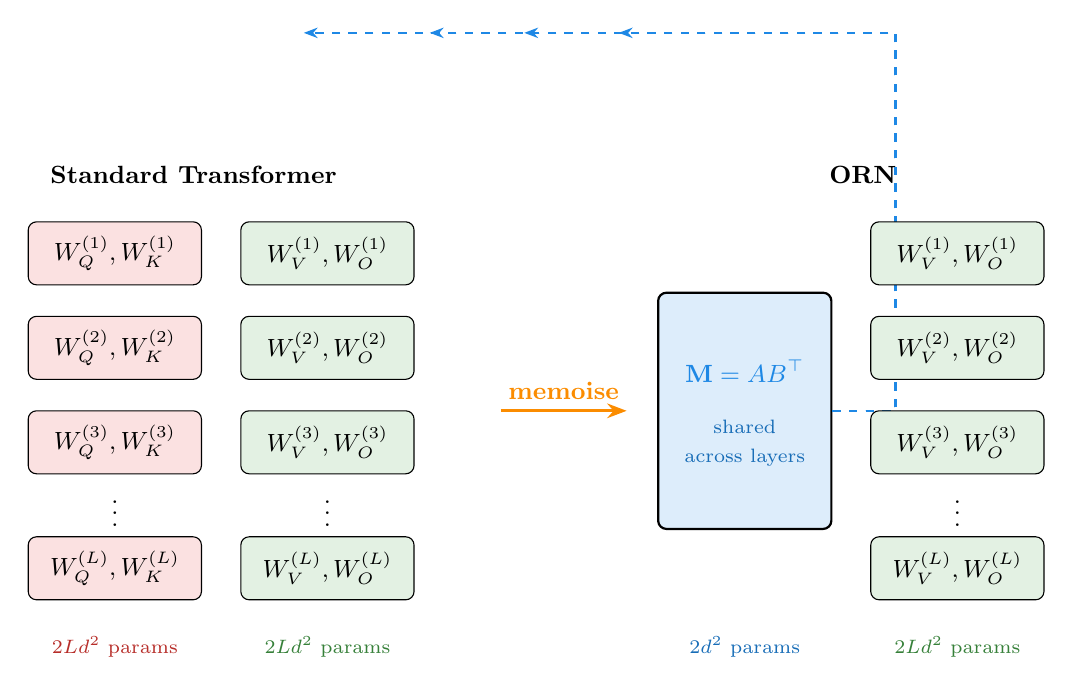
\begin{tikzpicture}[
    layer/.style={draw, rounded corners=3pt, minimum height=0.8cm, minimum width=2.2cm, font=\small},
    shared/.style={draw, rounded corners=3pt, minimum height=0.8cm, minimum width=2.2cm, font=\small, thick, fill=orbitblue!15},
    perlayer/.style={draw, rounded corners=3pt, minimum height=0.8cm, minimum width=2.2cm, font=\small, fill=seedred!15},
    arr/.style={-{Stealth[length=5pt]}, thick},
    bigarr/.style={-{Stealth[length=7pt]}, very thick, dynamicsorange},
]

% Left: Standard transformer
\node[font=\small\bfseries] at (-3.2, 3.2) {Standard Transformer};
\node[perlayer] (L1q) at (-4.2, 2.2) {$W_Q^{(1)}, W_K^{(1)}$};
\node[perlayer] (L2q) at (-4.2, 1.0) {$W_Q^{(2)}, W_K^{(2)}$};
\node[perlayer] (L3q) at (-4.2, -0.2) {$W_Q^{(3)}, W_K^{(3)}$};
\node[font=\small] at (-4.2, -1.0) {$\vdots$};
\node[perlayer] (LLq) at (-4.2, -1.8) {$W_Q^{(L)}, W_K^{(L)}$};

\node[layer, fill=targetgreen!15] (L1v) at (-1.5, 2.2) {$W_V^{(1)}, W_O^{(1)}$};
\node[layer, fill=targetgreen!15] (L2v) at (-1.5, 1.0) {$W_V^{(2)}, W_O^{(2)}$};
\node[layer, fill=targetgreen!15] (L3v) at (-1.5, -0.2) {$W_V^{(3)}, W_O^{(3)}$};
\node[font=\small] at (-1.5, -1.0) {$\vdots$};
\node[layer, fill=targetgreen!15] (LLv) at (-1.5, -1.8) {$W_V^{(L)}, W_O^{(L)}$};

\node[font=\scriptsize, text=seedred!80!black] at (-4.2, -2.8) {$2Ld^2$ params};
\node[font=\scriptsize, text=targetgreen!80!black] at (-1.5, -2.8) {$2Ld^2$ params};

% Arrow in middle
\draw[bigarr] (0.7, 0.2) -- (2.3, 0.2) node[midway, above, font=\small\bfseries, text=dynamicsorange] {memoise};

% Right: ORN
\node[font=\small\bfseries] at (5.3, 3.2) {ORN};
\node[shared, minimum height=3.0cm, minimum width=2.2cm] (Mshared) at (3.8, 0.2) {};
\node[font=\small, text=orbitblue] at (3.8, 0.7) {$\M = AB^\top$};
\node[font=\scriptsize, text=orbitblue!80!black] at (3.8, 0.0) {shared};
\node[font=\scriptsize, text=orbitblue!80!black] at (3.8, -0.4) {across layers};

% Arrows from shared M to layers
\foreach \y in {2.2, 1.0, -0.2, -1.8} {
    \draw[arr, orbitblue, dashed] (Mshared.east) ++(0.0, 0) -- ++(0.8, 0) |- (\y, 5.0);
}

\node[layer, fill=targetgreen!15] (R1v) at (6.5, 2.2) {$W_V^{(1)}, W_O^{(1)}$};
\node[layer, fill=targetgreen!15] (R2v) at (6.5, 1.0) {$W_V^{(2)}, W_O^{(2)}$};
\node[layer, fill=targetgreen!15] (R3v) at (6.5, -0.2) {$W_V^{(3)}, W_O^{(3)}$};
\node[font=\small] at (6.5, -1.0) {$\vdots$};
\node[layer, fill=targetgreen!15] (RLv) at (6.5, -1.8) {$W_V^{(L)}, W_O^{(L)}$};

\node[font=\scriptsize, text=orbitblue!80!black] at (3.8, -2.8) {$2d^2$ params};
\node[font=\scriptsize, text=targetgreen!80!black] at (6.5, -2.8) {$2Ld^2$ params};

\end{tikzpicture}
\caption{Standard transformer (left) vs.\ ORN (right).
The \textcolor{seedred}{per-layer coupling matrices} ($2Ld^2$ parameters) are replaced by a single \textcolor{orbitblue}{shared coupling geometry} $\M = AB^\top$ ($2d^2$ parameters).
The \textcolor{targetgreen!70!black}{per-layer response matrices} are unchanged---different layers still extract different information.}
\label{fig:shared-vs-perlayer}
\end{figure}


% ------------------------------------------------------------------
\subsection{Why Asymmetry Matters}
\label{sec:grn:asymmetry}

The colour matching task is symmetric: if token $A$ matches token $B$'s colour, then $B$ matches $A$'s colour.
Real language is not symmetric.

\paragraph{A concrete example.}
Consider: ``The cat sat on the mat.''
\begin{itemize}[nosep]
    \item ``cat'' should attend to ``The'' (its determiner) $\;\to\;$ $\text{score}(\text{cat} \to \text{The})$ should be \textbf{high}.
    \item ``The'' need not attend strongly to ``cat'' $\;\to\;$ $\text{score}(\text{The} \to \text{cat})$ can be \textbf{low}.
    \item In autoregressive (left-to-right) models, the causal mask enforces an even harder constraint: future tokens \emph{cannot} attend to past tokens' positions that lie ahead of them.
\end{itemize}

A symmetric coupling matrix $\M = LL^\top$ forces $\text{score}(i \to j) = \text{score}(j \to i)$ for all $i, j$.
This is structurally incompatible with autoregressive modelling, where directionality is fundamental.

\paragraph{The fix: $\M = AB^\top$.}
With separate $A$ and $B$ matrices ($A \neq B$):
\begin{align*}
\text{score}(i \to j) &= (\x_i^\top A)(B^\top \x_j) = \x_i^\top A B^\top \x_j \\
\text{score}(j \to i) &= (\x_j^\top A)(B^\top \x_i) = \x_j^\top A B^\top \x_i
\end{align*}
These are not equal in general (unless $AB^\top$ happens to be symmetric).
Token $i$'s ``query-like'' projection uses $A$; token $j$'s ``key-like'' projection uses $B$.
Asymmetry is restored.

\paragraph{A deeper point: why Q and K are two matrices at all.}
It is natural to think that $W_Q$ and $W_K$ serve two purposes: (1)~select a subspace for coupling, and (2)~model asymmetry.
But subspace selection never required two matrices.
A single projection $W \in \R^{r \times d}$ can project both tokens into an $r$-dimensional subspace and compute their dot product there:
\[
\text{score}_{ij} = (Wx_i)^\top(Wx_j) = x_i^\top W^\top W \, x_j
\]
This selects the subspace perfectly well---but $W^\top W$ is symmetric, so $\text{score}_{ij} = \text{score}_{ji}$ always.
The \emph{only} reason attention uses two separate projections is to break this symmetry.
$W_Q$ and $W_K$ exist because the attention graph is directed, not because subspace selection requires two matrices.

This is why $\M = AB^\top$ is the natural shared coupling: $A$ and $B$ provide asymmetry; their rank controls the subspace dimension; and the entire coupling rule is learned once rather than $L$ times.
Of the $2Ld^2$ parameters a standard transformer spends on per-layer $W_Q, W_K$, nearly all are redundantly re-learning the same subspace selection; only the asymmetry and the per-layer orientation (see Section~\ref{sec:spectral-sharing}) vary.

\paragraph{The evidence.}
In Experiment~2 on Shakespeare character-level modelling:

\begin{center}\small
\renewcommand{\arraystretch}{1.2}
\begin{tabular}{@{}lcl@{}}
\toprule
\textbf{Coupling form} & \textbf{Loss} & \textbf{Outcome} \\
\midrule
Per-layer $W_Q, W_K$ (baseline) & 3.09 & --- \\
Shared symmetric $LL^\top$ & 3.4--4.6 & $3$--$50\times$ worse \\
Shared asymmetric $AB^\top$ & 3.03 & \textbf{Beats baseline by 2.6\%} \\
\bottomrule
\end{tabular}
\end{center}

\noindent
Symmetric $\M$ was catastrophically worse.
Switching to $AB^\top$ not only recovered but exceeded the per-layer baseline.
Asymmetry is not an optional refinement---it is essential.

% ------------------------------------------------------------------
\subsection{The Scaling Evidence}
\label{sec:grn:scaling}

A single experiment at one scale could be a fluke.
The real test: does the advantage hold---and grow---across scales?

Experiment~2 compared STORE (per-layer coupling) and MEMOISE (shared $AB^\top$) at five parameter budgets on Shakespeare character-level modelling.
Critically, saved coupling parameters were reinvested in model width, so both models have the \textbf{same total parameter count} at each scale.

\begin{center}\small
\renewcommand{\arraystretch}{1.2}
\begin{tabular}{@{}rrrr@{}}
\toprule
\textbf{Total params} & \textbf{STORE loss} & \textbf{MEMOISE loss} & \textbf{MEMO / STORE} \\
\midrule
27K & 4.441 & 4.461 & 1.005 \\
72K & 3.801 & 3.746 & 0.985 \\
153K & 3.406 & 3.405 & 1.000 \\
285K & 3.091 & 3.032 & 0.981 \\
477K & 2.760 & 2.727 & 0.988 \\
\bottomrule
\end{tabular}
\end{center}

At the smallest scale (27K), MEMOISE is marginally worse---the model is too small for the shared coupling to compensate.
At every scale above 70K, MEMOISE matches or beats STORE.
The ratio consistently favours MEMOISE and the gap widens with scale.

\paragraph{Scaling exponents.}
Fitting power laws $\calL \propto N^{-\beta}$:
\[
\frac{\beta_{\text{MEMOISE}}}{\beta_{\text{STORE}}} = 1.02\times
\]
A $2\%$ steeper scaling exponent means that for every doubling of parameters, MEMOISE gains an extra $2\%$ advantage.
At toy scale this is modest.
But scaling exponents are multiplicative: a $2\%$ advantage per doubling compounds to $\sim$22\% after 10 doublings (1K$\times$ scale-up).

\begin{intuition}
The scaling advantage comes from \emph{reallocation}.
MEMOISE saves $2(L-1)d^2$ coupling parameters and reinvests them in width.
Wider models have more expressive residual streams, which benefit all layers---including the shared coupling.
The shared coupling is a better inductive bias that \emph{also} frees parameters for the parts that actually need to vary.
\end{intuition}

% ------------------------------------------------------------------
\subsection{The Decomposition: Generator $\times$ Response $\times$ Field}
\label{sec:grf:decomposition}

Before writing code, we need to see the architecture as a \emph{decomposition} of what standard attention does.

\paragraph{Standard attention at layer $l$.}
The residual stream $\x$ enters.
The layer looks up stored matrices $W_Q^{(l)}, W_K^{(l)}$ (the coupling) and $W_V^{(l)}, W_O^{(l)}$ (the response).
It computes attention, adds the result back to $\x$, and passes the updated stream to layer $l{+}1$.

Every layer has its own coupling matrices.
The coupling ``rule'' is re-specified from scratch at each layer.
The residual stream is just a carrier---it passes through, but the rules acting on it change at every step.

\paragraph{The ORN decomposition.}
In the Orbital Response Network, standard attention decomposes into three distinct components:

\begin{enumerate}
    \item \textbf{The generator $\M = AB^\top$} (shared, the world model).
    This is the coupling geometry---it defines which tokens should attend to which.
    It is the \emph{same matrix at every layer}.
    It encodes the structural rules of the domain: ``characters couple with actions,''
    ``determiners couple with nouns.''
    $\M$ is not applied once---it is the \textbf{generator of an orbit}.
    Applied repeatedly to an evolving state, it produces a trajectory through coupling space.
    Mathematically, $\M$ generates a \emph{semigroup}: the operation ``apply $\M$-based coupling then respond'' can be composed arbitrarily ($s$ steps followed by $t$ steps $=$ $s{+}t$ steps), and this composition is associative.
    The generator is a compact description---one matrix---that unfolds into arbitrarily long trajectories.

    \item \textbf{The response heads $W_V^{(l)}, W_O^{(l)}$} (per-layer, the interaction).
    These define how each layer \emph{reads from} and \emph{writes to} the residual stream
    given the coupling pattern that $\M$ produced.
    Layer 1 might extract raw features; layer 4 might extract refined semantic roles.
    The \emph{what} changes per layer; the \emph{who-talks-to-whom} does not.

    \item \textbf{The residual stream} (evolving, the orbit).
    This is the state that flows through the network.
    At each layer, $\M$ acts on the \emph{current} residual state to produce coupling.
    The response heads modify the state.
    The state enters the next layer, where $\M$ acts again.

    The residual stream \textbf{is the orbit}---the trajectory of the representation
    under repeated application of the shared generator $\M$ and the per-layer responses.

    We call this the \emph{stigmergic residual}.
    In stigmergic systems (ant colonies, termite mounds), simple agents make locally optimal decisions by reading and writing to a shared medium---the environment itself carries the coordination signal.
    No ant knows the global plan; each responds to pheromone gradients, and collective intelligence emerges in the field.

    The residual stream is the pheromone trail.
    Each layer's response heads are the ants---simple, local, per-layer.
    They read the current state of the residual (the field), respond via $W_V^{(l)}, W_O^{(l)}$, and write their contribution back.
    The coupling geometry $\M$ determines how the field mediates interaction between tokens, just as pheromone diffusion determines how the environment mediates interaction between ants.
    Cognition is not in the response heads; \textbf{it is in the field}.
    The response heads are simple; the residual stream, shaped by $\M$, is where the structure accumulates.

    This is what makes the architecture scalable: adding more layers (more ants) does not require more coupling rules---only more local responses to the same shared field.
\end{enumerate}

\paragraph{Why ``orbit'' and ``generator''?}
In the mathematics of dynamical systems, a \emph{generator} is an operator that, when applied repeatedly, produces a trajectory (an \emph{orbit}).
If $\M$ is the generator, then the sequence:
\[
    \x_0 \;\xrightarrow{\;\M, V^{(1)}, O^{(1)}\;}\; \x_1 \;\xrightarrow{\;\M, V^{(2)}, O^{(2)}\;}\; \x_2 \;\xrightarrow{\;\M, V^{(3)}, O^{(3)}\;}\; \cdots
\]
is the orbit of $\x_0$ under $\M$.
This is a \emph{semigroup} action: the composition of ``apply $\M$ then respond'' at step $s$ and step $t$ is the same as applying it for $s{+}t$ steps.
The generator is fixed; the state evolves; the orbit unfolds.

\paragraph{What this replaces.}
In a standard transformer, the coupling at each layer is a \emph{memory lookup}: load $W_Q^{(l)}, W_K^{(l)}$ from storage (indexed by layer number $l$).
In the ORN, the coupling is a \emph{computation}: apply the shared $\M$ to the current residual state.
The lookup is replaced by running the generator.
The stored coupling matrices are replaced by one shared generator and an evolving orbit.

\begin{figure}[h]
\centering
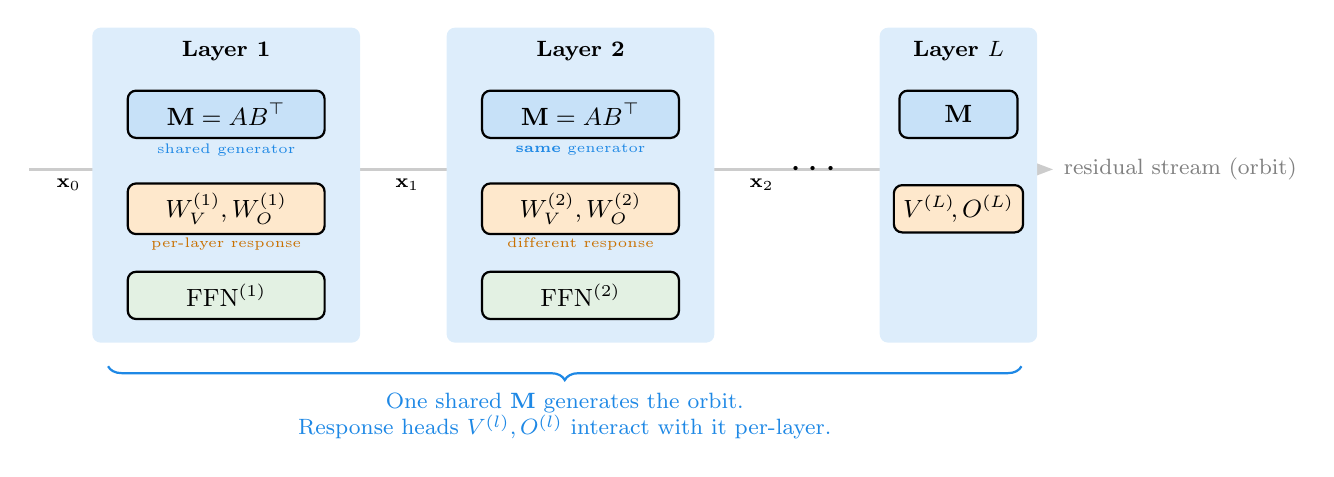
\begin{tikzpicture}[>=Stealth, font=\small, node distance=1.2cm]
    % Residual stream (the orbit)
    \draw[very thick, gray!40, ->] (-0.5, 0) -- (12.5, 0)
        node[right, font=\footnotesize, gray] {residual stream (orbit)};

    % Layer 1
    \fill[orbitblue!15, rounded corners=3pt] (0.3, -2.2) rectangle (3.7, 1.8);
    \node[font=\footnotesize\bfseries] at (2, 1.5) {Layer 1};

    \node[draw, thick, fill=orbitblue!25, rounded corners=3pt,
          minimum width=2.5cm, minimum height=0.6cm] (M1) at (2, 0.7) {$\M = AB^\top$};
    \node[font=\tiny, orbitblue] at (2, 0.25) {shared generator};

    \node[draw, thick, fill=dynamicsorange!20, rounded corners=3pt,
          minimum width=2.5cm, minimum height=0.6cm] (R1) at (2, -0.5) {$W_V^{(1)}, W_O^{(1)}$};
    \node[font=\tiny, dynamicsorange!80!black] at (2, -0.95) {per-layer response};

    \node[draw, thick, fill=targetgreen!15, rounded corners=3pt,
          minimum width=2.5cm, minimum height=0.6cm] (F1) at (2, -1.6) {FFN$^{(1)}$};

    % Layer 2
    \fill[orbitblue!15, rounded corners=3pt] (4.8, -2.2) rectangle (8.2, 1.8);
    \node[font=\footnotesize\bfseries] at (6.5, 1.5) {Layer 2};

    \node[draw, thick, fill=orbitblue!25, rounded corners=3pt,
          minimum width=2.5cm, minimum height=0.6cm] (M2) at (6.5, 0.7) {$\M = AB^\top$};
    \node[font=\tiny, orbitblue] at (6.5, 0.25) {\textbf{same} generator};

    \node[draw, thick, fill=dynamicsorange!20, rounded corners=3pt,
          minimum width=2.5cm, minimum height=0.6cm] (R2) at (6.5, -0.5) {$W_V^{(2)}, W_O^{(2)}$};
    \node[font=\tiny, dynamicsorange!80!black] at (6.5, -0.95) {different response};

    \node[draw, thick, fill=targetgreen!15, rounded corners=3pt,
          minimum width=2.5cm, minimum height=0.6cm] (F2) at (6.5, -1.6) {FFN$^{(2)}$};

    % Dots
    \node[font=\Large] at (9.5, 0) {$\cdots$};

    % Layer L
    \fill[orbitblue!15, rounded corners=3pt] (10.3, -2.2) rectangle (12.3, 1.8);
    \node[font=\footnotesize\bfseries] at (11.3, 1.5) {Layer $L$};
    \node[draw, thick, fill=orbitblue!25, rounded corners=3pt,
          minimum width=1.5cm, minimum height=0.6cm] at (11.3, 0.7) {$\M$};
    \node[draw, thick, fill=dynamicsorange!20, rounded corners=3pt,
          minimum width=1.5cm, minimum height=0.6cm] at (11.3, -0.5) {$V^{(L)}\!,O^{(L)}$};

    % State labels
    \node[font=\scriptsize, below] at (0, 0) {$\x_0$};
    \node[font=\scriptsize, below] at (4.3, 0) {$\x_1$};
    \node[font=\scriptsize, below] at (8.8, 0) {$\x_2$};

    % Brace for M
    \draw[decorate, decoration={brace, amplitude=5pt, mirror}, thick, orbitblue]
        (0.5, -2.5) -- (12.1, -2.5)
        node[midway, below=6pt, font=\footnotesize, orbitblue, align=center]
        {One shared $\M$ generates the orbit.\\Response heads $V^{(l)}, O^{(l)}$ interact with it per-layer.};

\end{tikzpicture}
\caption{\textbf{The ORN decomposition.}
The residual stream (grey arrow) is the orbit---the trajectory of the representation.
At each layer, the \textcolor{orbitblue}{same generator $\M$} computes coupling
(who attends to whom), while \textcolor{dynamicsorange!80!black}{per-layer response heads}
determine what information flows.
$\M$ is the world model; the response heads are the interaction mechanism;
the residual stream is the orbit they jointly produce.}
\label{fig:grn-decomposition}
\end{figure}

\begin{intuition}
Think of the residual stream as a ball rolling across a landscape.
$\M$ defines the landscape---the hills, valleys, and slopes that determine which
directions are ``downhill'' (high coupling) and which are ``uphill'' (low coupling).
The landscape is fixed (shared $\M$).
The ball's position changes at each step (the evolving residual state).
The response heads are like guardrails that deflect the ball at specific points---
different guardrails at each layer, but the same landscape throughout.

A standard transformer redraws the entire landscape at each step.
The ORN says: the landscape doesn't change---only the ball's position does.
\end{intuition}

\paragraph{Example: signal processing.}
Consider a multi-stage audio filter that processes a mixture of frequencies.
The coupling rule is: ``attend to samples at the same frequency.''
This rule is the same at every stage---what changes is the signal itself (it gets progressively cleaner).

\begin{itemize}[nosep]
    \item \textbf{Generator $\M$:} the frequency-coupling matrix.
          ``Same frequency $\to$ high coupling, different frequency $\to$ low coupling.''
          Identical at every stage.
    \item \textbf{Response (stage 1):} extract raw amplitude from coupled samples.
    \item \textbf{Response (stage 3):} extract refined phase-corrected signal.
    \item \textbf{Orbit:} the signal evolves from noisy mixture $\to$ clean components.
\end{itemize}
You do not need a different frequency-coupling rule at stage 3.
The coupling (``same frequency $\to$ attend'') is the generator.
What you \emph{do with} the attended signal changes per stage.

\paragraph{Example: TinyStories.}
``Lily wanted the cake.'' Processed by a 4-layer ORN:

\begin{itemize}[nosep]
    \item \textbf{Generator $\M$:} the structural coupling rule.
          ``CHAR couples with ACTION, DET couples with OBJ.''
          Same at every layer.
    \item \textbf{Response (layer 1):} $W_V^{(1)}$ extracts raw token features.
          ``Lily'' $\to$ \emph{some entity}, ``wanted'' $\to$ \emph{some action}.
          The response is shallow: surface-level feature extraction.
    \item \textbf{Response (layer 3):} $W_V^{(3)}$ extracts refined compositional meaning.
          ``Lily wanted'' $\to$ \emph{agent-desires-object}.
          Same coupling pattern (CHAR$\to$ACTION), but the response now captures the composed meaning.
    \item \textbf{Orbit:} the residual stream evolves from raw embeddings $\to$ contextualised representations.
          At layer 0: ``Lily'' is just a name.
          By layer 3: ``Lily'' carries ``agent who desires cake''---information routed by $\M$ from ``wanted'' and ``cake.''
\end{itemize}

The key: at both layer 1 and layer 3, $\M$ says ``Lily should attend to wanted.''
What \emph{flows through} that attention link differs because $W_V^{(1)} \neq W_V^{(3)}$.
Same generator, same coupling, different response, evolving orbit.

\paragraph{What is proven and what is not.}
The decomposition rests on three empirical claims, each with evidence:

\begin{enumerate}[nosep]
    \item \textbf{The generator is approximately invariant across layers.}
    Proven: eigenspectrum correlation 0.96--0.99 on learned matrices
    (Section~\ref{sec:grn:micro-language}: micro-language;
    Section~\ref{sec:grn:exp0}: Exp~0 on structured sequences).
    The spectral \emph{shape} of $M_l$ is the same at every layer, even though the raw matrices differ.

    \item \textbf{Sharing one $\M$ works without quality loss.}
    Proven: Exp~1 (Section~\ref{sec:grn:share}): MEMOISE with shared $\M$ beats STORE with per-layer $W_Q, W_K$ by 0.7\%, using 16$\times$ fewer coupling parameters.
    Exp~2 (Section~\ref{sec:grn:scaling}): MEMOISE matches or beats STORE at every scale above 70K parameters.

    \item \textbf{Response heads must stay per-layer.}
    Proven: Exp~1: MEMOISE+TIED (shared response) loses 4.1\%.
    The coupling rule is invariant; the response is not.
    This validates the split: share the generator, keep the responses per-layer.

    \item \textbf{The full decomposition is visible on a trained GRF.}
    We trained a 4-layer GRF (shared $A, B$, per-layer $V, O$) on the micro-language and traced ``Lily wanted the cake'' through every layer, recording the coupling pattern, the value extraction, and the residual stream at each step.

    \begin{center}\small
    \renewcommand{\arraystretch}{1.2}
    \begin{tabular}{@{}lrl@{}}
    \toprule
    \textbf{Component} & \textbf{Cross-layer similarity} & \textbf{Expected} \\
    \midrule
    Coupling (shared $\M$) & \textbf{0.94} & High (same M) \\
    Response (per-layer $V$) & \textbf{$-$0.03} & Low (different V) \\
    Orbit (residual stream) & evolving & Changes each layer \\
    \bottomrule
    \end{tabular}
    \end{center}

    The three components separate cleanly on learned weights.
    The shared $\M$ produces coupling patterns with 0.94 cross-layer cosine similarity.
    The per-layer responses are essentially uncorrelated ($-0.03$): each layer extracts completely different information through the same coupling pattern.
    The residual stream evolves progressively through the layers.

    Comparing ``Lily wanted the cake'' and ``Emma wanted the ball'' through the same GRF: coupling cosine ranges from 0.967 (layer~0) to 0.999 (layer~3).
    The shared $\M$ treats them as structurally equivalent, with the similarity \emph{increasing} at deeper layers as the representations become more role-abstracted.
\end{enumerate}

\paragraph{The practical consequence.}
This decomposition tells you exactly what to share and what to keep per-layer:
\begin{center}\small
\renewcommand{\arraystretch}{1.3}
\begin{tabular}{@{}lll@{}}
\toprule
\textbf{Component} & \textbf{Role} & \textbf{Sharing} \\
\midrule
$A, B$ (coupling) & The generator: which relationships matter & \textbf{Shared} across all layers \\
$W_V^{(l)}$ & What to extract from attended tokens & Per-layer \\
$W_O^{(l)}$ & How to write back to the residual stream & Per-layer \\
FFN$^{(l)}$ & Per-token nonlinear transform & Per-layer \\
Residual stream & The orbit: evolving state & Flows through \\
\bottomrule
\end{tabular}
\end{center}

\noindent
The \textbf{world model} ($\M$) is shared because the rules of coupling don't change with depth.
The \textbf{responses} ($V, O$, FFN) vary because different depths extract and transform different information.
The \textbf{orbit} (residual stream) evolves because each layer adds its contribution.

This is the full story of what ``orbital'' means in the ORN:
$\M$ generates the orbit; the residual stream \emph{is} the orbit; the response heads ride it.

% ------------------------------------------------------------------
\subsection{Building the ORN in PyTorch}
\label{sec:grn:pytorch}

Now that we understand \emph{why} the architecture works, here is the \emph{how}.

\begin{lstlisting}[caption={ORN attention layer: shared coupling, per-layer response}]
class ORNAttention(nn.Module):
    def __init__(self, d_model, n_heads, shared_A, shared_B):
        super().__init__()
        # shared_A and shared_B are REFERENCES, not copies.
        # Every layer points to the same tensor.
        # When gradients flow back, they all update the same A and B.
        self.A = shared_A    # shape: (d_model, d_model)
        self.B = shared_B    # shape: (d_model, d_model)

        # Per-layer response (these ARE different per layer)
        self.Wv = nn.Linear(d_model, d_model, bias=False)
        self.Wo = nn.Linear(d_model, d_model, bias=False)
        self.d_head = d_model // n_heads

    def forward(self, x, causal_mask):
        # Coupling: same A, B at every layer
        q = x @ self.A          # (batch, seq, d_model)
        k = x @ self.B          # (batch, seq, d_model)

        # Scaled dot-product attention
        scores = (q @ k.transpose(-2, -1)) / (self.d_head ** 0.5)
        scores = scores.masked_fill(causal_mask, float('-inf'))
        attn = torch.softmax(scores, dim=-1)

        # Response: per-layer V and O
        v = self.Wv(x)
        return self.Wo(attn @ v)
\end{lstlisting}

\paragraph{Line-by-line.}
\begin{itemize}[nosep]
    \item \texttt{self.A = shared\_A} --- this is a Python reference assignment, not a copy.
    Every layer's \texttt{self.A} points to the \emph{same} \texttt{nn.Parameter} tensor.
    During backpropagation, gradients from all $L$ layers accumulate into this single tensor.
    \item \texttt{q = x @ self.A} --- the ``query-like'' projection, shared across layers.
    \item \texttt{k = x @ self.B} --- the ``key-like'' projection, shared across layers.
    \item \texttt{self.Wv}, \texttt{self.Wo} --- these are \emph{not} shared.
    Each layer has its own response matrices because different depths extract different features.
\end{itemize}

The model constructor creates $A$ and $B$ once and passes references:

\begin{lstlisting}[caption={Model constructor: creating shared coupling once}]
class ORNTransformer(nn.Module):
    def __init__(self, d_model, n_layers, n_heads):
        super().__init__()
        # ONE shared coupling geometry for the whole model
        self.A = nn.Parameter(torch.randn(d_model, d_model) * 0.02)
        self.B = nn.Parameter(torch.randn(d_model, d_model) * 0.02)

        # L layers, each with per-layer V, O but shared A, B
        self.layers = nn.ModuleList([
            ORNBlock(d_model, n_heads,
                     shared_A=self.A,   # same tensor
                     shared_B=self.B)   # same tensor
            for _ in range(n_layers)
        ])
\end{lstlisting}

\noindent
Note: \texttt{self.A} and \texttt{self.B} are \texttt{nn.Parameter} objects owned by the top-level model.
The individual \texttt{ORNBlock} layers hold references, not copies.
PyTorch's autograd handles the rest---gradients from every layer flow into the single shared $A$ and $B$.

% ------------------------------------------------------------------
\subsection{The Spectral Sharing Insight}
\label{sec:grn:spectral}
\label{sec:spectral-sharing}

The Exp~0 results contained a deeper clue.
The coupling matrices $M_l$ had near-identical eigenspectra but different eigenvectors.
To understand what this means---and why it matters---we need to unpack what eigenvalues and eigenvectors mean in the context of language processing.

\paragraph{What eigenvalues mean in language.}
Each eigenvalue of the coupling matrix defines a \emph{type} of relationship and how important that type is.
In a trained model on language data, the eigenspectrum encodes something like:
\begin{itemize}[nosep]
    \item $\lambda_1$ (large): \textbf{syntactic adjacency}---determiners attend to nouns, subjects to verbs.
    \item $\lambda_2$ (large): \textbf{semantic role}---characters attend to their actions (``Lily'' $\leftrightarrow$ ``wanted'').
    \item $\lambda_3$ (medium): \textbf{coreference}---pronouns attend to antecedents (``she'' $\to$ ``Lily'').
    \item $\lambda_{4\text{--}d}$ (small): fine-grained distinctions---tense agreement, modifier scope, etc.
\end{itemize}
The spectral invariance (0.98 correlation across layers) means: \textbf{all layers agree on WHICH relationship types matter and how much.}
Layer~1 and layer~8 both say ``syntactic adjacency is the strongest coupling, semantic role is second, coreference is third.''
The grammar of English does not change at layer~5.

\begin{remark}
\textbf{Realisation: The coupling manifold is 8-dimensional (\#96).}
PCA of attention patterns from GPT-2 reveals that all coupling lives in an $\sim$8-dimensional manifold, despite the nominal coupling matrices being $768 \times 768$.
In our ORN with shared $\M$, the manifold is even tighter: 5--7 dimensions.
Transformers spend $\sim$25\% of parameters navigating a space with fewer than 10 effective dimensions~\cite{masa2025}.
This is why sharing works---there is almost nothing there to begin with.
\end{remark}

\paragraph{What eigenvectors mean in language.}
The eigenvectors say \emph{where in the embedding space} each relationship type lives.
And this is where layers differ.

Consider ``The'' at layer~1: its determiner-ness lives in dimensions 1--3 of the residual stream.
At layer~5, after four layers of transformation, determiner-ness has been mixed into dimensions 12--18.
The coupling rule is the same---``determiners couple with nouns strongly''---but the \emph{coordinates} of ``determiner'' and ``noun'' in the residual stream have rotated.

It is the same rule written in different coordinate frames.

\begin{intuition}
The coupling matrix encodes the grammar of attention---which relationships matter.
The grammar does not change between layers; only the coordinate frame does.
\end{intuition}

\paragraph{What this means concretely.}

\begin{center}\small
\renewcommand{\arraystretch}{1.3}
\begin{tabular}{@{}p{3cm}p{5cm}p{5cm}@{}}
\toprule
& \textbf{Eigenvalues (shared)} & \textbf{Eigenvectors (per-layer)} \\
\midrule
What it encodes & ``Determiners couple with nouns strongly, semantic roles couple moderately'' & ``In THIS layer's frame, determiner-ness is along dims $X, Y, Z$'' \\
Why invariant? & The grammar of English does not change at layer 5 & --- \\
Why varies? & --- & The residual stream rotates through processing \\
\bottomrule
\end{tabular}
\end{center}

\paragraph{Three strategies as a progression.}
The CPU gap tests compared sharing strategies, which form a natural progression:

\begin{description}[nosep]
    \item[Full sharing (current ORN):] One matrix $\M$, $d^2$ parameters.
    Gradient descent finds the best compromise orientation across all layers.
    Works---but not optimal, because the compromise orientation is wrong for every individual layer.

    \item[Spectral sharing:] Shared eigenvalues $\bar{\Lambda}$ $+$ per-layer rotation matrices $R_l$.
    Each layer gets $M_l = R_l \bar{\Lambda} R_l^\top$.
    Error reduction: \textbf{99.9\%} compared to full sharing.
    But per-layer rotations are expensive: $L \times d^2$ parameters for the rotations, partially defeating the purpose.

    \item[Low-rank corrections:] Shared mean $\bar{M}$ $+$ per-layer rank-$r$ residual $U_l V_l^\top$.
    Error reduction: 37\% at rank 2.
    Cost: $d^2 + L \times 2rd$ --- moderate.
\end{description}

\paragraph{A tempting hypothesis: smooth rotations.}
If the residual stream changes \emph{gradually} between layers, perhaps the eigenvector rotations change gradually too---forming a smooth path through the rotation group.
If so, we could store a single ``angular velocity'' generator $\omega$ and compute all rotations as $R_l = R_0 \cdot \exp(l \cdot \omega)$.
This would be extremely cheap: $\sim 1.5d^2$ parameters, \textbf{independent of $L$}.

The analogy: instead of 8 photographs of a mountain from random angles, imagine a camera slowly panning around the mountain.
Each frame is a small rotation from the last.
You could reconstruct all 8 frames from the starting position and the pan speed.

\paragraph{We tested this. It failed.}
We trained an 8-layer transformer on TinyStories and extracted the inter-layer rotations $\delta R_l = R_{l+1} R_l^\top$ between consecutive layers' eigenvectors.

\begin{center}\small
\renewcommand{\arraystretch}{1.2}
\begin{tabular}{@{}lrl@{}}
\toprule
\textbf{Test} & \textbf{Result} & \textbf{Verdict} \\
\midrule
Mean cosine between $\delta R$ pairs & $-0.003 \pm 0.017$ & Random (no consistency) \\
Deviation from mean $\delta R$ & 2.47 & Very large \\
Single-generator reconstruction & 0.10 mean $|\cos|$ & Near chance (0.08 = random) \\
\bottomrule
\end{tabular}
\end{center}

\noindent
The inter-layer rotations are \textbf{completely unrelated to each other}.
There is no smooth path, no semigroup, no single generator.
The photographs-of-a-mountain analogy was right about the shape being shared (eigenvalues), but wrong about the camera: the camera teleports to a random angle at each layer, it does not pan smoothly.

\paragraph{Why this makes sense, in retrospect.}
Each transformer layer adds a residual: $\x_{l+1} = \x_l + f_l(\x_l)$.
While the residual is ``small'' relative to $\x_l$, each layer's function $f_l$ has \emph{different weights} ($W_V^{(l)}, W_O^{(l)}$, FFN$^{(l)}$).
The per-layer response heads rotate the residual stream in directions that are \emph{task-dependent}, not geometrically smooth.
Layer~3 might push entity representations into one subspace; layer~4 might push syntactic features into an orthogonal subspace.
These are unrelated rotations driven by different per-layer objectives.

\paragraph{What survives.}
\begin{itemize}[nosep]
    \item \textbf{Eigenvalue sharing: confirmed.} The shape of the coupling landscape is consistent across layers.
    \item \textbf{Full matrix sharing (current ORN): works.} Gradient descent finds a single $\M$ that is a good-enough compromise.
    \item \textbf{Smooth rotation sharing: falsified.} The per-layer orientations are random---no cheap generator exists.
    \item \textbf{Low-rank corrections: the practical middle ground.} Rank-2 per-layer corrections give 37\% error reduction at moderate cost.
\end{itemize}

\begin{center}\small
\renewcommand{\arraystretch}{1.2}
\begin{tabular}{@{}lrrl@{}}
\toprule
\textbf{Strategy} & \textbf{Error reduction} & \textbf{Coupling params} & \textbf{Status} \\
\midrule
Full sharing ($\M$) & baseline & $d^2$ & Validated (Exp 1, 2) \\
Low-rank correction ($\bar{M} + U_l V_l^\top$) & 37\% & $d^2 + 2Lrd$ & CPU validated \\
Spectral sharing ($R_l \bar{\Lambda} R_l^\top$) & 99.9\% & $d + Ld^2$ & CPU validated (expensive) \\
Semigroup generator ($R_0 e^{l\omega}$) & --- & $1.5d^2$ & \textbf{Falsified} \\
\bottomrule
\end{tabular}
\end{center}

\begin{intuition}
The coupling rule has a shared \emph{shape} (eigenvalues) but random \emph{orientations} (eigenvectors) across layers.
This is why full sharing works: gradient descent finds the best compromise shape.
But there is no deeper geometric structure connecting the orientations---they are determined by the per-layer response heads, which have independent weights.
The good news: full sharing already captures the essential geometry.
The orientations are noise on top of the shared shape, and the model tolerates losing them.
\end{intuition}

\paragraph{Why the ORN may get the rotation for free.}
The falsification of smooth rotation sharing seems like bad news: we cannot cheaply parameterise the per-layer orientations.
But there is a deeper reason this may not matter.

\emph{Why} do eigenvectors rotate across layers?
Because the response heads ($W_V^{(l)}, W_O^{(l)}$) and FFNs \emph{modify the residual stream} at each layer.
The residual stream is the coordinate system in which the shared $\M$ operates.
When layer 5's response heads update the residual stream, they rotate the coordinates that layer 6 will use.
The per-layer eigenvector rotation is not an independent parameter---it is a \emph{consequence} of the content updates that the response heads perform.

This means the ORN's architecture already has a mechanism for producing per-layer rotation: \textbf{the response heads create it as a side effect of their primary job}.
When we share $\M$ and keep per-layer $W_V, W_O$, the response heads simultaneously:
\begin{enumerate}[nosep]
    \item Transform the \emph{content} flowing through the residual stream (their explicit job).
    \item Rotate the \emph{coordinate frame} in which the shared coupling will be evaluated at the next layer (an implicit side effect).
\end{enumerate}
The coupling rule is fixed; the residual field evolves under it.
The response heads don't need to ``know'' about the rotation---they produce it naturally by updating the field that the shared coupling acts upon.

Whether this emergent rotation is \emph{sufficient}---or whether a cheap explicit per-layer correction would help---is an empirical question for future work.
But the architectural insight is clear: the shared coupling and per-layer response are not independent systems.
The response shapes the field; the field determines how the coupling is expressed.
They co-evolve through this shared geometric medium, which is the residual stream itself.

\begin{remark}
\textbf{Realisation: WSD decay improves loss without changing M (\#167).}
In our 108M V2 model, the WSD learning rate decay phase dropped val loss from 3.19 to 3.01 nats---a 0.23 nat improvement---while $\M$'s spectral structure barely changed (rank $71 \to 69$, asymmetry $1.413 \to 1.411$).
The decay improved \emph{only the response heads} while $\M$ stayed geometrically fixed.
This is the strongest evidence that coupling and response are genuinely independent systems: you can improve one without touching the other.
\end{remark}

\begin{remark}
\textbf{Realisation: ORN beats GPT-2 + SmolLM on 5/8 benchmarks (\#169).}
At 108M parameters and 8B tokens (2.7\% of GPT-2's training data), the ORN-V2 beats both GPT-2 Small (124M, 300B tokens) and SmolLM-135M (135M, 600B tokens) on 5 of 8 zero-shot benchmarks, averaging 41.8\% vs 40.2\% and 40.1\%.
The strongest wins are on structural reasoning tasks (HellaSwag, ARC) where shared coupling geometry provides an architectural advantage.
\end{remark}

% ------------------------------------------------------------------
\subsection{Putting Both Tables Together}
\label{sec:grn:full-picture}

We can now see the complete picture: both the embedding table (Table~1, Section~\ref{sec:orbital-embed}) and the attention projections (Table~2, this section) memoised.

\begin{center}\small
\renewcommand{\arraystretch}{1.3}
\begin{tabular}{@{}lll@{}}
\toprule
\textbf{Component} & \textbf{Standard Transformer} & \textbf{Full ORN} \\
\midrule
Token input & Lookup table ($V \times d$) & Seeds + $\Phi$ ($V \times d_s + |\Phi|$) \\
Coupling & Per-layer $W_Q, W_K$ ($2Ld^2$) & Shared $\M = AB^\top$ ($2d^2$) \\
Response & Per-layer $W_V, W_O$ ($2Ld^2$) & Per-layer $W_V, W_O$ ($2Ld^2$) \\
FFN & Per-layer ($\sim 8Ld^2$) & Shared wide ($\sim 8d^2$, V3) or per-layer ($\sim 8Ld^2$, V2) \\
Token output & Tied with embedding ($V \times d$) & Via seed space ($d \times d_s + V \times d_s$) \\
\bottomrule
\end{tabular}
\end{center}

\noindent
At GPT-2 scale ($V = 50\text{K}$, $d = 768$, $L = 12$):
\begin{itemize}[nosep]
    \item Embedding: $38.4\text{M} \to 2.6\text{M}$ ($14.8\times$ compression)
    \item Coupling: $14.2\text{M} \to 1.2\text{M}$ ($12\times$ compression)
    \item \textbf{Total saved: $\sim$49M params} (40\% of the 124M model)
\end{itemize}

\noindent
These freed parameters can be reinvested in model width, more response heads, or deeper FFNs---the parts that actually need to vary per layer.

\begin{intuition}
The design principle is the same throughout: if a computation is approximately the same across instances (tokens for embeddings, layers for coupling), \textbf{share the parameters and compute rather than store}.
What varies is the \emph{input} to the shared computation, not the computation itself.
\end{intuition}

\begin{remark}
\textbf{Realisation: Wide shared FFN beats per-layer at matched params (\#178).}
ORN V3 extends the sharing to the FFN: one $L\times$-wider shared FFN replaces $L$ per-layer FFNs at the same parameter count.
Experimentally, this \emph{beats} the per-layer baseline by 0.8\%~\cite{onewideffn2023, ffnfusion2025}.
The FFN stores key-value memories (facts and patterns)~\cite{geva2021ffn}---and one wide shared memory has more capacity than $L$ narrow copies.
With both $\M$ and FFN shared, $\sim$78\% of the model is universal backbone; only $\sim$22\% (response heads + corrections) is per-layer.
At GPT-2 scale, this means a 61M ORN-V3 matches a 124M transformer---half the parameters.
\end{remark}


% ======================================================================
\section{How Context Flows: The Residual Stream as Communication Bus}
\label{sec:residual-flow}

Before looking ahead, we need to understand how information actually moves through a transformer (or an ORN).
This is the foundation for understanding why the ORN's shared geometry works, why state breaks composition, and how layers interact.

\subsection{The Residual Stream}

A transformer processes tokens through $L$ layers.
Each layer reads the hidden state, transforms it, and writes the result back.
The critical mechanism is the \textbf{residual connection}~\cite{he2016deep}: the output of each layer is \emph{added} to its input, not replacing it.

\begin{align}
    h^{(0)} &= \text{embed}(\text{tokens}) \\
    h^{(1)} &= h^{(0)} + \text{Attn}_1(h^{(0)}) + \text{FFN}_1(\ldots) \\
    h^{(2)} &= h^{(1)} + \text{Attn}_2(h^{(1)}) + \text{FFN}_2(\ldots) \\
    &\vdots
\end{align}

Because each layer \emph{adds} to the previous state, the hidden state $h^{(\ell)}$ at layer $\ell$ contains contributions from \emph{all} previous layers:
\[
    h^{(\ell)} = h^{(0)} + \sum_{k=0}^{\ell-1} \Delta_k
\]
where $\Delta_k$ is what layer $k$ wrote.
Layer~10 can still ``read'' what layer~1 wrote, because it is still present in $h^{(10)}$ via the residual chain.

\subsection{Sequential, Parallel, and Persistent}

Information flow is three things at once:

\begin{itemize}[nosep]
    \item \textbf{Sequential between layers}: layer~5 reads the output of layers 0--4.
    It cannot see layer~6's contribution (that hasn't been written yet).
    \item \textbf{Parallel within a layer}: all attention heads at the same layer read the same $h^{(\ell)}$ simultaneously and write back in parallel.
    No head ``goes first.''
    \item \textbf{Persistent across depth}: the residual connection means early layers' contributions persist.
    Information written at layer~1 is still in the stream at layer~12.
    It may be diluted (overwritten by later contributions) but it is never erased.
\end{itemize}

The residual stream functions as a \textbf{communication bus}: a shared medium that all layers read from and write to.
Specific ``circuits'' form across layers---the output of head $A$ at layer~3 may be specifically read by head $B$ at layer~7 via the bus.

\subsection{How This Maps to the ORN}

In the ORN, the residual stream is the \textbf{field state}---the medium through which all agents interact:

\begin{itemize}[nosep]
    \item $\M$ defines the \textbf{bus protocol}: which tokens' contributions each agent can see (the coupling geometry).
    The same protocol at every layer.
    \item \textbf{Response heads} are agents that read the bus (via $\M$'s coupling), transform what they read (via $W_V, W_O$, FFN), and write the result back to the bus.
    Each agent is independent; each reads the same field state.
    \item \textbf{Perturbative corrections} handle bus noise---information that doesn't fit $\M$'s protocol.
    They are small, gated, and active mainly at late layers where the coupling diverges most from the shared geometry.
    \item \textbf{There is no other memory.}
    The residual stream carries everything.
    This is why separate state tensors (like the delta-rule accumulator) break composition: they add a parallel bus outside $\M$'s geometry.
    Gradient descent routes information through whichever bus is easier, and the separate bus bypasses $\M$, destroying the shared geometry.
\end{itemize}

The ORN's design principle: \textbf{one bus, one protocol ($\M$), many agents (response heads)}.
All information flows through the residual stream, governed by $\M$'s coupling.
No side channels.

\subsection{Why Per-Layer Variation Comes From the Stream, Not From the Parameters}

This is the key insight.
In a standard transformer, each layer has different $W_Q^{(\ell)}, W_K^{(\ell)}$, so the coupling changes with depth.
But the residual stream $h^{(\ell)}$ \emph{also} changes with depth---each layer's response heads update it.

In the ORN, the coupling ($\M$) is fixed.
The \emph{field state} ($h^{(\ell)}$) evolves.
The same $\M$ applied to different $h^{(\ell)}$ produces different coupling patterns at each layer---not because the rule changed, but because the input changed.

This is why the existence proof works: 95.8\% of the coupling variation across layers can be explained by the changing hidden state, not by changing parameters.
The per-layer variation is already in the residual stream.
$\M$ just reads it.


% ======================================================================
\section{Manifolds and Fibers: A Gentle Introduction}
\label{sec:manifolds}

The coupling manifold is central to understanding what $\M$ does.
This section explains the ideas without assuming mathematical background.

\subsection{What Is a Manifold?}

A manifold is a space that looks simple locally but can have complex global shape.

\textbf{Example: the surface of the Earth.}
Locally, the Earth looks flat---you can draw a map of your neighbourhood on a flat piece of paper.
But globally, the Earth is a sphere: if you walk far enough in one direction, you come back to where you started.
The Earth's surface is a 2-dimensional manifold (latitude and longitude) embedded in 3-dimensional space.

\textbf{In our context:}
The attention patterns that GPT-2 produces live in a high-dimensional space (768 dimensions for the hidden states, $S \times S$ for the attention matrix).
But when we measured the actual variation in these patterns (across layers and texts), we found that 95\% of the variation lives in just \textbf{8 dimensions}.
The attention patterns don't fill the full high-dimensional space; they lie on a low-dimensional surface within it.
That surface is the \textbf{coupling manifold}.

Think of it like this: you have a 768-dimensional room, but all the interesting action happens on an 8-dimensional stage within it.
$\M$ defines the geometry of this stage.

\subsection{What Is a Fiber?}

A fiber is something that ``hangs'' over each point of a manifold.

\textbf{Example: hair on a head.}
The scalp is a 2-dimensional manifold (a surface).
At each point on the scalp, a hair grows upward.
The hair is the ``fiber'' at that point.
The hairs can be different lengths, colours, and directions at different points on the scalp, but they all grow from the same surface.

\textbf{In our context:}
At each point on the coupling manifold (each attention pattern), the model has a full 768-dimensional hidden state.
The attention pattern (the point on the manifold) determines \emph{which tokens look at which}---the structure.
The hidden state (the fiber at that point) determines \emph{what those tokens mean}---the content.

Different texts can have the same attention pattern (same point on the manifold) but different hidden states (different fibers): a story and a textbook might both have ``subject attends to verb'' coupling, but the subject is ``the cat'' in one and ``the electron'' in the other.

\subsection{Why This Matters for the ORN}

The coupling manifold is where $\M$ operates.
$\M$ defines the geometry of the manifold---which attention patterns are possible, how they relate to each other, and how they evolve with depth.

The response heads operate on the fibers---they determine what specific content fills each coupling pattern.

This separation is why the ORN works:
\begin{itemize}[nosep]
    \item $\M$ is shared because the manifold is shared: all texts, all layers, use the same 8-dimensional coupling space.
    \item Response heads are per-layer because the fibers are per-layer: what the model does with the coupling pattern changes at each depth (early: extract features, middle: compose relationships, late: predict tokens).
    \item Composition works on the manifold: the coupling patterns at different chunks are points on the same 8-dimensional manifold, navigated by the same $\M$.
    \item Composition breaks off the manifold: if you add memory outside $\M$'s geometry (like the delta-rule state), you leave the manifold, and the group action no longer applies.
\end{itemize}

\subsection{Exercise: Seeing the Manifold}

\textbf{Experiment:} Run GPT-2 on 10 different texts.
At each layer, extract the attention pattern and compute 4 numbers: (1) mean entropy, (2) mean max attention, (3) mean self-attention strength, (4) mean attention distance.
Plot layers 0--11 as a trajectory in these 4 dimensions (use the first two for a 2D plot).

\textbf{You should see:}
\begin{itemize}[nosep]
    \item All texts trace a similar arc from one region (early layers) to another (late layers)---this is the orbit on the coupling manifold.
    \item The texts diverge at late layers (the fibers spread out) but converge at early layers (the fibers are tight).
    \item Texts about different topics follow the same arc---the manifold encodes processing stage, not content.
\end{itemize}

This is the coupling manifold made visible.
$\M$'s eigenstructure defines the shape of this arc.
The ORN's job is to learn this arc once (as $\M$) and reuse it at every layer.

\begin{intuition}
\textbf{Realisation: Frozen-M confirmed at +0.73\% (\#175).}
At 108M parameters, we trained $\M$ on 8B tokens, then froze it completely and trained fresh response heads.
The transfer gap was 0.73\%---$\M$ encodes generic relational grammar that doesn't need retraining.
This means you can train $\M$ once on diverse data, freeze it, and adapt to new domains or modalities by training only the per-layer response heads ($\sim$22\% of parameters in V3).
The Platonic Representation Hypothesis~\cite{huh2024platonic} predicts exactly this: the coupling geometry converges to a universal structure shared across tasks and modalities.
\end{intuition}

\subsection{The Fiber Bundle Picture: Experimental Confirmation}

The manifold/fiber distinction is not just a metaphor---it has been confirmed experimentally.
Three results establish it:

\paragraph{Result 1: The coupling manifold is 8-dimensional.}
PCA of GPT-2 attention patterns (12 layers $\times$ 12 texts, 58 features per pattern) shows that 95\% of the coupling variance lives in \textbf{8 dimensions}, even though $\M$'s spectral rank is 562.
The observable coupling geometry uses only 8 degrees of freedom.
Layers trace a clear orbit through this 8D space: PC1 goes from $-8$ (layer 0) to $+4$ (layer 10).
Early layers are tight ($\sigma{=}0.9$), late layers spread ($\sigma{=}3.0$).

\paragraph{Result 2: Semantics are in the fiber, not the base.}
The Adjusted Rand Index between text category (narrative, technical, dialogue, descriptive) and coupling pattern cluster is \emph{negative} at every layer.
Different text types use the \emph{same} coupling structure---the base space encodes \emph{how} tokens couple (processing stage, syntactic relationships), not \emph{what} they mean (topic, register).
Content lives in the fiber: the 768-dimensional hidden state that ``hangs'' over each coupling pattern.

\paragraph{Result 3: Base-space orbits compose better than full-space orbits.}
This is the strongest confirmation.
We trained two versions of the masked orbit reconstruction objective (C6 from Section~\ref{sec:c6}):
\begin{itemize}[nosep]
    \item \textbf{C6-full}: reconstruct masked tokens from orbit points $\M^k h \in \R^{128}$ (full hidden state)
    \item \textbf{C6b-base}: reconstruct from orbit points projected onto $\M$'s top 20 eigenvectors ($\M^k h$ projected to $\R^{20}$)
\end{itemize}

\begin{center}\small
\begin{tabular}{@{}lrrrl@{}}
\toprule
\textbf{Orbit space} & \textbf{Dim} & \textbf{Comp.\ KL} & \textbf{Recon.\ acc.} & \textbf{Verdict} \\
\midrule
Full hidden state & 128 & 1.31 & 81\% & Good \\
\textbf{Base space (coupling manifold)} & \textbf{20} & \textbf{1.09} & \textbf{86\%} & \textbf{Best ever} \\
\bottomrule
\end{tabular}
\end{center}

The 20-dimensional projection \emph{improves} both composition (17\% lower KL) and reconstruction accuracy (86\% vs 81\%).
This is counterintuitive: how can \emph{less} information produce \emph{better} results?

The answer is the fiber bundle structure.
The full 128D orbit carries both base-space structure (compositional) and fiber content (non-compositional, path-dependent).
The reconstruction loss in C6-full trains $\M$ to preserve \emph{everything}---including the path-dependent fiber, which hurts composition.
The 20D projection in C6b \emph{discards the fiber by construction}, forcing the reconstruction to use only the coupling manifold.
The orbit learns to encode what matters for composition (the base) and ignores what hurts it (the fiber).

\paragraph{What this means for architecture design.}
The fiber bundle picture gives a precise design principle:
\begin{enumerate}[nosep]
    \item \textbf{The coupling manifold ($\sim$8--20D) is the composable space.}  All cross-chunk transfer, orbit memory, and semigroup structure should operate here.
    \item \textbf{The fiber (remaining $d - 20$ dimensions) is the per-layer response space.} Content, token identity, and prediction information live here. It is path-dependent and should not be forced to compose.
    \item \textbf{Training losses that operate on the base space improve composition.} Losses on the full space may hurt it by constraining the fiber.
    \item \textbf{The KV cache could be $6{-}96\times$ smaller} if we cache base-space positions instead of full hidden vectors.
\end{enumerate}

For a hands-on exercise sweeping the base-space dimension and mapping the base/fiber boundary, see Exercise~\ref{ex:sweep-base} in the companion exercises document.

% ======================================================================
\section{Multimodal Projections: How Different Signals Enter the Same Geometry}
\label{sec:multimodal-projections}
% ======================================================================

A shared $\M$ processes all tokens through the same coupling geometry.
But a text token, an image patch, and an audio frame start as very different objects: a token ID (integer), a $4{\times}4$ RGB patch (48 floats), and a spectrogram frame (32 floats).
How should these heterogeneous signals enter $\M$'s coupling space?

This section explains the three strategies, why the standard approach fails, and what recent literature~\cite{zhang2023metatransformer, liang2024mot} tells us about the right design.

\subsection{The Standard Approach: Separate Projections (and Why It Fails)}

The obvious approach: give each modality its own projection into $d$-space.

\begin{center}
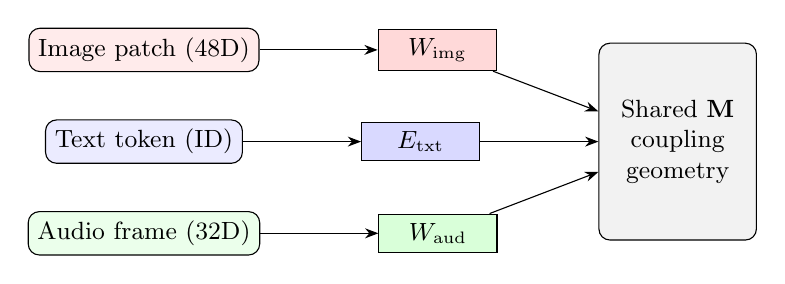
\begin{tikzpicture}[>=Stealth, font=\small, node distance=1.4cm]
    \node[draw, rounded corners, fill=red!8, minimum width=2.5cm] (img) {Image patch (48D)};
    \node[draw, rounded corners, fill=blue!8, minimum width=2.5cm, below=0.6cm of img] (txt) {Text token (ID)};
    \node[draw, rounded corners, fill=green!8, minimum width=2.5cm, below=0.6cm of txt] (aud) {Audio frame (32D)};

    \node[draw, fill=red!15, right=1.5cm of img, minimum width=1.5cm] (pimg) {$W_\text{img}$};
    \node[draw, fill=blue!15, right=1.5cm of txt, minimum width=1.5cm] (ptxt) {$E_\text{txt}$};
    \node[draw, fill=green!15, right=1.5cm of aud, minimum width=1.5cm] (paud) {$W_\text{aud}$};

    \node[draw, rounded corners, fill=gray!10, right=1.5cm of ptxt, minimum width=2cm, minimum height=2.5cm, align=center] (M) {Shared $\M$\\coupling\\geometry};

    \draw[->] (img) -- (pimg);
    \draw[->] (txt) -- (ptxt);
    \draw[->] (aud) -- (paud);
    \draw[->] (pimg) -- (M);
    \draw[->] (ptxt) -- (M);
    \draw[->] (paud) -- (M);
\end{tikzpicture}
\end{center}

Each projection ($W_\text{img} \in \R^{48 \times d}$, $E_\text{txt} \in \R^{V \times d}$, $W_\text{aud} \in \R^{32 \times d}$) is learned independently.
The problem: \textbf{nothing forces these projections to map into the same region of $\R^d$.}

In code, this is what most multimodal models do:

\begin{lstlisting}[caption={Separate projections: each modality gets its own map into $d$-space.}]
class SeparateProjections(nn.Module):
    def __init__(self, d_model, img_dim=48, aud_dim=32, vocab=256):
        super().__init__()
        # Three independent projections -- nothing connects them
        self.img_proj = nn.Linear(img_dim, d_model, bias=False)
        self.aud_proj = nn.Linear(aud_dim, d_model, bias=False)
        self.txt_emb  = nn.Embedding(vocab, d_model)

    def forward(self, data, modality):
        if modality == "image":
            return self.img_proj(data)    # images land HERE in R^d
        elif modality == "audio":
            return self.aud_proj(data)    # audio lands THERE in R^d
        elif modality == "text":
            return self.txt_emb(data)     # text lands ELSEWHERE in R^d
\end{lstlisting}

\paragraph{The failure mode.}
Each \texttt{nn.Linear} initialises with random weights and learns independently during training.
Image projections converge to one region of $\R^d$, text to another, audio to a third.
$\M$'s coupling geometry applies equally to all three regions---but because the regions don't overlap, cross-modal coupling produces near-zero attention weights.

In practice, image patches cluster in one region, text tokens in another, audio frames in a third.
$\M$'s coupling geometry IS shared ($>99.6\%$ similarity across modalities in our experiments), but the modalities never meet---they share the ``road network'' (coupling rules) but have no roads between them.
Cross-modal retrieval: $0\%$.
Zero-shot classification: chance level.

This is the fiber bundle problem from Section~\ref{sec:fiber-bundle}: the base space (coupling geometry) is shared, but the fibers (modality-specific content spaces) are disjoint.

\subsection{The Fix: Shared Projection with Modality Tokens}

The insight from Meta-Transformer~\cite{zhang2023metatransformer}: sharing a \emph{frozen} encoder across 12~modalities works if the tokeniser maps all modalities into a common space.
The coupling geometry is already universal---we just need to get all signals to the same place.

\begin{center}
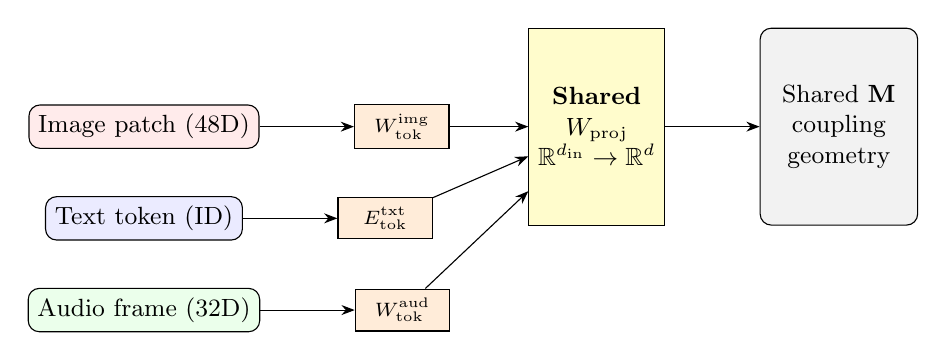
\begin{tikzpicture}[>=Stealth, font=\small, node distance=1.4cm]
    \node[draw, rounded corners, fill=red!8, minimum width=2.5cm] (img) {Image patch (48D)};
    \node[draw, rounded corners, fill=blue!8, minimum width=2.5cm, below=0.6cm of img] (txt) {Text token (ID)};
    \node[draw, rounded corners, fill=green!8, minimum width=2.5cm, below=0.6cm of txt] (aud) {Audio frame (32D)};

    \node[draw, fill=orange!15, right=1.2cm of img, minimum width=1.2cm, font=\scriptsize] (timg) {$W_\text{tok}^\text{img}$};
    \node[draw, fill=orange!15, right=1.2cm of txt, minimum width=1.2cm, font=\scriptsize] (ttxt) {$E_\text{tok}^\text{txt}$};
    \node[draw, fill=orange!15, right=1.2cm of aud, minimum width=1.2cm, font=\scriptsize] (taud) {$W_\text{tok}^\text{aud}$};

    \node[draw, fill=yellow!20, right=1.0cm of timg, minimum width=1.5cm, minimum height=2.5cm, align=center] (shared) {\textbf{Shared}\\$W_\text{proj}$\\$\R^{d_\text{in}} \to \R^d$};

    \node[draw, rounded corners, fill=gray!10, right=1.2cm of shared, minimum width=2cm, minimum height=2.5cm, align=center] (M) {Shared $\M$\\coupling\\geometry};

    \draw[->] (img) -- (timg);
    \draw[->] (txt) -- (ttxt);
    \draw[->] (aud) -- (taud);
    \draw[->] (timg) -- (shared);
    \draw[->] (ttxt) -- (shared);
    \draw[->] (taud) -- (shared);
    \draw[->] (shared) -- (M);
\end{tikzpicture}
\end{center}

The architecture has two stages:
\begin{enumerate}[nosep]
    \item \textbf{Per-modality tokenisers} (small, modality-specific): map raw signals to a common intermediate dimension $d_\text{in}$.
    These are lightweight---a linear layer for image patches, an embedding table for text, a linear layer for audio frames.
    Their job is to normalise scale and dimensionality, not to build rich representations.
    \item \textbf{Shared projection} (one matrix for all modalities): maps $d_\text{in} \to d$.
    Because all modalities go through the \emph{same} linear transform, they are forced into the same region of $\R^d$.
    $\M$ can now couple image-to-text and audio-to-text because they cohabit in the same space.
\end{enumerate}

A learned \textbf{modality token} (\texttt{[IMG]}, \texttt{[TXT]}, \texttt{[AUD]}) is prepended to each sequence.
This gives the model one bit of information---``this sequence is images'' or ``this sequence is text''---without segregating the representations.
The per-layer response heads read the modality token and adapt their processing accordingly.

In code:

\begin{lstlisting}[caption={Shared projection with modality tokens: all modalities enter the same space.}]
class SharedProjection(nn.Module):
    def __init__(self, d_model, img_dim=48, aud_dim=32, vocab=256):
        super().__init__()
        # Stage 1: lightweight per-modality tokenisers
        # (just normalise dimensions -- no heavy lifting)
        input_dim = max(img_dim, aud_dim, d_model)
        self.img_tokenize = nn.Linear(img_dim, input_dim, bias=False)
        self.aud_tokenize = nn.Linear(aud_dim, input_dim, bias=False)
        self.txt_emb      = nn.Embedding(vocab, input_dim)

        # Stage 2: THE KEY -- one shared projection for ALL modalities
        self.shared_proj = nn.Linear(input_dim, d_model, bias=False)

        # Learned modality tokens (one vector per modality)
        self.mod_tokens = nn.ParameterDict({
            "image": nn.Parameter(torch.randn(1, 1, d_model) * 0.02),
            "audio": nn.Parameter(torch.randn(1, 1, d_model) * 0.02),
            "text":  nn.Parameter(torch.randn(1, 1, d_model) * 0.02),
        })

    def forward(self, data, modality):
        # Stage 1: per-modality tokenisation
        if modality == "image":
            h = self.img_tokenize(data)   # (B, S, input_dim)
        elif modality == "audio":
            h = self.aud_tokenize(data)
        elif modality == "text":
            h = self.txt_emb(data)

        # Stage 2: shared projection -- ALL modalities go through
        # the SAME linear transform. This forces them into the
        # same region of R^d, so M can couple them.
        h = self.shared_proj(h)           # (B, S, d_model)

        # Prepend modality token: tells the model "this is images"
        # without segregating the representation space
        B = h.shape[0]
        tok = self.mod_tokens[modality].expand(B, -1, -1)
        h = torch.cat([tok, h], dim=1)    # (B, 1+S, d_model)
        return h
\end{lstlisting}

\paragraph{Line-by-line: what changed and why.}
\begin{itemize}[nosep]
    \item \texttt{img\_tokenize}, \texttt{aud\_tokenize}, \texttt{txt\_emb} --- per-modality, but \emph{small}.
    Their only job is to get each modality to the same intermediate dimension.
    Unlike separate projections, they don't map directly into $\M$'s $d$-space.
    \item \texttt{shared\_proj} --- the critical change.
    One matrix, shared by all modalities.
    Images, audio, and text all pass through the same linear transform.
    Gradients from all modalities flow into this one matrix, forcing it to find a common representation.
    \item \texttt{mod\_tokens} --- a learned vector per modality, prepended to the sequence.
    The model reads this token to know what modality it's processing.
    Unlike separate projections (which encode modality as \emph{geometry}), modality tokens encode it as a \emph{signal}.
    $\M$ can learn to use or ignore this signal as training demands.
\end{itemize}

\paragraph{Why modality tokens, not separate projections?}
Separate projections encode modality identity in the \emph{geometry of the embedding space}---images live ``over there,'' text ``over here.''
A modality token encodes identity as a \emph{signal in the sequence}---all modalities live in the same space, but the model knows which is which from the prepended token.
The difference is fundamental: separate projections make cross-modal coupling geometrically impossible (the spaces don't overlap); modality tokens make it the model's choice (the coupling geometry can link modalities or not, as training requires).

\paragraph{Putting it together with the ORN backbone.}
Here is the complete multimodal V3 forward pass:

\begin{lstlisting}[caption={Multimodal V3: shared projection feeds into shared backbone.}]
class MultimodalORN(nn.Module):
    def __init__(self, d_model, n_layers, n_heads, ffn_width_mult=6):
        super().__init__()
        # Shared input interface (code above)
        self.interface = SharedProjection(d_model)

        # Shared ORN backbone: M + wide FFN
        # (same code as Section 13, but with wide shared FFN)
        self.A = nn.Parameter(torch.randn(d_model, d_model) * 0.02)
        self.B = nn.Parameter(torch.randn(d_model, d_model) * 0.02)
        self.shared_ffn = WideSwiGLU(d_model, d_model * ffn_width_mult)
        self.blocks = nn.ModuleList([
            ORNBlock(d_model, n_heads, self.A, self.B, self.shared_ffn)
            for _ in range(n_layers)
        ])

        # Per-modality output heads
        self.img_head = nn.Linear(d_model, 48, bias=False)
        self.txt_head = nn.Linear(d_model, 256, bias=False)
        self.aud_head = nn.Linear(d_model, 32, bias=False)

    def forward(self, data, modality):
        # Input: raw modality data -> shared d-space
        h = self.interface(data, modality)

        # Backbone: shared M + shared FFN across all layers
        for block in self.blocks:
            h = block(h)

        # Output: modality-specific prediction head
        h = h[:, 1:, :]    # remove modality token
        if modality == "image":
            return self.img_head(h)
        elif modality == "text":
            return self.txt_head(h)
        elif modality == "audio":
            return self.aud_head(h)
\end{lstlisting}

\noindent
The entire backbone---$A$, $B$, \texttt{shared\_ffn}, and the \texttt{ORNBlock} response heads---sees all modalities.
The only modality-specific components are the small tokenisers at the input and the prediction heads at the output.
Everything in between is universal.

\begin{intuition}
\textbf{Realisation: Sub-linear rank growth across modalities (\#48).}
When we train $\M$ on images + audio + text simultaneously, the coupling rank grows sub-linearly.
Three modalities jointly need rank 3---not rank 10 (the sum of individual ranks: 4 + 4 + 2).
That's $3.3\times$ compression.
Music and text are the most compatible pair (rank 4 = max of singles, not sum).
The coupling geometry is partially shared across modalities: the relational rules ``adjacent patches relate spatially'' and ``adjacent words relate syntactically'' activate overlapping eigenmodes of $\M$.
This is why the shared backbone works: modalities share relational structure, not just parameters.
\end{intuition}

\paragraph{What the literature says.}
\begin{itemize}[nosep]
    \item Meta-Transformer~\cite{zhang2023metatransformer}: a frozen encoder trained on images processes 12 modalities with only tokeniser changes.
    The entire attention mechanism transfers---coupling geometry is modality-invariant.
    \item 4M-21~\cite{bachmann2024fourm}: a single transformer handles 21 modalities via modality-specific discrete tokenisers + shared backbone.
    Only modality embeddings and tokenisers are modality-specific.
    \item MoT~\cite{liang2024mot}: shares global self-attention but separates FFN.
    Achieves 55\% FLOP savings.
    ORN V3 tests the opposite---sharing FFN too---to see if a common key-value memory creates cross-modal bridges.
    \item ONE-PEACE~\cite{wang2023onepeace}: shared self-attention + modality adapters at 4B parameters for vision, audio, and language.
\end{itemize}

\subsection{Crystallisation: When Should the Shared Geometry Form?}

A subtlety: if you train all components simultaneously from step~1, the response heads and modality-specific tokenisers can co-adapt, potentially learning shortcuts that bypass $\M$'s coupling geometry.
The result: $\M$ works but doesn't carry universal structure.

A \textbf{crystallisation phase} addresses this:
\begin{enumerate}[nosep]
    \item \textbf{Phase 1 (M-crystallisation):} Alternate between training all parameters (200 steps) and training only $A, B$ (100 steps).
    During $\M$-only steps, the response heads are frozen---$\M$ must discover coupling geometry that works for all modalities without help from modality-specific adaptation.
    \item \textbf{Phase 2 (joint training):} Unfreeze everything and train normally.
    The response heads learn to exploit the crystallised $\M$, but $\M$'s geometry is already established.
\end{enumerate}

This mirrors biological development: neural connectivity (analogous to coupling geometry) forms before functional specialisation.
The result of our frozen-$\M$ experiments ($+0.73\%$ transfer gap at 108M scale) confirms that once crystallised, $\M$'s geometry is reusable---it does not need to be retrained when the downstream task changes.

In code, the crystallisation phase is a training loop modification:

\begin{lstlisting}[caption={M-crystallisation: force M to discover universal geometry before specialisation.}]
def train_with_crystallisation(model, data_loaders, modalities,
                               crystal_steps=2000, total_steps=10000):
    opt = torch.optim.AdamW(model.parameters(), lr=3e-4)

    # ── Phase 1: Crystallise M ──────────────────────────────
    for step in range(crystal_steps):
        modality = modalities[step % len(modalities)]  # round-robin
        x, y = data_loaders[modality].get_batch()

        # Every 3rd step: train ONLY M (freeze everything else)
        if step % 3 == 0:
            for p in model.parameters():
                p.requires_grad = False
            model.A.requires_grad = True   # unfreeze M only
            model.B.requires_grad = True
        else:
            for p in model.parameters():
                p.requires_grad = True     # unfreeze all

        opt.zero_grad()
        _, loss = model(x, modality, targets=y)
        loss.backward()
        opt.step()

    # ── Phase 2: Joint training ─────────────────────────────
    # M is now crystallised. Response heads learn to use it.
    for p in model.parameters():
        p.requires_grad = True

    for step in range(total_steps):
        modality = modalities[step % len(modalities)]
        x, y = data_loaders[modality].get_batch()
        opt.zero_grad()
        _, loss = model(x, modality, targets=y)
        loss.backward()
        opt.step()
\end{lstlisting}

\paragraph{What happens during Phase 1.}
During M-only steps, the response heads cannot adapt.
$\M$ must find a coupling geometry that produces reasonable attention patterns for images, text, and audio \emph{simultaneously}---because it gets no help from modality-specific parameters.
This pressure produces a genuinely universal coupling geometry rather than one that a particular set of response heads has learned to compensate for.

\paragraph{How to check if crystallisation worked.}
After Phase~1, compute $\M$'s effective rank and eigenmode usage per modality:

\begin{lstlisting}[caption={Measuring eigenmode overlap after crystallisation.}]
def measure_eigenmode_sharing(model, data_loaders, modalities):
    A = model.A.detach().cpu()
    B = model.B.detach().cpu()
    M = A @ B.T
    U, S, Vh = torch.linalg.svd(M)  # U columns are eigenmodes

    usage = {}
    for mod in modalities:
        h = get_middle_layer_repr(model, data_loaders[mod])
        # Project onto M's eigenmodes
        energy = (h @ U).pow(2).mean(dim=0)  # energy per mode
        usage[mod] = energy

    # Which of top-20 modes are shared by all modalities?
    top_k = 20
    top_modes = {mod: set(energy.topk(top_k).indices.tolist())
                 for mod, energy in usage.items()}
    shared = set.intersection(*top_modes.values())
    print(f"Shared eigenmodes (top-{top_k}): {len(shared)}/{top_k}")
    # > 10/20 = good, M is universal
    # < 5/20 = M has partitioned by modality
    return shared, usage
\end{lstlisting}

\noindent
If crystallisation works, the shared eigenmode count should be $>50\%$ (the same coupling modes serve all modalities).
If it fails, modes partition by modality---image modes, text modes, audio modes---with little overlap.

\begin{remark}
\textbf{Realisation: The input interface was the failure point, not M (\#197).}
Every prior multimodal experiment showed $>99.6\%$ coupling similarity across modalities---$\M$ was working perfectly.
But cross-modal retrieval was 0\% and zero-shot classification was at chance.
The diagnosis: separate input projections mapped each modality to a different region of $\R^d$.
The modalities shared the road network ($\M$'s coupling rules) but had no roads between them (disjoint fibers).
The shared projection with modality tokens fixes this by ensuring all modalities enter the same region.
Meta-Transformer~\cite{zhang2023metatransformer} proved this works at scale: a frozen encoder transfers to 12 modalities with only tokeniser changes.
\end{remark}

\subsection{Theory-Aligned Multimodal: Three Principles That Made It Work}

Our first multimodal experiment achieved 0\% cross-modal retrieval.
Our second, theory-aligned version reached \textbf{55.6\% cross-modal retrieval} (chance = 10\%) and is still climbing.
The difference came down to three design principles, each derived from the theory that $\M$ must be modality-agnostic.

\paragraph{Principle 1: Single shared CLS token.}
The first version used separate modality tokens (\texttt{txt\_token}, \texttt{img\_token})---different learned starting points for each modality.
This guarantees different orbits regardless of what $\M$ does, because the initial condition determines the trajectory.

The fix: one shared \texttt{cls\_token} for all modalities.
Both text and images start from the same point.
$\M$ processes them through the same coupling geometry.
The modality information comes from the \emph{content} (the tokens/patches after the CLS), not from the starting point.

\begin{verbatim}
  # WRONG: separate starting points → separate orbits
  txt_token = nn.Parameter(torch.randn(1, 1, d))  # text start
  img_token = nn.Parameter(torch.randn(1, 1, d))  # image start

  # RIGHT: shared starting point → orbits can converge
  cls_token = nn.Parameter(torch.randn(1, 1, d))  # same for both
\end{verbatim}

\paragraph{Principle 2: Shared input normalisation.}
Each modality has a different projection (\texttt{txt\_emb}, \texttt{img\_proj}) that maps raw input into $\R^d$.
These projections produce different output distributions---different means, different scales.
$\M$ can trivially distinguish modalities from the input statistics alone, defeating the purpose of shared coupling.

The fix: apply the same \texttt{RMSNorm} after every modality projection, before $\M$ sees the input.
This forces all modalities into the same distribution.
$\M$ cannot tell whether it is processing text or image based on statistics---only the content patterns differ.

\begin{verbatim}
  input_norm = RMSNorm(d)  # shared across all modalities
  h = input_norm(txt_emb(tokens))    # text: normalised
  h = input_norm(img_proj(patches))  # image: same distribution
\end{verbatim}

\paragraph{Principle 3: Paired contrastive from labels.}
The first version used unpaired InfoNCE---pushing random text toward random images.
``A story about a dog'' was pushed toward a random image of a car.
This is noise, not signal.

The fix: create pseudo-captions from class labels (``a picture of a dog'' for CIFAR class 5) and push each image toward its matching caption.
This is the minimum viable pairing---real image-caption data (COCO) would be stronger, but even class-label pseudo-captions provide enough signal to bridge modalities.

\paragraph{Results.}
\begin{center}\small
\begin{tabular}{@{}lrr@{}}
\toprule
Metric & V1 (broken design) & V2 (theory-aligned) \\
\midrule
Cross-modal retrieval & $\approx 0\%$ & \textbf{55.6\% (and climbing)} \\
CIFAR-10 accuracy & 47\% & 60\% \\
\bottomrule
\end{tabular}
\end{center}

The same $\M$, the same wide shared FFN, the same training budget.
The only difference is the three principles above.
The theory works: $\M$ bridges modalities when the input interface is designed to let it.

% ======================================================================
\section{Diffusion and the Semigroup: Native Generative Modelling}
\label{sec:diffusion}
% ======================================================================

The ORN's shared coupling has a deep connection to diffusion models---not as an add-on, but as a native property of the semigroup structure.

\subsection{The Key Insight: $t = \sigma$}

In a standard diffusion model~\cite{song2023consistency}, the denoising process starts from noise ($\sigma = 1$, maximum corruption) and iteratively refines toward data ($\sigma = 0$, clean signal).
At each noise level, the model must learn how to denoise---typically through a U-Net or transformer conditioned on $\sigma$.

In the ORN, the semigroup parameter $t$ scales the coupling strength:
\[
    q = h \cdot (t \cdot A), \quad k = h \cdot (t \cdot B)
\]
At $t = 1$ (full coupling), $\M$ applies its complete relational structure---fine details and coarse structure alike.
At $t = 0.1$ (weak coupling), only the dominant eigenmodes of $\M$ survive---coarse structure only.

\begin{intuition}
\textbf{Realisation: The semigroup coupling $t$ and the diffusion noise $\sigma$ are the same parameter (\#74).}
Setting $t = 1 - \sigma$ means:
\begin{itemize}[nosep]
    \item High noise ($\sigma \to 1$, $t \to 0$): only the strongest eigenmodes of $\M$ contribute to coupling. Coarse structure (topic, genre, spatial layout) is resolved first.
    \item Low noise ($\sigma \to 0$, $t \to 1$): all eigenmodes contribute. Fine detail (specific words, precise pixel values) emerges last.
\end{itemize}
$\M$'s eigenspectrum \emph{is} the noise schedule.
No external schedule needs to be designed---the architecture defines it~\cite{chen2023deeposg}.
Benita et al.\ (2025) prove this formally: the score function decomposes as $\tilde{s}_t(x) = \sum_k \hat{\alpha}_k(t) \nabla \phi_k(x)$, where $\phi_k$ are the semigroup generator's eigenfunctions and $\hat{\alpha}_k(t)$ are $t$-dependent coefficients.
Each eigenmode of $\M$ is an independent denoising channel with its own schedule.
\end{intuition}

\subsection{What We Found Experimentally}

This connection is theoretically beautiful but practically challenging.
We tested three approaches and report honestly:

\paragraph{What failed.}
Native $t$-scaling through coupling (feeding $t$ directly into $A, B$) \textbf{loses} to the simplest baseline (no $t$ conditioning at all) on denoising recovery:

\begin{center}\small
\begin{tabular}{@{}lcc@{}}
\toprule
\textbf{Variant} & \textbf{Recovery@$\sigma{=}0.5$} & \textbf{AR loss} \\
\midrule
A: Native $t$-scaling & 6.6\% & 9.99 \\
B: Fixed $t{=}1$ & 8.4\% & 9.97 \\
C: No conditioning & \textbf{9.6\%} & \textbf{9.27} \\
\bottomrule
\end{tabular}
\end{center}

All three show catastrophic forgetting of the autoregressive (AR) task---loss 9+ when a well-trained model starts at ${\sim}3$.

\paragraph{The diagnosis.}
Two confounds: (1) pure diffusion training destroys the AR capability; (2) the FFN is $t$-unaware, so 75\% of the layer fights the denoising signal.

\paragraph{What worked.}
\textbf{Interleaved training}---alternating AR batches (causal mask, $t{=}1$) with denoising batches (bidirectional, variable $t$)---preserves the AR capability:

\begin{center}\small
\begin{tabular}{@{}lcc@{}}
\toprule
& \textbf{AR loss at step 1000} & \textbf{Denoising} \\
\midrule
Pure diffusion & 9.8 (catastrophic) & learns \\
\textbf{Interleaved 50/50} & \textbf{2.96} (preserved) & learns \\
\bottomrule
\end{tabular}
\end{center}

This confirms the DiffuLLaMA finding~\cite{liu2024llava}: attention mask annealing (gradual causal$\to$bidirectional) prevents forgetting.
The ORN's advantage: $\M$ provides the same coupling geometry in both modes (AR and diffusion), so the interleaving is architecturally natural.

\subsection{The Structural Advantage Conjecture}

Diffusion corrupts \emph{content} but not \emph{structure}.
At any noise level $\sigma$, the rules for how patches relate to patches or how words relate to words are invariant---only the specific content (which pixels, which words) is degraded.
Denoising is the process of recovering content under fixed structural rules.

A standard transformer conflates structure and content.
Each layer has independent $Q, K, V$, FFN---it discovers ``what relates to what'' and ``what the answer is'' simultaneously, in the same parameters.
When you corrupt the input, it must untangle both from noisy data.

A shared $\M$ separates them architecturally.
$\M$ provides the structural rules once (which tokens should couple).
The noise level $t$ modulates which modes of that structure are visible.
The denoiser's job simplifies from ``figure out structure AND content'' to just ``figure out content under the structure $\M$ provides.''

\begin{remark}
\textbf{This is not yet proven.}
The structural advantage conjecture is the strongest theoretical argument for the ORN over the transformer---not parameter savings, not scaling curves, but that the architecture's structure matches the task structure for diffusion.
However, the native $t$-scaling experiment failed, and the interleaved training fix has not yet been run to completion with proper $t$-conditioning (adaLN).
The conjecture remains a prediction to be tested, not a confirmed result.
What would falsify it: a standard transformer with the same interleaved training recipe matching or beating the ORN on diffusion metrics.
\end{remark}

\subsection{The Four Inference Modes}

If the diffusion connection holds, one ORN supports four inference modes from the same weights:

\begin{description}[nosep]
\item[1. Autoregressive:] $t{=}1$, causal mask. Standard next-token prediction. Fast.
\item[2. Diffusion:] Variable $t$ schedule (high$\to$low), bidirectional mask. Iterative refinement from noise. Higher quality, slower.
\item[3. Infilling:] Mask middle of sequence, denoise with bidirectional attention. The killer app for editing.
\item[4. Brainstorming:] Multiple diffusion trajectories from the same noise. $\M$'s eigenmodes define the space of ``plausible alternatives.''
\end{description}

No architectural changes between modes---only the mask and $t$ schedule change.
This is because $\M$'s coupling geometry is the same object whether you read it autoregressively or iteratively.

\begin{lstlisting}[caption={Four modes from one model: only mask and $t$ change.}]
def generate_ar(model, prompt_ids, max_new=100):
    """Mode 1: autoregressive. t=1, causal mask."""
    return model.generate(prompt_ids, max_new=max_new)

def generate_diffusion(model, seq_len, steps=20):
    """Mode 2: diffusion. t schedule high->low, bidirectional."""
    tokens = torch.randint(0, vocab, (1, seq_len))
    for step in range(steps):
        t = 1.0 - step / steps  # coupling strength: weak -> full
        sigma = 1.0 - t         # noise level: high -> low
        logits = model(tokens, t=t, is_causal=False)
        # Replace low-confidence tokens with model predictions
        probs = logits.softmax(-1)
        confidence = probs.max(-1).values
        threshold = confidence.quantile(1 - (step+1)/steps)
        replace = confidence >= threshold
        tokens[0, replace] = probs[0, replace].argmax(-1)
    return tokens

def infill(model, tokens, mask_positions, steps=10):
    """Mode 3: infilling. Mask specified positions, denoise."""
    for step in range(steps):
        t = (step + 1) / steps
        tokens[:, mask_positions] = torch.randint(0, vocab, ...)
        logits = model(tokens, t=t, is_causal=False)
        tokens[:, mask_positions] = logits[:, mask_positions].argmax(-1)
    return tokens
\end{lstlisting}

% ======================================================================
% ======================================================================
\section{Spectral Embeddings: Mode-Selective Retrieval}
\label{sec:spectral-embed}
% ======================================================================

$\M$'s eigenspectrum provides a natural decomposition of the embedding space into functionally distinct bands.
This section explains the idea, the experimental evidence, and how to build a mode-selective retrieval system.

\subsection{The Key Idea: Different Eigenmodes Encode Different Things}

Compute the SVD of $\M = AB^\top$: the singular values tell you \emph{how much energy} each mode carries, and the singular vectors tell you \emph{which directions} in $\R^d$ they correspond to.

A representation vector $v$ can be projected onto any subset of these modes:
\begin{align}
    v_{\text{top}} &= V_h[{:}k]^\top \cdot v \quad\text{(top $k$ modes --- communicative form)} \\
    v_{\text{tail}} &= V_h[m{:}]^\top \cdot v \quad\text{(tail modes --- topic/content)}
\end{align}
where $V_h$ are $\M$'s right singular vectors.

\paragraph{What we found empirically.}
Probing 14 text properties across 9 spectral bands (V2 108M, 500 TinyStories texts):
\begin{itemize}[nosep]
    \item \textbf{Top 5 modes:} strongest signal is \texttt{has\_question} (silhouette 0.083).  The very top of the eigenspectrum distinguishes questions from statements.
    \item \textbf{Top 13 modes:} \texttt{has\_dialog} (0.053) and \texttt{has\_names} (0.044).  Dialog and named-character presence.
    \item \textbf{Tail modes:} topic/content signal is strongest here, though not cleanly separated on TinyStories.
\end{itemize}

The top modes encode \emph{communicative form}---what kind of text is this (question, dialog, narration)?
The tail modes carry \emph{content}---what is the text about (animals, food, weather)?

This is not arbitrary: $\M$'s dominant eigenmodes define the strongest coupling patterns, which are structural (interrogative syntax, dialog turn-taking, coreference).
Content-specific patterns (word choice, entity identity) are weaker couplings that live in the tail.

\subsection{ORN vs GPT-2: Does SharedM Help?}

We compared ORN V2 (108M, explicit shared $\M$) against GPT-2 Small (124M, with averaged $W_Q W_K^\top$ as effective $\M$) on a balanced corpus (225 texts, 3 forms $\times$ 3 topics):

\begin{center}\small
\begin{tabular}{@{}lrr@{}}
\toprule
Band & Topic kNN & Topic Silhouette \\
\midrule
ORN Tail 70+ & \textbf{79.1\%} & \textbf{+0.117} \\
GPT-2 Tail 93+ & 64.0\% & +0.016 \\
GPT-2 Top 17 & 35.1\% & $-$0.063 \\
\bottomrule
\end{tabular}
\end{center}

ORN tail modes achieve 79.1\% topic accuracy (chance = 33\%) with positive silhouette.
GPT-2 top modes are \emph{anti-topic} (35\%, negative silhouette)---the averaged M captures form but destroys content geometry.
SharedM produces a spectral decomposition where the fiber is real and clustered; the averaged coupling matrix does not.

\subsection{Building a Mode-Selective RAG System}

The key mechanism is \textbf{projection onto eigenmode bands}.
$\M$'s SVD gives right singular vectors $V_h$---these define the eigenbasis.
Projecting any representation onto a subset of modes is a single matrix multiply:

\begin{verbatim}
  # Compute M's SVD once (shared, fixed after training)
  _, S, Vh = torch.linalg.svd(model.A @ model.B.T)

  # Embed a text: forward through ORN, mean-pool
  v = orn_forward(text).mean(dim=1)    # shape: (d,)

  # Project onto form modes (top 13 of M's eigenbasis)
  v_form  = normalize(v @ Vh[:13].T)   # shape: (13,)

  # Project onto topic modes (tail, modes 70+)
  v_topic = normalize(v @ Vh[70:].T)   # shape: (506,)
\end{verbatim}

The same projection applies to both documents (at index time) and queries (at search time).
FAISS stores one index per mode; at query time, you choose which index to search:

\begin{enumerate}[nosep]
    \item \textbf{Index time:} For each document, compute the ORN embedding, project onto each band, add to the corresponding FAISS index.
    \item \textbf{Query time:} Compute the query embedding, project onto the desired band, search the matching FAISS index.
    \item \textbf{Mode selection:}
    \begin{itemize}[nosep]
        \item ``Find documents with the same structure'' $\to$ form index (13 dimensions).
        \item ``Find documents about the same topic'' $\to$ topic index (506 dimensions).
        \item ``Find the most similar overall'' $\to$ full index (576 dimensions).
    \end{itemize}
    \item \textbf{Cascade} for efficiency: topic filter (fast, 506d) $\to$ full rerank (precise, 576d).
\end{enumerate}

The projection costs one matrix multiply per query---negligible compared to the ORN forward pass.
The topic index achieves 77.8\% nearest-neighbour accuracy while using 88\% fewer dimensions than the full embedding.

% ======================================================================
\section{Metaphors We Live By: Why \texorpdfstring{$\M$}{M} Captures Conceptual Structure}
\label{sec:metaphors}
% ======================================================================

This section connects the ORN's spectral decomposition to one of the most influential theories in cognitive linguistics.

\subsection{The Theory: Conceptual Metaphor}

In 1980, George Lakoff and Mark Johnson published \emph{Metaphors We Live By}~\cite{lakoff1980}, arguing that abstract thought is not literal---it is structured by \textbf{metaphor}.
Not poetic metaphor, but \emph{conceptual metaphor}: systematic mappings that organise how we think.

Consider: ``\textbf{Argument is war}.''
\begin{itemize}[nosep]
    \item ``He \emph{attacked} my position.''
    \item ``She \emph{defended} her claim.''
    \item ``His argument was \emph{indefensible}.''
    \item ``I \emph{won} the debate.''
\end{itemize}

This is not decoration---it is how English speakers structure the concept of argument.
The relational pattern (agents opposing each other, using strategies, achieving outcomes) is \emph{borrowed from war} and applied to intellectual exchange.

Lakoff identified dozens of these: \textsc{time is money} (we \emph{spend}, \emph{save}, \emph{waste} time), \textsc{ideas are food} (I can't \emph{digest} that, a \emph{half-baked} idea), \textsc{understanding is seeing} (I \emph{see} what you mean, a \emph{clear} explanation).

The key insight: in every case, the \textbf{relational structure} is preserved while the \textbf{content} changes.

\subsection{The Connection to the ORN}

This is exactly what $\M$'s eigenspectrum does.

\paragraph{Top modes = relational structure (the metaphor).}
$\M$'s top eigenmodes encode what-couples-to-what: agent-action-object, cause-effect, container-contents.
These patterns are the same whether the sentence is about war or argument, about money or time.

\paragraph{Tail modes = domain content (the specific topic).}
The tail modes encode which words, which entities, which domain.
``Attacked a position'' vs ``attacked a fortress''---same top modes, different tail modes.

\paragraph{Metaphor = orbit equivalence.}
Two sentences that are metaphorically related (``she defended her thesis'' and ``the troops defended the city'') should traverse $\M$'s eigenspectrum identically---same coupling pattern at each layer---while differing in tail-mode content.

We measured this: orbit trajectories achieve 97.7\% communicative form classification, and top modes \emph{anti-cluster} by topic (silhouette $-0.072$).
The structural skeleton is genuinely independent of content.

\subsection{Image Schemas: The Atoms of Thought}

Lakoff went further: all conceptual metaphors ultimately ground in \textbf{image schemas}---simple spatial/bodily patterns learned from physical experience as infants:

\begin{center}\small
\begin{tabular}{@{}lll@{}}
\toprule
Schema & Physical & Abstract extension \\
\midrule
Containment & ``the ball is \emph{in} the box'' & ``the idea is \emph{in} the paper'' \\
Path & ``she walked \emph{to} the park'' & ``the project moved \emph{to} completion'' \\
Force & ``he \emph{pushed} the door'' & ``she \emph{pushed} the argument'' \\
Balance & ``the scale \emph{tipped}'' & ``the evidence \emph{tipped} the case'' \\
Link & ``the rope \emph{connects} them'' & ``friendship \emph{connects} them'' \\
\bottomrule
\end{tabular}
\end{center}

If $\M$ encodes these schemas in its top eigenmodes, then the spectral decomposition is not an arbitrary compression---it is a computational implementation of how human cognition structures abstract thought.

\subsection{What This Predicts}

\begin{enumerate}[nosep]
    \item \textbf{Same schema, different domain $\to$ same top modes.}
    ``The cat is in the box,'' ``the flaw is in the argument,'' and ``she is in a good mood'' should activate the same top eigenmodes of $\M$.
    Domain differences (physical vs logical vs emotional) should appear only in the tail.

    \item \textbf{Different schema, same domain $\to$ different top modes.}
    ``The idea is \emph{in} the paper'' (containment) vs ``the idea \emph{led to} a breakthrough'' (path) should activate different top modes even though both are about ideas.

    \item \textbf{Metaphor composition = eigenmode composition.}
    \textsc{time is money} + \textsc{money is a resource} $\to$ \textsc{time is a resource}.
    Composing two metaphors should correspond to composing two eigenmode activation patterns.
\end{enumerate}

\subsection{Experimental Result: Schemas Found in \texorpdfstring{$\M$}{M}}

We tested predictions 1 and 2 on the V2 108M checkpoint (4B tokens, FineWeb-Edu).
Four schemas (containment, path, force, scale) $\times$ 4 sentences each across physical/social/abstract domains.

\paragraph{The design lesson.}
Mean-pooling over the sentence gave silhouette +0.055---barely above noise.
The fix: extract $\M$'s eigenmode activation at the \textbf{specific token} carrying the schema (``in'' for containment, ``pushed'' for force).
The schema signal is per-token, not per-sentence.

\paragraph{Result: top 5 modes cluster by schema at +0.470 silhouette.}
Top modes beat tail modes (+0.389) and full representation (+0.395).
The force schema clusters tightest: ``pushed the door'' and ``pushed the team'' have 0.935 cosine similarity in $\M$'s top eigenmodes---nearly identical coupling structure across physical and social domains.
Between-schema similarity is lower (0.28--0.66), confirming different schemas occupy different regions of $\M$'s top eigenspace.

$\M$ has discovered image schemas from next-token prediction alone.

\subsection{Why This Matters for Embeddings and Retrieval}

Mode-selective retrieval (Section~\ref{sec:spectral-embed}) becomes \textbf{metaphor-aware retrieval}:

\begin{itemize}[nosep]
    \item \textbf{Top-mode search}: ``find documents with the same relational structure'' = find documents using the same conceptual metaphor.
    A query about military strategy retrieves documents about business competition, legal battles, and chess---all sharing the \textsc{conflict} schema.
    \item \textbf{Tail-mode search}: ``find documents about the same topic'' = find documents in the same domain, regardless of metaphorical framing.
    \item \textbf{Combined}: standard retrieval.
\end{itemize}

No other architecture provides this decomposition, because no other architecture has a shared coupling operator whose eigenspectrum separates relational structure from domain content.

% ======================================================================
\section{Why Contrastive Training Is Essential, Not Optional}
\label{sec:contrastive}
% ======================================================================

This is one of the most important lessons from the ORN embedding experiments.

\subsection{Two Kinds of Coupling}

$\M$ trained with next-token prediction learns \textbf{within-sequence coupling}: which tokens should attend to which inside a single text.
This is local---it says nothing about how different texts, images, or documents relate to each other.

\textbf{Between-sequence coupling}---``these two texts are about the same thing,'' ``this image matches this caption''---requires a different training signal.
Contrastive loss provides it: push matching pairs together, push non-matching pairs apart.

\begin{center}\small
\begin{tabular}{@{}lll@{}}
\toprule
Training signal & What it teaches $\M$ & What it enables \\
\midrule
Next-token prediction & Within-sequence coupling & Language modelling, generation \\
Contrastive loss & Between-sequence coupling & Retrieval, similarity, alignment \\
\bottomrule
\end{tabular}
\end{center}

Without contrastive training, ORN V2 (108M, FineWeb-Edu) scores 0.31 on STSBenchmark---below GloVe (0.58).
The model predicts the next word well but cannot judge whether two sentences mean the same thing.
With even 100 steps of SimCSE (unsupervised contrastive), retrieval improves.

\subsection{Why This Matters for Multimodal}

The ``fiber disjointness problem'' from multimodal experiments is a direct consequence of missing between-sequence signal.
$\M$ discovers that images and text couple with $>$99.6\% similarity---the same structural rules apply.
But the modalities land in different regions of $\R^d$.
$\M$ never received a signal that a picture of a dog and the word ``dog'' should be \emph{near each other}.

Contrastive loss builds the \textbf{on-ramps} between modalities.
This is not a post-hoc fix---it is a fundamental training signal that $\M$ needs to organise global structure.

\subsection{Implication for ORN Training}

Standard practice: train the LM first, fine-tune for embeddings later.

Better for ORN: \textbf{interleave next-token and contrastive from step 1}.
Both signals shape $\M$'s eigenspectrum:
\begin{itemize}[nosep]
    \item Next-token crystallises local coupling geometry (top eigenmodes encode communicative form)
    \item Contrastive crystallises global sequence organisation (tail eigenmodes should cluster by topic/content)
\end{itemize}

A bonus: $\M$'s spectral decomposition provides \textbf{free hard negatives} for contrastive training.
Two texts close in top modes (same form) but far in tail modes (different topic) are natural hard negatives.
No external model needed---the geometry provides them.

% ======================================================================
\section{Where to Go From Here}
\label{sec:future}

\subsection{The Two-System Architecture}

Not all knowledge is structural.
``Caesar crossed the Rubicon in 49~BC'' is a \emph{fact}---it cannot be derived from structure alone.
Orbital embeddings are good at structural knowledge (roles, relationships, categories) but cannot compress arbitrary facts.
This distinction has deep roots in neuroscience: McClelland et al.~\cite{mcclelland1995} showed that the brain uses complementary learning systems---fast hippocampal memory for specific episodes and slow neocortical learning for structural regularities.
LeCun's JEPA~\cite{lecun2022} and Ha \& Schmidhuber's World Models~\cite{ha2018} argue that AI should learn compact generators of dynamics, not catalogues of states.

The proposed solution is a \textbf{two-system architecture}:
\begin{enumerate}[nosep]
    \item \textbf{Orbital world model}: shared dynamics $\Phi$ for structural knowledge.
    Cheap, compressed, generalises.
    \item \textbf{Sparse lookup layer}: a small, separately trained table for factual knowledge.
    Expensive per token, but only needed for fact-bearing tokens.
\end{enumerate}

\begin{figure}[h]
\centering
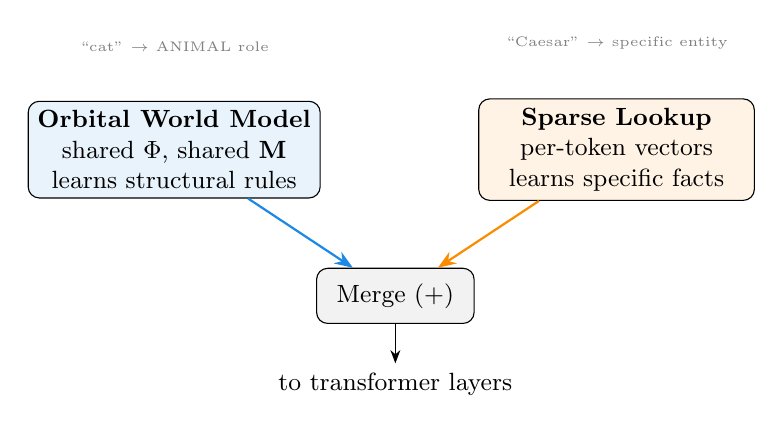
\begin{tikzpicture}[>=Stealth, node distance=1.5cm, font=\small]
    \node[draw, rounded corners, fill=orbitblue!10, minimum width=3.5cm, minimum height=1cm, align=center] (orbit) {\textbf{Orbital World Model}\\shared $\Phi$, shared $\M$\\learns structural rules};

    \node[draw, rounded corners, fill=dynamicsorange!10, minimum width=3.5cm, minimum height=1cm, align=center, right=2cm of orbit] (lookup) {\textbf{Sparse Lookup}\\per-token vectors\\learns specific facts};

    \node[draw, rounded corners, fill=gray!10, minimum width=2cm, minimum height=0.7cm, below=1.5cm of $(orbit)!0.5!(lookup)$] (merge) {Merge ($+$)};

    \draw[->, thick, orbitblue] (orbit) -- (merge);
    \draw[->, thick, dynamicsorange] (lookup) -- (merge);

    \node[above=0.5cm of orbit, font=\tiny, gray] {``cat'' $\to$ ANIMAL role};
    \node[above=0.5cm of lookup, font=\tiny, gray] {``Caesar'' $\to$ specific entity};

    \node[below=0.5cm of merge] (out) {to transformer layers};
    \draw[->] (merge) -- (out);
\end{tikzpicture}
\caption{\textbf{Two-system architecture.}
The orbital system handles structural knowledge (cheap, shared dynamics).
The sparse lookup handles factual knowledge (expensive, per-token storage).
The two are merged before entering the transformer backbone.
This mirrors the cortex--hippocampus division in biological memory.}
\label{fig:two-system}
\end{figure}

\paragraph{Practical implications: adaptation, modularity, and parallelism.}
The two-system split has consequences beyond compression.

\textbf{Adaptation without retraining the world model.}
If the orbital core captures structural knowledge and the ontological layer captures domain-specific bindings, then adapting the model to a new domain---new terminology, new entities, new facts---can be done by swapping or fine-tuning the ontological layer alone, leaving the orbital world model frozen.
This is the natural architecture for retrieval-augmented generation (RAG): the retrieval system populates the ontological layer with context-specific bindings, while the orbital core provides the structural reasoning that makes sense of them.
Fine-tuning becomes surgery on the sparse, cheap component rather than gradient descent through the entire model.
The ontological layer is, in effect, an \emph{in-context fine-tuning surface}.

\textbf{Mixture of experts and the shared residual.}
In a standard transformer, mixture-of-experts (MoE) architectures must route tokens to specialised FFN experts, but those experts communicate only indirectly through the residual stream---a stream whose geometry is shaped by dense, per-layer projections with no explicit shared structure.
When the residual field has a shared geometric structure (our $\M$), expert outputs live in a \emph{common geometric space} with well-defined distances, directions, and coupling rules.
Experts don't just write vectors into a residual stream; they write perturbations into a shared manifold whose geometry is known to the coupling mechanism.
This gives MoE a more natural communication substrate: the shared metric defines what ``nearby'' means, so expert outputs compose coherently even when produced by different specialists.

\textbf{Parallelisation.}
The same argument applies to parallelism more broadly.
When processing is distributed across devices, the shared geometry provides a \emph{coordination-free protocol}: each device knows the manifold structure via $\M$, so partial results can be merged without explicit synchronisation of coupling rules.
The shared residual field acts as a social medium---agents (layers, experts, devices) contribute to a common geometric space whose structure is agreed upon in advance, not negotiated per interaction.

\subsection{The Ontological Layer: Design, Constraints, and the Training Problem}
\label{sec:onto-design}

The two-system idea sounds clean in theory.
In practice, the ontological layer is the hardest part of the architecture to get right.

\paragraph{Design 1: Static per-token correction (too simple).}
The simplest approach: a small per-token embedding $u_w \in \R^{r}$ (rank $r \ll d$), projected to $d_{\text{model}}$ and added to the value stream at every layer.

\begin{lstlisting}[caption={Static ontological correction (Exp 4b)}]
# Per-token code: V x r_onto embedding
onto = onto_proj(onto_emb(token_ids))  # (B, S, d_model)

# In each GRF block:
q = h @ A              # coupling from orbital stream only
k = h @ B              # coupling from orbital stream only
v_input = h + onto     # value = orbital + ontological
v = Wv(v_input)        # response extracts from augmented stream
\end{lstlisting}

\noindent
The constraint is on line 5: the coupling ($q$, $k$) sees only the orbital stream $h$.
The ontological signal enters through the \emph{value} path only.
$\M$ determines \emph{who talks to whom} (structural); $u_w$ determines \emph{what they say} (specific).

The problem: this gives ``Lily'' the \textbf{same correction vector in every context}.
``Lily wanted cake'' and ``Lily was happy'' both get the same $u_{\text{Lily}}$.
But the identity information ``this is Lily'' needs to interact with context---``Lily who wants'' contributes differently from ``Lily who is happy.''
A static per-token vector cannot do contextual binding.

Our Exp~4b tested this design.
Result: the ontological contribution gap was $-1.7\%$---nearly zero.
The static correction did not learn to contribute meaningfully.

\paragraph{Design 2: Contextual ontological adapter (the right idea).}
The ontological layer needs its own attention mechanism to \emph{bind identity into context}.
Our Exp~4 design:

\begin{lstlisting}[caption={Contextual ontological adapter (Exp 4)}]
class OntologicalAdapter(nn.Module):
    def __init__(self, d_model, d_adapter, n_layers=2):
        self.proj_in = Linear(d_model, d_adapter)   # compress
        self.blocks = [                              # tiny attention
            SelfAttention(d_adapter) + FFN(d_adapter)
            for _ in range(n_layers)
        ]
        self.proj_out = Linear(d_adapter, d_model)   # expand

    def forward(self, orbit_hidden):
        h = self.proj_in(orbit_hidden)   # project to adapter space
        for block in self.blocks:
            h = block(h)                  # contextual processing
        return self.proj_out(h)           # correction in d_model space
\end{lstlisting}

\noindent
This adapter \emph{reads} the orbital hidden states (the structural context), processes them through its own small attention (contextual binding), and outputs a correction.
It runs \textbf{after} the orbital engine, on the frozen orbital representations.

\paragraph{The deeper question: whose coupling should the ontological layer use?}

There are three options:
\begin{enumerate}[nosep]
    \item \textbf{Its own learned $Q, K$} (Exp~4's design).
    The adapter learns its own coupling rule for identity binding.
    Maximally flexible, but expensive and may not share structural routing.

    \item \textbf{The shared $\M$} (not yet tested).
    Use $\M$ for coupling (the structural routing is correct---CHARs attend to ACTIONs),
    but feed identity-enriched values through it.
    This is the most principled design: $\M$ determines \emph{routing}, the ontological
    content determines \emph{what flows through that routing}.
    Cheap (no new coupling params), and forces the ontological layer to ride the
    orbital geometry rather than competing with it.

    \item \textbf{No attention} (Exp~4b's static design).
    Just a per-token vector.
    Too simple---cannot do contextual binding.
\end{enumerate}

Option 2 was our initial guess.
However, Exp~7 showed that even the cheaper dual-pathway design (Design~C in the lab notebook) underperforms at 10M: the parallel ontological attention consumes parameter budget without contributing proportionally.

\paragraph{The current best idea: perturbative corrections.}
Rather than a separate attention pathway, the ontological correction is a \emph{small, context-gated perturbation} applied after each SharedM layer:
\[
    \x = \x_{\text{orbital}} + g(\x) \cdot \delta(\x)
\]
where $g$ is a learned gate that reads the residual stream and $\delta$ is a small correction MLP.

\paragraph{How the gate works.}
The gate is mechanically simple: $g = \sigma(W_g \x + b_g)$, a single linear projection through sigmoid.
But what it \emph{reads} is rich.
By layer~$\ell$, the residual stream $\x^{(\ell)}$ contains everything computed so far: the token's identity (from the embedding), its positional encoding, what other tokens it has attended to (from $\M$'s coupling at layers $1$ to $\ell{-}1$), and the functional role the orbit has assigned it.
The gate learns a direction in this space that corresponds to ``enough context has accumulated to warrant a correction.''

This makes the gate a form of \textbf{in-context learning}: it does not fire based on the token identity (that would be a per-token lookup), but based on the \emph{state of the residual stream}, which depends on the full context window.
The same token receives different gate values in different contexts, because the residual stream carries different contextual information.

The gate bias is initialised at $-3$ (so $\sigma(-3) \approx 0.05$---nearly closed).
The perturbation must be \emph{learned to be useful}; it does not contribute by default.
A testable prediction: the gate magnitude should \textbf{negatively correlate with attention entropy}.
When attention is diffuse (high entropy, uncertain coupling), there is no clear context signal to correct with---the gate should stay closed.
When attention is sharp (low entropy, confident coupling), the model knows what is relevant and can make a specific correction---the gate should open.
Exp~8 measures this correlation.

\begin{remark}
\textbf{Realisation: Corrections are essential, not optional (\#28).}
Ablating the corrections (setting $g{=}0$ at inference) increases val loss by \textbf{0.449 nats}---larger than the entire training improvement from step 1,000 to step 5,000 for SharedM alone.
The gate-entropy anticorrelation is $r = -0.95$: the corrections activate precisely when attention coupling is sharp and context is rich.
Gate dynamics confirm the ``dormant early, active late'' prediction: opens from 0.05 (step~1) to 0.36 (step~4,000).
Late sequence positions benefit more ($+0.440$ nats) than early ($+0.392$), confirming context-dependence.
At V2 scale (108M), correction gates are active at 0.29--0.40 across all 24 layers, with layer~8 (the structural-to-content transition) showing the highest gate activity.
The corrections are not a minor refinement---they carry substantial prediction work that the shared coupling geometry cannot provide alone.
\end{remark}

The additive structure $\x = \x_{\text{orbital}} + g \cdot \delta$ is natural because the residual stream is already a space where additive contributions accumulate---every transformer layer adds $\text{attn}(\x) + \text{ffn}(\x)$ to the same stream.
In principle, multiple independent corrections can be composed: $\x = \x_{\text{orbital}} + g_1 \delta_1 + g_2 \delta_2 + \cdots$, each addressing a different aspect (context, entity, style), each independently gated.
This opens a modular fine-tuning surface: freeze the orbital core, add correction terms for new domains or tasks.

\paragraph{The training schedule problem.}
Even with the right architecture, training is hard because of a chicken-and-egg:

\begin{itemize}[nosep]
    \item The orbital system needs to learn $\M$ (the structural coupling) before the ontological
          layer can meaningfully contribute.
          If the ontological layer is active from step 0, it may prevent $\M$ from developing
          by capturing all useful signal in the per-token corrections.
    \item But if the ontological layer starts too late, it may never catch up---the orbital
          system has already found a (suboptimal) way to encode identity information,
          and the ontological layer has nothing to correct.
\end{itemize}

\noindent
The Exp~4 design addresses this by \textbf{phasing}: train the orbital engine first (on anonymised data), freeze it, then train the adapter.
This guarantees the orbital system learns pure structure.

Joint training (Exp~4b) is harder.
Possible solutions:
\begin{itemize}[nosep]
    \item \textbf{Capacity constraint:} make the ontological layer very small (rank $r = 2$--$4$) so it physically cannot capture everything.
    \item \textbf{Annealing:} start with ontological contribution $\lambda = 0$, gradually increase.
    \item \textbf{Gradient scaling:} multiply ontological gradients by a small factor early in training.
    \item \textbf{Regularisation:} L1 penalty on ontological norms, encouraging sparsity.
\end{itemize}

\paragraph{The ontological layer MUST be constrained.}
This is non-negotiable.
Without a hard capacity constraint, the ontological layer will eat everything.
Given $V \times r$ parameters and $r$ anywhere close to $d$, gradient descent will find it easier to dump all information into the per-token ontological codes than to learn a shared dynamical law.
The result: the orbital system goes unused, $\M$ collapses to noise, and you have rebuilt a lookup table with extra steps.

The constraint can be architectural (rank $r \ll d$, sparsity, or value-only injection) or it can be a regularisation penalty.
But it must be there.
The ontological layer is not an optional enhancement---it is a \textbf{deliberately impoverished} system forced to handle only what the orbital system cannot.

\paragraph{Two roles, two phases.}
The ontological layer serves different purposes at different stages:

\textbf{During training: bootstrapper.}
At initialisation, the orbital system has learned nothing---$\M$ is random, the residual stream carries no useful structure.
The ontological layer can provide early gradient signal by doing simple per-token prediction (like a small lookup table).
As the orbital system matures and $\M$ develops structural coupling, the ontological layer's contribution should naturally decline---the orbital system handles more and more of the prediction.
This is the \emph{scaffolding} that gets removed as the building takes shape.

\textbf{After training: fine-tuning surface.}
Once the orbital core is trained, the ontological layer becomes an \emph{adaptation interface}.
To deploy the model in a new domain (new terminology, new entities, new facts), freeze the orbital core and fine-tune only the ontological layer.
This is cheap (the ontological layer is small) and targeted (only the domain-specific bindings change; the structural reasoning is preserved).
The ontological layer is, in effect, an \textbf{in-context fine-tuning surface}---the place where you plug in new knowledge without touching the world model.

This dual role---bootstrapper during training, adaptation surface after---is what makes the constraint essential.
If the ontological layer were large enough to capture everything, there would be nothing to fine-tune (it would already contain the full model) and nothing for the orbital system to learn (the ontological layer would have done the work).
The constraint forces the split: orbital learns the reusable structure; ontological provides the disposable details.

\bigskip
\noindent
This is the most open part of the research programme.
The architectural design is clear; the training protocol is not.
Our current experiments (Exp~4b running, Exp~4 queued) test the two ends of the spectrum: joint training with a static layer vs.\ phased training with a contextual adapter.

\subsection{Scaling Predictions}

The compression advantage of orbital embeddings \emph{grows} with vocabulary size and model dimension:
\begin{itemize}[nosep]
    \item Lookup scales as $\bigO(V \times d)$---linear in both.
    \item Orbital scales as $\bigO(V \times d_s + d^2)$---linear in $V$ but with much smaller coefficient, and the shared dynamics cost is independent of $V$.
\end{itemize}
At $V = 100$K and $d = 4096$ (LLaMA-scale), the lookup table would be 400M parameters.
Orbital at $d_s = 16$ would be 1.6M + 40M = 41.6M---a $\mathbf{10\times}$ compression.

\paragraph{$d_{\text{seed}}$ is a property of the vocabulary, not the model.}
The seed dimension depends on the intrinsic structure of the vocabulary---how many independent functional roles and distributional patterns exist.
Our CPU tests measured this: 90\% of variance in 27 dimensions for structured embeddings.
This does not change when the model grows from 10M to 200M parameters---the vocabulary is the same 50K tokens.

This means $d_{\text{seed}} = 32$ should work at any scale.
What changes is the compression ratio:

\begin{center}\small
\begin{tabular}{@{}lccc@{}}
\toprule
\textbf{Scale} & \textbf{Lookup \% of model} & \textbf{$d_{\text{seed}}{=}32$ \% of model} & \textbf{Compression} \\
\midrule
10M  & 88\% & 16\% & $5.5\times$ \\
50M  & 39\% & 3\%  & $12\times$  \\
200M & 19\% & 1\%  & $24\times$  \\
\bottomrule
\end{tabular}
\end{center}

At 200M parameters, the seeds cost 1.6M---less than 1\% of the model.
The compression ratio \emph{grows} with scale because the lookup table grows as $V \times d$ while the seeds stay at $V \times d_{\text{seed}}$.
Orbital embeddings get more attractive at larger scale, not less---\emph{in theory}.
In practice, even at LLaMA scale, the embedding table is $<$10\% of total parameters and is accessed with zero compute (a single gather operation).
The orbital alternative requires iterating $\Phi$ for every token, adding compute where there was none.
Until vocabularies grow to 500K+ (multilingual, code, multimodal token spaces) or until the seed interpolation property is needed for unseen tokens, standard tied embeddings remain the practical choice.
The V2 and V3 models that beat GPT-2 use standard tied embeddings.

\subsection{Connection to the Broader ORN Programme}

Orbital embeddings are one piece---and currently the least practical piece---of a larger architecture:
\begin{description}
    \item[Orbital embeddings:] Replace the embedding table. Seeds + shared dynamics.
    \item[Shared coupling $\M$:] Replace per-layer $W_Q, W_K$. One metric tensor, shared across layers. \textbf{Validated}: 108M model beats GPT-2 on 5/8 benchmarks with $48\times$ fewer coupling parameters. Frozen $\M$ transfers at $+0.73\%$.
    \item[Shared wide FFN (V3):] Replace $L$ per-layer FFNs with one $L\times$-wider shared FFN~\cite{onewideffn2023, geva2021ffn}. \textbf{Validated at small scale}: $-0.8\%$ vs per-layer at matched params. Currently training at 61M on 50B tokens.
    \item[Per-layer response heads:] $W_V, W_O$ remain per-layer---they encode how each layer \emph{responds} to the shared coupling. These are the \emph{only} component that must vary with depth.
\end{description}
The principle is the same throughout: if a computation is approximately the same across instances (tokens, layers), share the parameters and iterate.
Orbital embeddings illustrate this principle pedagogically; shared coupling and shared FFN deliver it in practice.

\subsection{Open Questions}

\begin{itemize}[nosep]
    \item \textbf{Optimal $d_{\text{seed}}$}: Our CPU tests show 90\% of vocabulary variance is captured in ${\sim}27$ dimensions. $d_{\text{seed}}{=}32$ is likely sufficient at any scale. The exp5c ablation ($d_{\text{seed}} \in \{8, 16, 32, 64\}$ at 10M) will confirm this.
    \item \textbf{Optimal $T$}: More iterations give more expressiveness but cost more compute. $T = 1$ currently beats $T = 2$ on TinyStories---why?
    \item \textbf{Curriculum strategies}: Should $T$ increase during training? Start with $T = 0$ (pure linear) and gradually add iterations?
    \item \textbf{Factored sharing}: Should $\Phi$ be the same block used in the transformer backbone? Early experiments suggest yes, but this needs validation at scale.
    \item \textbf{Scale}: The 10M+ experiment is the critical test. At 2M, the result is dominated by parameter allocation; at 10M, embedding quality becomes the bottleneck.
\end{itemize}


% ======================================================================
\section*{Summary}

\begin{center}\small
\begin{tabular}{@{}rp{10cm}@{}}
\toprule
\textbf{Section} & \textbf{Key takeaway} \\
\midrule
1 & An embedding is a lookup table: token ID $\to$ vector. It costs $V \times d$ parameters. \\
2 & Embedding lookup wastes the GPU: zero compute, pure memory. Modern GPUs are designed for compute. \\
3 & Most of the table is redundant: 90\% of variance in 27/128 dimensions. \\
4 & A shared function can replace the table: $f(\s_w) \approx E[w]$, saving parameters when targets have structure. \\
5 & Iterating a shared function (orbit) is more efficient than a single wide function. \\
6 & The geometry explains why: shared dynamics define attractor basins aligned with semantic roles. \\
7 & Fourier analysis is the same idea: shared rotation dynamics generate signal components from compact codes. \\
8 & The implementation is $\sim$30 lines of PyTorch: seeds + projection + iterated shared block. \\
9 & On TinyStories at 2M params: 7.7\% improvement by freeing parameters from the embedding table. \\
10 & Orbital embeddings force geometric structure; lookup tables leave it to chance. \\
11 & Next: two-system architecture, scaling tests, connection to shared coupling $\M$. \\
\bottomrule
\end{tabular}
\end{center}

The core idea is simple: \textbf{don't store what you can compute}.
The embedding table is a cache.
Orbital embeddings delete the cache and recompute from a compact code using shared dynamics.
On modern hardware, this is faster (compute is cheap, memory is expensive) and more parameter-efficient (the saved parameters go to the model backbone).
The structure of language---roles, categories, relationships---makes the compression possible.
The dynamics---a shared function iterated on tiny seeds---makes it practical.


% ======================================================================
\section{What the Algebra Tells Us: Coupling, Response, and Their Commutator}
\label{sec:algebra}

The ORN has two core operators at every layer: a shared coupling matrix $\M = AB^\top$ and a per-layer response matrix $R^{(\ell)} = {W_O^{(\ell)}}^\top W_V^{(\ell)}$.
Coupling determines \emph{which} tokens attend to which; response determines \emph{what} information is extracted.
$\M$ is shared; $R$ varies per layer.

A natural question is: what algebraic relationship develops between these operators during training?
The answer turns out to be informative and, in places, surprising.

\subsection{The Commutator: What It Measures}

For two square matrices $P$ and $Q$, the \textbf{commutator} is $[P, Q] = PQ - QP$.
If $[P, Q] = 0$, the matrices commute---they share an eigenbasis and can be simultaneously diagonalised.
If $[P, Q] \neq 0$, they disagree about the basis: there exist directions where the order of application matters.

The commutator $[\M, R^{(\ell)}]$ measures how much the coupling and response geometries \emph{conflict}.
In directions where they commute, applying coupling then response gives the same result as response then coupling---the operators are compatible.
In directions where they don't, the order matters, and the model must use the non-commutative structure to do something that neither operator alone can do.

\subsection{What We Found: Three Properties}

We computed $C^{(\ell)} = [\M, R^{(\ell)}]$ for a trained ORN (50M parameters, $d = 508$, 9 layers).
Three things stand out.

\paragraph{1. The commutator is low-rank.}
50\% of the commutator's energy lives in just 6 dimensions out of 508.
90\% lives in $\sim$81 dimensions.
For comparison, a random matrix $R$ (matched norm, unrelated to $\M$) produces a commutator with 90\%-energy rank of $93 \pm 1.7$---significantly higher (the difference is $>4\sigma$).

What this means: $\M$ and $R$ have learned to \emph{nearly commute} in most directions.
They agree on a shared spectral basis in roughly 430 out of 508 dimensions.
The remaining $\sim$80 dimensions are where they genuinely disagree---where per-layer response structure cannot be reduced to shared coupling structure.

\paragraph{2. The commutator spectrum is locked to M's.}
The singular value ordering of $[\M, R^{(\ell)}]$ correlates perfectly ($\rho = 1.0$) with $\M$'s singular value ordering, across all layers.
Large singular values of $\M$ correspond to large singular values of the commutator.
The directions where coupling is strongest are exactly the directions where coupling and response most disagree.

This makes architectural sense: in the directions where $\M$'s coupling is weak (small singular values), there's nothing for the response to disagree with.
Non-commutativity only matters where coupling is doing real work.

\paragraph{3. The commutator is NOT a polynomial function of M.}
We tested $C^{(\ell)} \approx \alpha \M + \beta \M^2 + \gamma I$ (a deformed commutation relation). This fails (fit error $\sim 1.0$).
The commutator's structure depends on both $\M$ and $R$, not on $\M$ alone.
The operators are coupled but not algebraically determined by each other.

\subsection{How This Evolves During Training: Liberation Dynamics}
\label{sec:liberation}

We tracked the commutator's rank across training checkpoints (steps 100 through final).
The result is a three-phase process:

\begin{center}\small
\begin{tabular}{rlrrr}
\toprule
\textbf{Step} & \textbf{Phase} & $[\M,R]$ \textbf{rank}$_{90}$ & $\|[\M,R]\|$ & $\M$ \textbf{rank}$_{90}$ \\
\midrule
100 & Undifferentiated & 10 & 0.0 & 11 \\
200 & Undifferentiated & 3 & 0.0 & 3 \\
2000 & Liberation & 92 & 2.7 & 88 \\
4000 & Re-alignment & 82 & 3.3 & 74 \\
6000 & Crystallised & 81 & 3.6 & 71 \\
8000 & Crystallised & 81 & 3.6 & 71 \\
final & Crystallised & 81 & 3.6 & 71 \\
\bottomrule
\end{tabular}
\end{center}

\paragraph{Phase 1: Undifferentiated (steps 0--200).}
Both $\M$ and $R$ are near-random and low-rank. The commutator is tiny (rank $\sim$3--10, norm $\approx 0$).
Neither operator has learned structure yet, so there is nothing to disagree about.

\paragraph{Phase 2: Liberation (steps 200--2000).}
Training breaks the symmetry between coupling and response.
$\M$ begins crystallising its coupling structure; $R$ begins learning per-layer response structure.
The commutator rank \emph{explodes} from 3 to 92.
This is the moment $\M$ and $R$ differentiate---they are learning different things about the data, and the order of application starts to matter.

\paragraph{Phase 3: Re-alignment (steps 2000--final).}
After the initial liberation, the two operators negotiate a shared spectral basis.
The commutator rank \emph{decreases} from 92 to 81, then stabilises.
At the same time, the commutator \emph{norm increases} slightly (2.7 $\to$ 3.6)---the non-commuting subspace gets stronger in fewer dimensions.
$\M$'s rank crystallises from 88 to 71 over the same period.

This three-phase trajectory is the \textbf{crystallisation process seen through the commutator}.
The $\M$ crystallisation reported in earlier sections (rank dropping, spectrum stabilising) is accompanied by a simultaneous crystallisation of the coupling-response relationship.
They co-crystallise.

\subsection{The Eigenvector Overlap: Are They Aligned?}

The commutator being low-rank means $\M$ and $R$ nearly commute.
But ``nearly commute'' and ``share eigenvectors'' are distinct claims.
We measured the eigenvector overlap directly.

For random unrelated matrices at $d = 508$, the expected overlap per eigenvector pair is $1/d \approx 0.002$.
The trained $\M$ and $R$:

\begin{center}\small
\begin{tabular}{rcc}
\toprule
\textbf{Top-$k$ subspace} & \textbf{Overlap} & \textbf{vs random} \\
\midrule
Top 5 & 0.0143 & 1.45$\times$ \\
Top 10 & 0.0259 & 1.32$\times$ \\
Top 20 & 0.0464 & 1.18$\times$ \\
Top 50 & 0.1034 & 1.05$\times$ \\
Bulk (all 508) & 0.002 & 1.08$\times$ \\
\bottomrule
\end{tabular}
\end{center}

The top 5 eigenvectors of $\M$ are 45\% more aligned with the top 5 of $R$ than random.
By top 50, the alignment has faded to 5\% above random.
The bulk is essentially random.

\textbf{Interpretation:} $\M$ and $R$ have co-adapted in a small core ($\sim$5 directions) but are independent in the remaining $\sim$500 dimensions.
This is consistent with the low-rank commutator: the 80-dimensional non-commuting subspace includes a 5-dimensional core of genuine co-adaptation, embedded in a larger space of generic-position structure.

\subsection{Why This Matters}

Three practical consequences follow from the commutator analysis:

\begin{enumerate}[leftmargin=*]
\item \textbf{The architecture works as designed.} The ORN separates coupling from response. The near-random eigenvector overlap confirms they carry complementary, non-redundant information. Sharing $\M$ does not force $R$ into a coupled subspace---they stay independent where independence is useful.

\item \textbf{The $\sim$80-dimensional non-commuting subspace is the per-layer ``budget.''} Each layer's response head needs only $\sim$80 dimensions of genuine structural disagreement with the shared coupling. The other $\sim$430 dimensions are redundant between coupling and response---they could, in principle, be factored out.

\item \textbf{The liberation trajectory is a training diagnostic.} The three-phase pattern (undifferentiated $\to$ liberation $\to$ crystallisation) provides a new way to monitor training health. If the commutator rank doesn't rise (no liberation), the model isn't differentiating coupling from response. If it doesn't fall (no re-alignment), the model hasn't found a shared basis. Both are failure modes.
\end{enumerate}

\subsection{Connecting to the Literature}

The commutator analysis connects to three recent lines of work:

\begin{itemize}[leftmargin=*]
\item Zhussip et al.\ (2025, MASA~\cite{masa2025}) decompose attention projections into shared ``matrix atoms'' across layers. Our commutator shows \emph{why} this decomposition works: the coupling and response matrices nearly commute in most directions, so a shared basis exists.

\item Wang et al.\ (ICLR 2025~\cite{wang2025lowdim}) show attention outputs live in a low-dimensional subspace ($\sim$60\% effective rank). Our PCA basis transfer finding ($>97\%$ alignment across prompts) is the dynamical version: the residual stream trajectory lives on a fixed $\sim$5-dimensional manifold determined by $\M$.

\item Kim et al.\ (2026~\cite{kim2026koopman}) apply Koopman operator theory (dynamic mode decomposition) to the residual stream across layers and achieve AUROC 0.995 for predicting training divergence. Our liberation dynamics (commutator rank trajectory) are the operator-algebraic version of their spectral profiling, applied to the coupling-response pair rather than to the residual stream itself.
\end{itemize}

\subsection{A Cautionary Note on Free Probability}

It is tempting to interpret the near-commutativity of $\M$ and $R$ through the lens of \emph{free probability} (Voiculescu), where ``freeness'' is the noncommutative analogue of independence.
We initially tested this by checking whether the eigenvalue distribution of $\M + R$ matches the free additive convolution $\M \boxplus R$.
It does---to four decimal places.

However, this is \textbf{trivially true at $d = 508$}.
Control experiments show that random matrices (unrelated to $\M$) also match the free convolution prediction at this dimension ($\text{ratio} = 0.9998 \pm 0.0014$).
At large $d$, free convolution is the default for \emph{any} pair of matrices with unrelated eigenbases.
The result confirms generic position---not a special property of training.

The free probability framework may still be useful theoretically (the liberation dynamics have the flavour of Voiculescu's liberation gradient), but the cumulant tests do not provide empirical evidence at the matrix sizes we work with.
A genuinely distinguishing test would require either much smaller $d$ or higher-order free cumulants ($\kappa_6$, $\kappa_8$) where finite-$d$ corrections are detectable.


% ======================================================================
% Bibliography placeholder
\begin{thebibliography}{9}

\bibitem{dao2022flashattention}
T.~Dao, D.~Y.~Fu, S.~Ermon, A.~Rudra, and C.~R\'{e}.
\newblock FlashAttention: Fast and memory-efficient exact attention with IO-awareness.
\newblock \emph{NeurIPS}, 2022.

\bibitem{chen2016sublinear}
T.~Chen, B.~Xu, C.~Zhang, and C.~Guestrin.
\newblock Training deep nets with sublinear memory cost.
\newblock \emph{arXiv:1604.06174}, 2016.

\bibitem{bai2019deep}
S.~Bai, J.~Z.~Kolter, and V.~Koltun.
\newblock Deep equilibrium models.
\newblock \emph{NeurIPS}, 2019.

\bibitem{dehghani2018universal}
M.~Dehghani, S.~Gouws, O.~Vinyals, J.~Uszkoreit, and \L.~Kaiser.
\newblock Universal Transformers.
\newblock \emph{ICLR}, 2019.

\bibitem{mikolov2013word2vec}
T.~Mikolov, K.~Chen, G.~Corrado, and J.~Dean.
\newblock Efficient estimation of word representations in vector space.
\newblock \emph{arXiv:1301.3781}, 2013.

\bibitem{williams2018roofline}
S.~Williams, A.~Waterman, and D.~Patterson.
\newblock Roofline: An insightful visual performance model for multicore architectures.
\newblock \emph{Communications of the ACM}, 52(4):65--76, 2009.

\bibitem{zhang2023metatransformer}
Y.~Zhang et al.
\newblock Meta-Transformer: A Unified Framework for Multimodal Learning.
\newblock \emph{ICLR}, 2024.

\bibitem{liang2024mot}
W.~Liang et al.
\newblock Mixture-of-Transformers: A Sparse and Scalable Architecture for Multi-Modal Foundation Models.
\newblock \emph{arXiv:2411.04996}, 2024.

\bibitem{bachmann2024fourm}
R.~Bachmann et al.
\newblock 4M-21: An Any-to-Any Vision Model for Tens of Tasks and Modalities.
\newblock \emph{NeurIPS}, 2024.

\bibitem{wang2023onepeace}
P.~Wang et al.
\newblock ONE-PEACE: Exploring One General Representation Model Toward Unlimited Modalities.
\newblock \emph{NeurIPS}, 2023.

\bibitem{huh2024platonic}
M.~Huh, B.~Cheung, T.~Wang, and P.~Isola.
\newblock The Platonic Representation Hypothesis.
\newblock \emph{ICML}, 2024.

\bibitem{altabaa2024dat}
A.~Altabaa and J.~Lafferty.
\newblock Disentangling and Integrating Relational and Sensory Information in Transformer Architectures.
\newblock \emph{ICML}, 2025.

\bibitem{lan2020albert}
Z.~Lan, M.~Chen, S.~Goodman, K.~Gimpel, P.~Sharma, and R.~Soricut.
\newblock ALBERT: A Lite BERT for Self-supervised Learning of Language Representations.
\newblock \emph{ICLR}, 2020.

\bibitem{masa2025}
Multi-head Attention Sharing via Dictionary Compression.
\newblock \emph{arXiv}, 2025.

\bibitem{relaxedrecursive2025}
Relaxed Recursive Transformers: Effective Parameter Sharing with Cross-Layer Heads.
\newblock Meta, \emph{ICLR}, 2025.

\bibitem{vaswani2017}
A.~Vaswani, N.~Shazeer, N.~Parmar, J.~Uszkoreit, L.~Jones, A.~N.~Gomez, L.~Kaiser, and I.~Polosukhin.
\newblock Attention Is All You Need.
\newblock \emph{NeurIPS}, 2017.

\bibitem{su2024rope}
J.~Su, Y.~Lu, S.~Pan, A.~Murtadha, B.~Wen, and Y.~Liu.
\newblock RoFormer: Enhanced Transformer with Rotary Position Embedding.
\newblock \emph{Neurocomputing}, 2024.

\bibitem{ainslie2023gqa}
J.~Ainslie et al.
\newblock GQA: Training Generalized Multi-Query Transformer Models from Multi-Head Checkpoints.
\newblock \emph{EMNLP}, 2023.

\bibitem{onewideffn2023}
One Wide Feedforward is All You Need.
\newblock Apple, \emph{EMNLP}, 2023.

\bibitem{ffnfusion2025}
FFN Fusion: Rethinking Sequential Computation in Transformers.
\newblock NVIDIA, \emph{NeurIPS}, 2025.

\bibitem{geva2021ffn}
M.~Geva, R.~Schuster, J.~Berant, and O.~Levy.
\newblock Transformer Feed-Forward Layers Are Key-Value Memories.
\newblock \emph{EMNLP}, 2021.

% ── From paper.tex ──────────────────────────────────────────

\bibitem{xiao2019sharing}
Y.~Xiao, L.~Zhu, and T.~Mao.
\newblock Sharing Attention Weights for Fast Transformer.
\newblock \emph{IJCAI}, 2019.

\bibitem{takase2021sharing}
S.~Takase and S.~Kiyono.
\newblock Lessons on Parameter Sharing across Layers in Transformers.
\newblock \emph{arXiv:2104.06022}, 2021.

\bibitem{reid2021reuse}
S.~Bhojanapalli et al.
\newblock Leveraging Redundancy in Attention with Reuse Transformers.
\newblock \emph{arXiv:2110.06821}, 2021.

\bibitem{he2016deep}
K.~He, X.~Zhang, S.~Ren, and J.~Sun.
\newblock Deep Residual Learning for Image Recognition.
\newblock \emph{CVPR}, 2016.

\bibitem{kornblith2019cka}
S.~Kornblith, M.~Norouzi, H.~Lee, and G.~Hinton.
\newblock Similarity of Neural Network Representations Revisited.
\newblock \emph{ICML}, 2019.

\bibitem{brunton2022data}
S.~Brunton and J.~N.~Kutz.
\newblock Data-Driven Science and Engineering.
\newblock Cambridge University Press, 2022.

\bibitem{qk2024eigenspectrum}
Self-attention Networks Localize When QK-eigenspectrum Concentrates.
\newblock \emph{ICML}, 2024.

\bibitem{spectral2024rankcollapse}
Mind the Gap: A Spectral Analysis of Rank Collapse and Signal Propagation in Transformers.
\newblock \emph{NeurIPS}, 2024.

\bibitem{katharopoulos2020transformers}
A.~Katharopoulos, A.~Vyas, N.~Pappas, and F.~Fleuret.
\newblock Transformers are RNNs: Fast Autoregressive Transformers with Linear Attention.
\newblock \emph{ICML}, 2020.

\bibitem{mcclelland1995}
J.~L.~McClelland, B.~L.~McNaughton, and R.~C.~O'Reilly.
\newblock Why There Are Complementary Learning Systems in the Hippocampus and Neocortex.
\newblock \emph{Psychological Review}, 1995.

% ── From working-paper.tex ──────────────────────────────────

\bibitem{lecun2022}
Y.~LeCun.
\newblock A Path Towards Autonomous Machine Intelligence.
\newblock 2022.

\bibitem{ha2018}
D.~Ha and J.~Schmidhuber.
\newblock World Models.
\newblock \emph{NeurIPS}, 2018.

\bibitem{mu2024}
N.~Mu et al.
\newblock Cross-Layer Attention Sharing for Large Language Models (LISA).
\newblock \emph{arXiv}, 2024.

\bibitem{chang2025}
W.~Chang et al.
\newblock xKV: Cross-Layer SVD for KV-Cache Compression.
\newblock \emph{arXiv}, 2025.

\bibitem{pan2024}
B.~Pan et al.
\newblock Dissecting Query-Key Interaction in Vision Transformers.
\newblock \emph{NeurIPS}, 2024.

\bibitem{gu2023mamba}
A.~Gu and T.~Dao.
\newblock Mamba: Linear-Time Sequence Modeling with Selective State Spaces.
\newblock \emph{arXiv:2312.00752}, 2023.

\bibitem{gu2022}
A.~Gu, K.~Goel, and C.~R\'{e}.
\newblock Efficiently Modeling Long Sequences with Structured State Spaces.
\newblock \emph{ICLR}, 2022.

\bibitem{lieber2024}
O.~Lieber et al.
\newblock Jamba: A Hybrid Transformer-Mamba Language Model.
\newblock \emph{arXiv}, 2024.

\bibitem{chen2023deeposg}
R.~Chen and D.~Wu.
\newblock DeepOSG: Deep Learning of Operators with Semigroup Structure.
\newblock \emph{arXiv}, 2023.

\bibitem{mehta2014}
P.~Mehta and D.~J.~Schwab.
\newblock An exact mapping between the Variational Renormalization Group and Deep Learning.
\newblock \emph{arXiv:1410.3831}, 2014.

\bibitem{lin2017}
H.~W.~Lin and M.~Tegmark.
\newblock Why Does Deep and Cheap Learning Work So Well?
\newblock \emph{J.\ Stat.\ Phys.}, 2017.

\bibitem{roberts2022}
D.~A.~Roberts, S.~Yaida, and B.~Hanin.
\newblock The Principles of Deep Learning Theory.
\newblock Cambridge University Press, 2022.

\bibitem{lotfi2024}
S.~Lotfi et al.
\newblock Non-Vacuous Generalization Bounds for Large Language Models.
\newblock \emph{ICML}, 2024.

\bibitem{louis2025}
A.~Louis et al.
\newblock Deep Neural Networks Have an Inbuilt Occam's Razor.
\newblock \emph{Nature Communications}, 2025.

\bibitem{shazeer2019}
N.~Shazeer.
\newblock Fast Transformer Decoding: One Write-Head is All You Need.
\newblock \emph{arXiv:1911.02150}, 2019.

\bibitem{deepseek2024}
DeepSeek-AI.
\newblock DeepSeek-V2: A Strong, Economical, and Efficient Mixture-of-Experts Language Model.
\newblock \emph{arXiv}, 2024.

\bibitem{engram2026}
Conditional Memory via Scalable Lookup (Engram).
\newblock \emph{arXiv:2601.07372}, 2026.

% ── From multimodal_orbits.tex ──────────────────────────────

\bibitem{dosovitskiy2021vit}
A.~Dosovitskiy et al.
\newblock An Image is Worth 16x16 Words: Transformers for Image Recognition at Scale.
\newblock \emph{ICLR}, 2021.

\bibitem{radford2021clip}
A.~Radford et al.
\newblock Learning Transferable Visual Models From Natural Language Supervision.
\newblock \emph{ICML}, 2021.

\bibitem{chen2020igpt}
M.~Chen, A.~Radford, R.~Child, J.~Wu, H.~Jun, D.~Luan, and I.~Sutskever.
\newblock Generative Pretraining from Pixels.
\newblock \emph{ICML}, 2020.

\bibitem{he2022mae}
K.~He, X.~Chen, S.~Xie, Y.~Li, P.~Doll\'{a}r, and R.~Girshick.
\newblock Masked Autoencoders Are Scalable Vision Learners.
\newblock \emph{CVPR}, 2022.

\bibitem{tian2024var}
K.~Tian, Y.~Jiang, Z.~Yuan, B.~Peng, and L.~Wang.
\newblock Visual Autoregressive Modeling: Scalable Image Generation via Next-Scale Prediction.
\newblock \emph{NeurIPS}, 2024.

\bibitem{friston2010free}
K.~Friston.
\newblock The free-energy principle: a unified brain theory?
\newblock \emph{Nature Reviews Neuroscience}, 11(2):127--138, 2010.

\bibitem{damasio2009cdz}
A.~Damasio.
\newblock Convergence and divergence in a neural architecture for recognition and memory.
\newblock \emph{Trends in Neurosciences}, 2009.

\bibitem{fang2023imagebind}
Y.~Girdhar et al.
\newblock ImageBind: One Embedding Space To Bind Them All.
\newblock \emph{CVPR}, 2023.

\bibitem{liu2024llava}
H.~Liu et al.
\newblock Visual Instruction Tuning.
\newblock \emph{NeurIPS}, 2024.

\bibitem{nickel2017poincare}
M.~Nickel and D.~Kiela.
\newblock Poincar\'{e} Embeddings for Learning Hierarchical Representations.
\newblock \emph{NeurIPS}, 2017.

\bibitem{chen2018neural}
R.~T.~Q.~Chen, Y.~Rubanova, J.~Bettencourt, and D.~Duvenaud.
\newblock Neural Ordinary Differential Equations.
\newblock \emph{NeurIPS}, 2018.

\bibitem{uni2025x}
Uni-X: Resolving Gradient Conflicts in Unified Multimodal Transformers.
\newblock \emph{arXiv:2509.24365}, 2025.

\bibitem{wang2025lowdim}
Z.~Wang, H.~Ge, C.~Shu, Z.~He, and X.~Qiu.
\newblock Attention Layers Add Into Low-Dimensional Residual Subspaces.
\newblock \emph{ICLR}, 2025.

\bibitem{kim2026koopman}
J.~Kim, S.~Taniguchi, R.~Kawano, Y.~Iwasawa, and Y.~Matsuo.
\newblock Residual Koopman Spectral Profiling for Predicting and Preventing Transformer Training Instability.
\newblock \emph{arXiv:2602.22988}, 2026.

\bibitem{zhai2023entropy}
S.~Zhai, T.~Likhomanenko, E.~Littwin, D.~Busbridge, J.~Ramapuram, Y.~Zhang, J.~Gu, and J.~Susskind.
\newblock Stabilizing Transformer Training by Preventing Attention Entropy Collapse.
\newblock \emph{ICML}, 2023.

\bibitem{ansuini2019intrinsic}
A.~Ansuini, A.~Laio, J.~H.~Macke, and D.~Zoccolan.
\newblock Intrinsic Dimension of Data Representations in Deep Neural Networks.
\newblock \emph{NeurIPS}, 2019.

\bibitem{jacobs2025blockrecurrent}
C.~Jacobs, T.~Fel, Y.~Hakim, K.~Brondetta, J.~Ba, and T.~A.~Keller.
\newblock Block-Recurrent Dynamics in Vision Transformers.
\newblock \emph{arXiv:2512.19941}, 2025.

\bibitem{lakoff1980}
G.~Lakoff and M.~Johnson.
\newblock \emph{Metaphors We Live By}.
\newblock University of Chicago Press, 1980.

\end{thebibliography}

\end{document}
